\documentclass[supercite]{Experimental_Report}

\title{~~~~~~数据结构实验~~~~~~}
\author{秦声鸿}
%\coauthor{张三、李四}
\school{计算机科学与技术学院}
\classnum{CS2103}
\stunum{U202115399}
%\costunum{U202115631、U202115631}
\instructor{陈奇} % 该系列实验报告模板有华科大计院教师陈加忠制作
\date{2022年4月30日}

\usepackage{algorithm, multirow}
\usepackage{listings}
\usepackage{dirtree}
\usepackage{fontspec}
\usepackage{algpseudocode}
\usepackage{amsmath}
\usepackage{amsthm}
\usepackage{framed}
\usepackage{mathtools}
\usepackage{subfig}
\usepackage{xltxtra} %提供了针对XeTeX的改进并且加入了XeTeX的LOGO, 自动调用xunicode宏包(提供Unicode字符宏)
\usepackage{xcolor}
\usepackage{bm}
\usepackage{tikz}
\usepackage{tikzscale}
\usepackage{pgfplots}
%\usepackage{enumerate}

\pgfplotsset{compat=1.16}

\graphicspath{{./figure/}}
\DeclareGraphicsExtensions{.pdf,.jpeg,.png,.jpg}

\newcommand{\xfig}[3]{
  \begin{figure}[htb]
    \centering
    #3
    \caption{#2}
    \label{fig:#1}
  \end{figure}
}

\newcommand{\rfig}[1]{\autoref{fig:#1}}
\newcommand{\ralg}[1]{\autoref{alg:#1}}
\newcommand{\rthm}[1]{\autoref{thm:#1}}
\newcommand{\rlem}[1]{\autoref{lem:#1}}
\newcommand{\reqn}[1]{\autoref{eqn:#1}}
\newcommand{\rtbl}[1]{\autoref{tbl:#1}}

\algnewcommand\Null{\textsc{null }}
\algnewcommand\algorithmicinput{\textbf{Input:}}
\algnewcommand\Input{\item[\algorithmicinput]}
\algnewcommand\algorithmicoutput{\textbf{Output:}}
\algnewcommand\Output{\item[\algorithmicoutput]}
\algnewcommand\algorithmicbreak{\textbf{break}}
\algnewcommand\Break{\algorithmicbreak}
\algnewcommand\algorithmiccontinue{\textbf{continue}}
\algnewcommand\Continue{\algorithmiccontinue}
\algnewcommand{\LeftCom}[1]{\State $\triangleright$ #1}

\newtheorem{thm}{定理}[section]
\newtheorem{lem}{引理}[section]

\colorlet{shadecolor}{black!15}

\theoremstyle{definition}
\newtheorem{alg}{算法}[section]

\def\thmautorefname~#1\null{定理~#1~\null}
\def\lemautorefname~#1\null{引理~#1~\null}
\def\algautorefname~#1\null{算法~#1~\null}

\newfontfamily\menlo{Menlo}

\definecolor{keywordsColor}{RGB}{255, 0, 112}
\definecolor{identifierColor}{RGB}{255, 160, 120}
\definecolor{stringColor}{RGB}{184, 122, 255}

\lstset {
	basicstyle=\tiny\menlo,
	keywordstyle=\color{keywordsColor}\bfseries,
	identifierstyle=\color{identifierColor},
	commentstyle=\color{gray},
	stringstyle=\color{stringColor},
	showstringspaces=false,
	tabsize=4,
}

\begin{document}

\maketitle

\clearpage

\pagenumbering{Roman}

\tableofcontents[level=2]

\clearpage

\pagenumbering{arabic}

\section{基于顺序存储结构的线性表实现}

\subsection{问题描述}

线性表是最常用且最简单的一种数据结构。一个线性表是n个数据元素的有限序列。\cite{DataStructure}

线性表有两种常用的实现方式: 顺序存储结构(数组)和链表。其中,数组实现有可随机访问的优势,但其插入、删除操作时间复杂度较高(O(n));链表在某位置的插入、删除操作为O(1), 但查找操作为O(n)。

本实验采用数组实现。

\subsection{系统设计}
\noindent
本项目采用CMake构建。\\
编译环境: gcc-12 (Homebrew GCC 12.1.0) 12.1.0 on macOS 12.3.1 21E258 x86\_64  \\
编译选项:  -std=c++11\\

\noindent
文件结构:
\dirtree{%
 .1 {.} .
  .2 {CMakeLists.txt} .
  .2 {build} .
  .2 {include} .
   .3 {algorithms.hpp} .
   .3 {multi\_list\_management.h} .
   .3 {sq\_list.h} .
   .3 {utils.h} .
  .2 {src} .
   .3 {file\_operation.cpp} .
   .3 {main.cpp} .
   .3 {memory\_operation.cpp} .
   .3 {multi\_list\_management.cpp} .
   .3 {sq\_list.cpp} .
   .3 {utils.cpp} .
}

\newpage
\noindent
线性表结构体的定义:
\begin{lstlisting}[language=C++, frame=single]
typedef int status;
typedef int ElemType;  //数据元素类型定义

#define LIST_INIT_SIZE 100
#define LISTINCREMENT 10
typedef int ElemType;
typedef struct {  //顺序表(顺序结构)的定义
	ElemType *elem;
	int length;
	int listsize;
} SqList;
\end{lstlisting}

\subsection{系统实现}

\subsubsection{线性表操作}

\subparagraph{InitList}
\noindent
函数InitList的函数签名如下:
\begin{lstlisting}[language=C++, frame=single]
status InitList(SqList &L);
\end{lstlisting}

\noindent
实现: \\
先检查 L.elem 是否为 NULL,如果不是 NULL,则显然是已经创建过了,返回 INFEASIBLE; \\
然后为 L.elem 分配初始大小的内存,如果分配失败,返回 ERROR; \\
分配成功后,将L.length赋值为0,L.listsize赋值为初始大小,返回OK。\\
\\
\noindent
注: 由于判断线性表是否创建过的标准是 L.elem == NULL ,一个未创建的线性表,一定要确保它的 L.elem 是 NULL.\\

\subparagraph{DestroyList}
\noindent
函数DestroyList的签名如下:
\begin{lstlisting}[language=C++, frame=single]
status DestroyList(SqList &L);
\end{lstlisting}

\noindent
实现: \\
先检查 L.elem是否为 NULL,如果是,则是未创建或已销毁,返回INFEASIBLE; \\
然后释放 L.elem 的内存并将其赋值为 NULL; \\
再将 L.length 和 L.listsize 赋值为0,返回OK。\\

\subparagraph{CLearList}
\noindent
函数ClearList的签名如下:
\begin{lstlisting}[language=C++, frame=single]
status ClearList(SqList &L);
\end{lstlisting}

\noindent
实现: \\
先检查 L.elem是否为NULL,如果是,返回INFEASIBLE; \\
然后使用memset将 L.elem 指向的内存空间清零; \\
再将 L.length 赋值为0,返回OK.\\

\subparagraph{ListEmpty}
\noindent
函数ListEmpty的签名如下:
\begin{lstlisting}[language=C++, frame=single]
status ListEmpty(SqList &L);
\end{lstlisting}

\noindent
实现: \\
先检查 L.elem 是否为 NULL,如果是,则表明线性表未创建或已销毁,长度操作无意义,返回INFEASIBLE; \\
然后判断 L.length == 0,如果为真,则返回TRUE,否则返回FALSE。\\

\subparagraph{ListLength}
\noindent
函数ListLength的签名如下:
\begin{lstlisting}[language=C++, frame=single]
status ListLength(SqList L);
\end{lstlisting}

\noindent
实现: \\
先检查 L.elem是否为NULL,如果是,返回INFEASIBLE; \\
再返回 L.length。\\

\subparagraph{ListTraverse}
\noindent
函数ListTraverse的签名如下:
\begin{lstlisting}[language=C++, frame=single]
status ListTraverse(SqList L);
\end{lstlisting}

\noindent
实现: \\
先检查 L.elem是否为NULL,如果是,返回INFEASIBLE; \\
然后判断 L.length == 0,如果为真,则返回ERROR; \\
再用for循环遍历整个数组,并打印到终端。\\
输出格式: 每个元素间一个空格,输出完成后换行。\\

\subparagraph{GetElem}
\noindent
函数GetElem的签名如下:
\begin{lstlisting}[language=C++, frame=single]
status GetElem(SqList L, int i, ElemType &e);
\end{lstlisting}

\noindent
实现: \\
先检查 L.elem是否为NULL,如果是,返回INFEASIBLE; \\
然后检查索引 i,如果 i < 1 || i > L.length,则说明该索引非法,返回ERROR; \\
如果索引合法,则将引用 e 赋值为 L.elem 中对应的值,返回OK.\\

\subparagraph{LocateElem}
\noindent
函数LocateElem的签名如下:
\begin{lstlisting}[language=C++, frame=single]
int LocateElem(SqList L, ElemType e);
\end{lstlisting}

\noindent
实现: \\
先检查 L.elem是否为NULL,如果是,返回INFEASIBLE; \\
然后创建一个变量 pos,赋初值 0。如果找到元素,pos 显然不会是 0; \\
再通过for循环遍历数组,将 e 逐一与 L.elem 中元素进行比较,如果有元素等于 e,则将 pos 赋值为for循环中目前的索引值,跳出循环; \\
最后返回 pos。由于 pos 的初值是 0,并且查找成功时 pos 的值会改变,直接返回 pos 对于查找成功/失败两种情况是通用的.\\

\subparagraph{PriorElem}
\noindent
函数PriorElem的签名如下:
\begin{lstlisting}[language=C++, frame=single]
status PriorElem(SqList L, ElemType e);
\end{lstlisting}

\noindent
实现: \\
先检查 L.elem是否为NULL,如果是,返回INFEASIBLE; \\
然后调用函数LocateElem,将返回值存储于变量 pos; \\
接着检查pos的值,如果 pos <= 1,则所求元素要么不存在,要么是第一个元素,不存在前驱,返回ERROR; \\
否则返回 L.elem[pos - 2]。\\
为什么索引是 pos - 2: 线性表所提供接口的下标从1开始,但是底层数据的下标从0开始,相对接口前移一位.\\

\subparagraph{NextElem}
\noindent
函数NextElem的签名如下:
\begin{lstlisting}[language=C++, frame=single]
status NextElem(SqList L, ElemType e);
\end{lstlisting}

\noindent
实现: \\
先检查 L.elem是否为NULL,如果是,返回INFEASIBLE; \\
然后调用函数LocateElem,将返回值存储于变量 pos; \\
接着检查pos的值,如果 pos < 1 || pos >= L.length,则所求元素要么不存在,要么是最后一个元素,不存在后继,返回ERROR; \\
否则返回 L.elem[pos]。\\
为什么索引是 pos: 同PriorElem.\\

\subparagraph{ListInsert}
\noindent
函数ListInsert的签名如下:
\begin{lstlisting}[language=C++, frame=single]
status ListInsert(SqList &L, int i, ElemType e);
\end{lstlisting}

\noindent
实现: \\
先检查 L.elem是否为NULL,如果是,返回INFEASIBLE; \\
然后检查插入位置 i。这里 i 可以是线性表末尾的后一位,如果i <= 0 || i > L.length + 1,返回ERROR; \\
然后将 L.length自增1,并检查线性表的容量 L.listsize,如果不够,就用realloc重新分配内存。这里的内存分配策略是每次多分配固定大小的内存空间。\\
接着使用for循环将位置在 i 之后的元素后移一位。for循环必须从后到前遍历,在i处停止; \\
最后将 L.elem[i - 1] 赋值为 e,返回OK。\\
为什么最后的索引是 i - 1: 同PriorElem.\\

\subparagraph{ListDelete}
\noindent
函数ListDelete的签名如下:
\begin{lstlisting}[language=C++, frame=single]
status ListDelete(SqList &L, int i, ElemType &e);
\end{lstlisting}

\noindent
实现: \\
先检查 L.elem是否为NULL,如果是,返回INFEASIBLE; \\
然后检查插入位置 i。如果i <= 0 || i > L.length,返回ERROR; \\
然后将 e 赋值为 L.elem[i - 1];
接着使用for循环将位置在 i 之后的元素前移一位。for循环必须 从i + 1 处开始,从前往后遍历; \\
最后将 L.length 自减1。\\
为什么e对应的索引是 i - 1: 同PriorElem.\\

\newpage

\subsubsection{多线性表管理}
\noindent
多线性表管理所用的数据结构为:
\begin{lstlisting}[language=C++, frame=single]
typedef struct {  //线性表的管理表定义
    struct ListInfo {
        char name[30];
        SqList L;
    } elem[10];
    int length;
    int listsize;
} LISTS;
\end{lstlisting}
使用时先声明一个 LISTS 类型的变量 lists 和一个 ListInfo* 类型的指针 current\_list,切换线性表时移动current\_list,线性表操作通过current\_list进行.\\
(一种更好的做法是把指针current\_list写进LISTS中) \\

\subparagraph{AddList}
\noindent
函数AddList的签名如下:
\begin{lstlisting}[language=C++, frame=single]
status AddList(LISTS &Lists, const char *ListName);
\end{lstlisting}

\noindent
实现: \\
先检查 Lists.length,若 Lists.length > Lists.listsize || Lists.length < 0,则返回ERROR; \\
然后创建一个空线性表并将其初始化,如果初始化失败,返回ERROR; \\
接着使用strcpy将形参中的 ListName 复制到待添加位置的 name 字段; \\
最后将之前创建的线性表整体复制到待添加位置的 L 字段。\\

\subparagraph{LocateList}
\noindent
函数LocateList的签名如下:
\begin{lstlisting}[language=C++, frame=single]
status LocateList(LISTS &Lists, const char *ListName);
\end{lstlisting}

\noindent
实现: \\
先检查 Lists.length,若 Lists.length <= 0,则返回ERROR; \\
然后如同在单线性表中一样查找对应于 ListName 的多线性表,返回对应位置。\\

\subparagraph{RemoveList}
\noindent
函数RemoveList的签名如下:
\begin{lstlisting}[language=C++, frame=single]
status RemoveList(LISTS &Lists, const char *ListName);
\end{lstlisting}

\noindent
实现: \\
先检查 Lists.length,若 Lists.length <= 0,则返回ERROR; \\
然后查找对应于 ListName 的线性表,若查找失败,则返回 ERROR; \\
找到对应线性表以后,对其调用 DestroyList; \\
然后从对应线性表位置后一位遍历到 Lists 末尾,把每一个遍历到的线性表前移一位; \\
最后将 Lists 末尾的线性表置 0,Lists.length 自减 1,返回OK。\\
流程图:
\begin{figure}[H]
	\centering
	\subfloat{
		\centering
		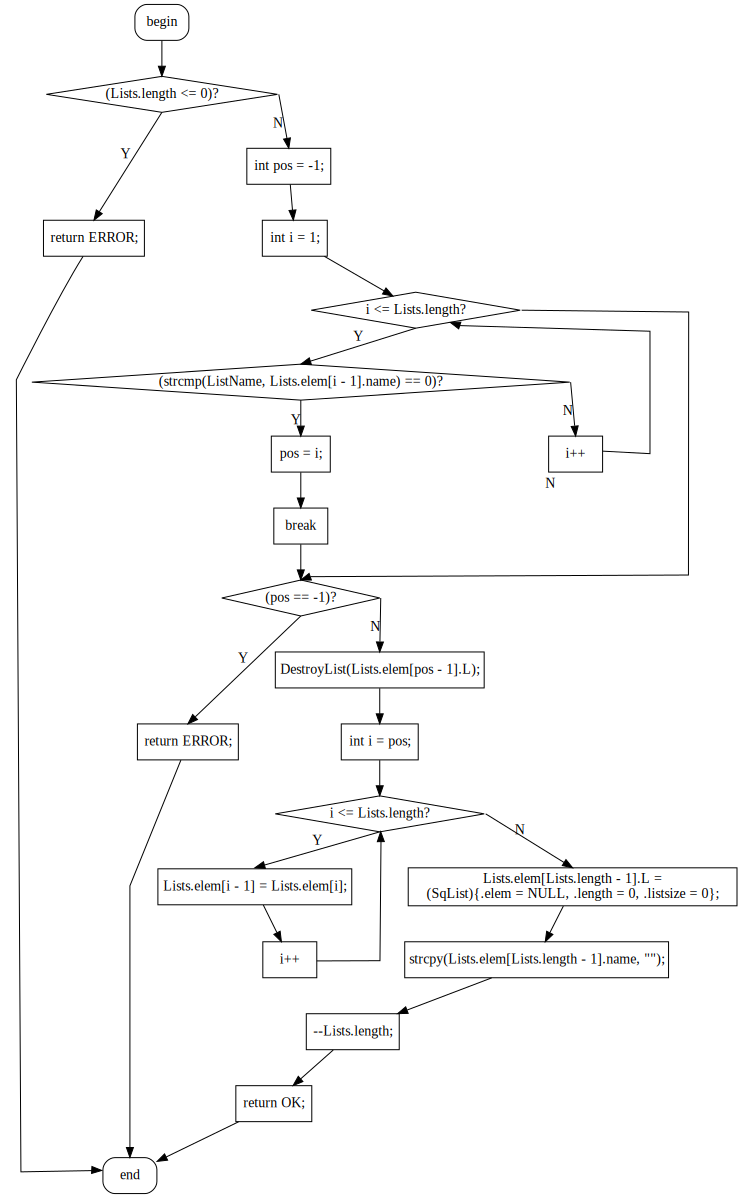
\includegraphics[width=4.0in]{flowchart/sq_list/flowchart/RemoveList.png}
	}
	\centering
	\caption{流程图}
	\label{fig6-6}
\end{figure}

\clearpage
\subsubsection{文件操作}

\subparagraph{SaveList}
\noindent
函数SaveList的签名如下:
\begin{lstlisting}[language=C++, frame=single]
status SaveList(SqList L, char FileName[]);
\end{lstlisting}

\noindent
实现: \\
先检查 L.elem,若为 NULL,则返回INFEASIBLE; \\
然后用 FileName 打开一个文件,如果发生错误,返回 ERROR; \\
接着依次用 fwrite 将 L.length 、L.listsize 、L.elem中元素写入文件; \\
最后关闭文件,返回 OK。\\

\subparagraph{LoadList}
\noindent
函数LoadList的签名如下:
\begin{lstlisting}[language=C++, frame=single]
status LoadList(SqList L, char FileName[]);
\end{lstlisting}

\noindent
实现: \\
先检查 L.elem,若为 NULL,则返回INFEASIBLE; \\
然后用 FileName 打开一个文件,如果发生错误,返回 ERROR; \\
接着声明变量 length、listsize,依次用 fread 将它们从文件读入; \\
然后声明一个 ElemType* 类型的指针 tmp,给它分配 listsize * sizeof(ElemType) 的内存,如果失败,返回ERROR; \\
申请内存成功后,把 length、listsize、tmp 依次赋值给 L.length、L.listsize、L.elem; \\
接着从文件读入 L.elem; \\
最后关闭文件,返回 OK。\\

\newpage

\subsubsection{算法}

\subparagraph{sort\_list}
\noindent
函数sort\_list的签名如下:
\begin{lstlisting}[language=C++, frame=single]
status sort_list(SqList &L);
\end{lstlisting}

\noindent
实现: \\
基于比较的排序算法时间复杂度下界为$O(nlogn)$。目前有多种排序算法能够达到此下界,包括但不限于快速排序、归并排序、堆排序等。gcc(libstdc++) 对std::sort的实现采用了一种叫introsort的算法,它优先采用快速排序,但在递归深度过深时切换到堆排序,同时在小区间上采用插入排序,较常规的随机化快速排序快数倍。\\
本实现采用常规的随机化快速排序。\\

\noindent
以下为生成随机数的函数:
\begin{lstlisting}[language=C++, frame=single]
#include <random>
int gen_rand(int l, int r) {
	std::random_device rand_device;

	std::default_random_engine e1(rand_device());
	std::uniform_int_distribution<int> uniform_dist(l, r);
	int mean = uniform_dist(e1);
	return mean;
}
\end{lstlisting}

\clearpage
\noindent
以下是partition函数的流程图。难点在于边界条件的判定。
\begin{figure}[H]
	\centering
	\subfloat{
		\centering
		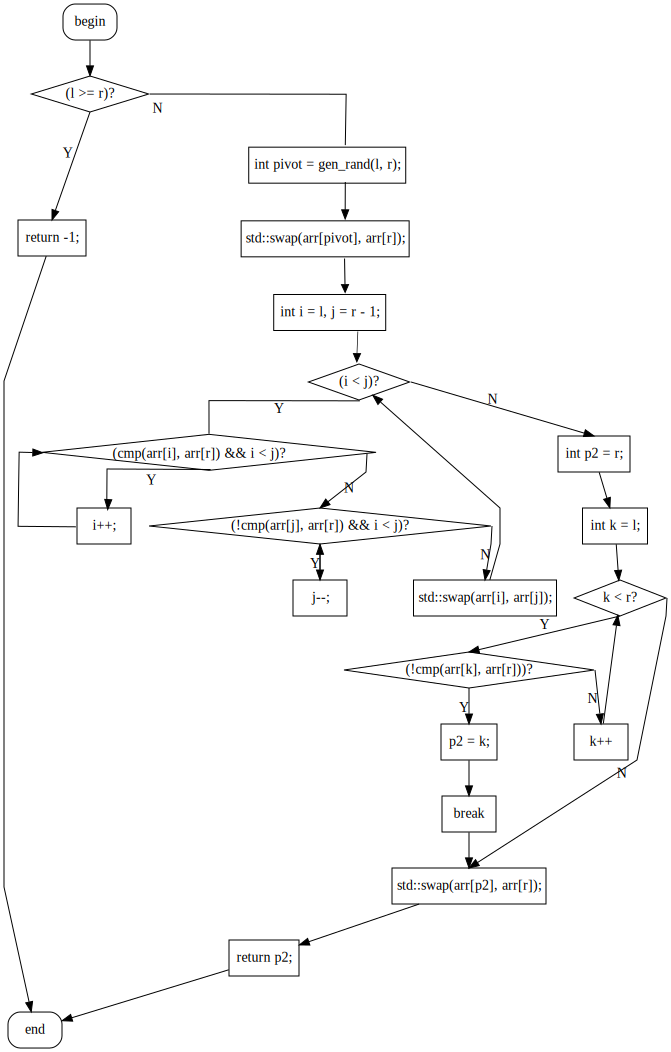
\includegraphics[width=4.0in]{flowchart/sq_list/flowchart/partition.png}
	}
	\centering
	\caption{流程图}
	\label{fig6-1}
\end{figure}


\newpage
\noindent
以下是快速排序函数的主体的流程图:
\begin{figure}[htbp]
	\centering
	\subfloat{
		\centering
		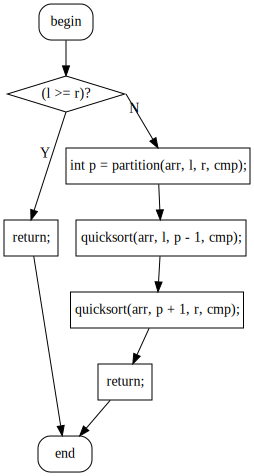
\includegraphics[width=3.0in]{flowchart/sq_list/flowchart/quicksort.png}
	}
	\centering
	\caption{流程图}
	\label{fig6-2}
\end{figure}

\subparagraph{max\_partial\_sum}
\noindent
函数max\_partial\_sum的签名如下:
\begin{lstlisting}[language=C++, frame=single]
ElemType max_partial_sum(SqList L);
\end{lstlisting}

\noindent
实现: \\
使用动态规划,以数组sum[i]表示以i为结尾的最大子数组和,则有如下递推式: $$sum[i] = max(sum[i - 1] + nums[i], nums[i])$$
求出sum[i]后,再找出最大的sum[i]即可。时间复杂度为$O(n)$.\\
\clearpage
流程图:
\begin{figure}[htbp]
	\centering
	\subfloat{
		\centering
		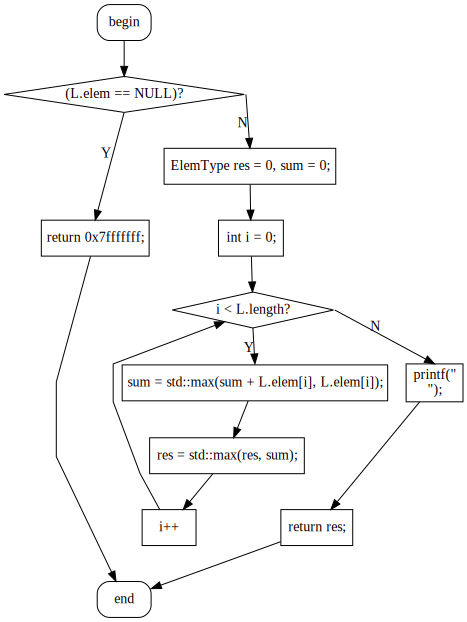
\includegraphics[width=3.0in]{flowchart/sq_list/flowchart/max_partial_sum.png}
	}
	\centering
	\caption{初始}
	\label{fig6-3}
\end{figure}

\subparagraph{k\_subarray}
\noindent
函数k\_subarray为和为k的子数组数目,签名如下:
\begin{lstlisting}[language=C++, frame=single]
int k_subarray(SqList &L, ElemType k);
\end{lstlisting}

\noindent
实现: \\
首先,考虑数组的前缀和sum[i]。和为k的连续数组满足: $$sum[i] - sum[j - 1] == k$$
即: $$sum[i] - k == sum[j - 1]$$
故只需考虑对于sum[i],有多少个满足该条件的sum[j - 1]。\\
为了能够快速找到sum[j - 1],我们可以使用哈希表存储这个信息.具体而言,我们声明一个哈希表sum\_map,以sum[j - 1]为键,sum[j - 1]出现的次数为值,从左到右更新sum\_map并计算答案。显然,每一次迭代中,sum[j - 1]对应的出现次数能够在$O(1)$内找到。同时,由于是从左往右更新答案,且sum[i]的计算只与前一项有关,故sum[i]可简化成current\_sum,表示该次迭代中的前缀和。\\
\clearpage
\noindent
流程图:
\begin{figure}[htbp]
	\centering
	\subfloat{
		\centering
		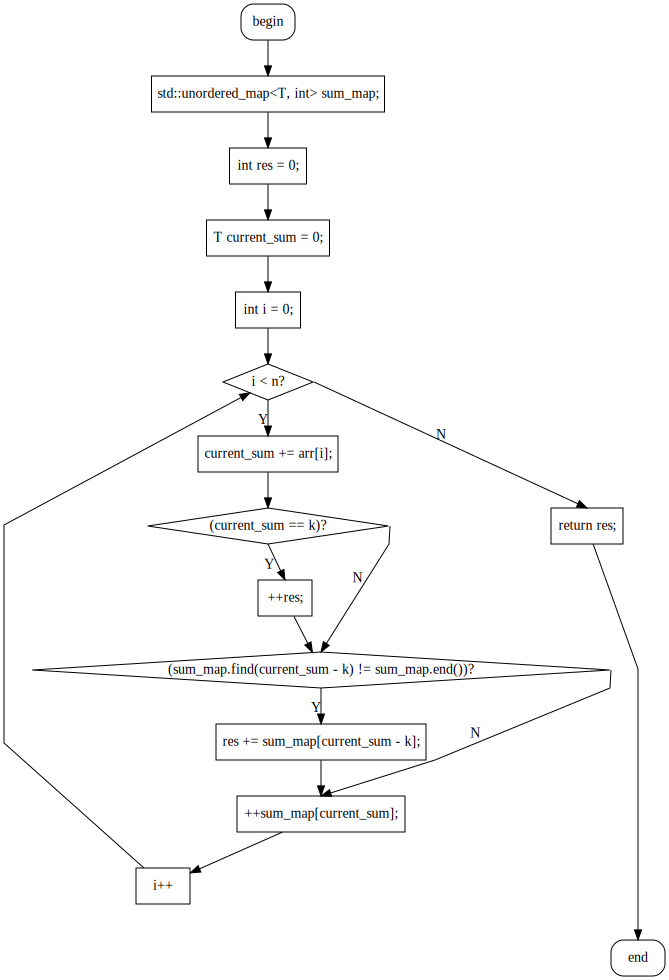
\includegraphics[width=3.5in]{flowchart/sq_list/flowchart/k_subarray.png}
	}
	\centering
	\caption{流程图}
	\label{fig6-4}
\end{figure}

\newpage

\subsection{系统测试}

\noindent
初始界面如下:
\begin{figure}[htbp]
	\centering
	\includegraphics[width=2.5in]{sq_list/initial_interface.png}
	\caption{初始界面}
	\label{fig1-1}
\end{figure}

\subsubsection{线性表操作}

\subparagraph{InitList}
\noindent
在初始界面中输入1,执行InitList操作,成功时如图所示
\begin{figure}[htbp]
	\centering
	\subfloat{
		\centering
		\includegraphics[width=2.3in]{sq_list/basic/InitList/InitList.png}
	}
	\centering
	\subfloat{
		\centering
		\includegraphics[width=2.3in]{sq_list/basic/InitList/InitList_after.png}
	} 
	\centering
	\caption{InitList成功}
	\label{fig1-2}
\end{figure}

\noindent
如果线性表已初始化,则提示:
\begin{figure}[htbp]
	\centering
	\subfloat{
		\centering
		\includegraphics[width=2.3in]{sq_list/basic/InitList/InitList_infeasible.png}
	}
	\centering
	\caption{InitList失败}
	\label{fig1-2}
\end{figure}

\subparagraph{DestroyList}
\noindent
在初始界面输入2,执行DestroyList操作,成功时如图所示:
\begin{figure}[htbp]
	\centering
	\subfloat{
		\centering
		\includegraphics[width=2.3in]{sq_list/basic/DestroyList/DestroyList.png}
	}
	\centering
	\subfloat{
		\centering
		\includegraphics[width=2.3in]{sq_list/basic/DestroyList/DestroyList_after.png}
	} 
	\centering
	\caption{DestroyList成功}
	\label{fig1-3}
\end{figure}

\noindent
如果线性表未初始化,则提示:
\begin{figure}[htbp]
	\centering
	\subfloat{
		\centering
		\includegraphics[width=2.3in]{sq_list/basic/DestroyList/DestroyList_infeasible.png}
	}
	\centering
	\caption{InitList失败}
	\label{fig1-4}
\end{figure}

\subparagraph{ListEmpty}
\noindent
首先创建一个空表:
\begin{figure}[htbp]
	\centering
	\subfloat{
		\centering
		\includegraphics[width=2.3in]{sq_list/basic/ListEmpty/prelude1.png}
	}
	\centering
	\subfloat{
		\centering
		\includegraphics[width=2.3in]{sq_list/basic/ListEmpty/prelude2.png}
	} 
	\centering
	\caption{创建空表}
	\label{fig1-5}
\end{figure}

\clearpage
\noindent
然后在初始界面输入4。输出如下:
\begin{figure}[htbp]
	\centering
	\subfloat{
		\centering
		\includegraphics[width=2.3in]{sq_list/basic/ListEmpty/ok.png}
	}
	\centering
	\caption{线性表是空表}
	\label{fig1-6}
\end{figure}

\noindent
接着插入一些元素(用到了自己增加的"批量插入"功能):
\begin{figure}[htbp]
	\centering
	\subfloat{
		\centering
		\includegraphics[width=2.3in]{sq_list/basic/ListEmpty/prelude3.png}
	}
	\centering
	\caption{插入元素}
	\label{fig1-7}
\end{figure}

\noindent
然后执行功能4:
\begin{figure}[htbp]
	\centering
	\subfloat{
		\centering
		\includegraphics[width=2.3in]{sq_list/basic/ListEmpty/error.png}
	}
	\centering
	\caption{线性表不是空表}
	\label{fig1-8}
\end{figure}

\clearpage
\noindent
对于线性表未初始化的情况:
\begin{figure}[htbp]
	\centering
	\subfloat{
		\centering
		\includegraphics[width=2.3in]{sq_list/basic/ListEmpty/infeasible.png}
	}
	\centering
	\caption{插入元素}
	\label{fig1-9}
\end{figure}

\subparagraph{ClearList}
\noindent
首先创建一个空表,并插入元素:
\begin{figure}[htbp]
	\centering
	\subfloat{
		\centering
		\includegraphics[width=2.1in]{sq_list/basic/ClearList/prelude1.png}
	}
	\centering
	\subfloat{
		\centering
		\includegraphics[width=2.1in]{sq_list/basic/ClearList/prelude2.png}
	} 
	\centering
	\caption{初始}
	\label{fig1-10}
\end{figure}

\noindent
然后在初始界面输入3,执行ClearList操作,成功时如图所示:
\begin{figure}[htbp]
	\centering
	\subfloat{
		\centering
		\includegraphics[width=2.1in]{sq_list/basic/ClearList/clear_list.png}
	}
	\centering
	\subfloat{
		\centering
		\includegraphics[width=2.1in]{sq_list/basic/ClearList/clear_list_after.png}
	} 
	\centering
	\caption{ClearList成功}
	\label{fig1-11}
\end{figure}

\clearpage
\noindent
现在执行InitList操作,失败,符合ClearList的语义.
\begin{figure}[htbp]
	\centering
	\subfloat{
		\centering
		\includegraphics[width=2.3in]{sq_list/basic/ClearList/init_after_clear.png}
	}
	\centering
	\caption{ClearList失败}
	\label{fig1-12}
\end{figure}

\noindent
现在表是空表。再执行一遍功能3:
\begin{figure}[htbp]
	\centering
	\subfloat{
		\centering
		\includegraphics[width=2.3in]{sq_list/basic/ClearList/error.png}
	}
	\centering
	\caption{ClearList失败}
	\label{fig1-13}
\end{figure}

\noindent
对未初始化的线性表进行操作:
\begin{figure}[htbp]
	\centering
	\subfloat{
		\centering
		\includegraphics[width=2.3in]{sq_list/basic/ClearList/infeasible.png}
	}
	\centering
	\caption{INFEASIBLE}
	\label{fig1-14}
\end{figure}

\clearpage
\subparagraph{ListLength}
\noindent
首先创建一个空表:
\begin{figure}[htbp]
	\centering
	\subfloat{
		\centering
		\includegraphics[width=2.1in]{sq_list/basic/ListLength/prelude1.png}
	}
	\centering
	\caption{初始}
	\label{fig1-15}
\end{figure}

\noindent
然后执行操作5。现在表是空表.
\begin{figure}[htbp]
	\centering
	\subfloat{
		\centering
		\includegraphics[width=2.1in]{sq_list/basic/ListLength/empty_list.png}
	}
	\centering
	\caption{空表}
	\label{fig1-16}
\end{figure}

\noindent
接着添加元素:
\begin{figure}[htbp]
	\centering
	\subfloat{
		\centering
		\includegraphics[width=2.1in]{sq_list/basic/ListLength/prelude2.png}
	}
	\centering
	\caption{添加元素}
	\label{fig1-17}
\end{figure}

\clearpage
\noindent
再进行一遍操作5。可以看到,表长变成了7.
\begin{figure}[htbp]
	\centering
	\subfloat{
		\centering
		\includegraphics[width=2.1in]{sq_list/basic/ListLength/normal_list.png}
	}
	\centering
	\caption{非空的表}
	\label{fig1-18}
\end{figure}

\noindent
对未初始化的表:
\begin{figure}[htbp]
	\centering
	\subfloat{
		\centering
		\includegraphics[width=2.1in]{sq_list/basic/ListLength/infeasible.png}
	}
	\centering
	\caption{INFEASIBLE}
	\label{fig1-19}
\end{figure}

\subparagraph{ListTraverse}
\noindent
首先创建空表并添加元素:
\begin{figure}[htbp]
	\centering
	\subfloat{
		\centering
		\includegraphics[width=2.1in]{sq_list/basic/ListTraverse/prelude1.png}
	}
	\centering
	\subfloat{
		\centering
		\includegraphics[width=2.1in]{sq_list/basic/ListTraverse/prelude2.png}
	}
	\centering
	\caption{初始}
	\label{fig1-20}
\end{figure}

\clearpage
\noindent
然后执行操作12:
\begin{figure}[htbp]
	\centering
	\subfloat{
		\centering
		\includegraphics[width=2.1in]{sq_list/basic/ListTraverse/ok.png}
	}
	\centering
	\caption{ListTraverse成功}
	\label{fig1-21}
\end{figure}

\subparagraph{GetElem}
\noindent
首先创建空表并添加元素:
\begin{figure}[htbp]
	\centering
	\subfloat{
		\centering
		\includegraphics[width=2.1in]{sq_list/basic/GetElem/prelude1.png}
	}
	\centering
	\subfloat{
		\centering
		\includegraphics[width=2.1in]{sq_list/basic/GetElem/prelude2.png}
	}
	\centering
	\caption{初始}
	\label{fig1-22}
\end{figure}

\noindent
然后执行操作6。可以看到,操作界面输出了对应位置的元素值.
\begin{figure}[htbp]
	\centering
	\subfloat{
		\centering
		\includegraphics[width=2.1in]{sq_list/basic/GetElem/ok.png}
	}
	\centering
	\caption{GetElem成功}
	\label{fig1-23}
\end{figure}

\clearpage
\noindent
下面输入一个越界的数据,操作界面提示了一个错误.
\begin{figure}[htbp]
	\centering
	\subfloat{
		\centering
		\includegraphics[width=2.1in]{sq_list/basic/GetElem/error.png}
	}
	\centering
	\caption{GetElem失败}
	\label{fig1-24}
\end{figure}

\noindent
对未初始化的线性表进行操作:
\begin{figure}[htbp]
	\centering
	\subfloat{
		\centering
		\includegraphics[width=2.1in]{sq_list/basic/GetElem/infeasible.png}
	}
	\centering
	\caption{INFEASIBLE}
	\label{fig1-25}
\end{figure}

\clearpage
\subparagraph{LocateElem}
\noindent
首先创建空表并添加元素:
\begin{figure}[htbp]
	\centering
	\subfloat{
		\centering
		\includegraphics[width=2.2in]{sq_list/basic/LocateElem/prelude1.png}
	}
	\centering
	\subfloat{
		\centering
		\includegraphics[width=2.2in]{sq_list/basic/LocateElem/prelude2.png}
	}
	\centering
	\caption{初始}
	\label{fig1-26}
\end{figure}

\noindent
下面输入一个只出现过一次的数据,操作界面输出它的位置.
\begin{figure}[htbp]
	\centering
	\subfloat{
		\centering
		\includegraphics[width=2.1in]{sq_list/basic/LocateElem/ok_unique.png}
	}
	\centering
	\caption{LocateElem成功\_1}
	\label{fig1-27}
\end{figure}

\noindent
下面输入一个重复出现的数据,操作界面输出它第一次出现的位置.
\begin{figure}[htbp]
	\centering
	\subfloat{
		\centering
		\includegraphics[width=2.1in]{sq_list/basic/LocateElem/ok_repeated.png}
	}
	\centering
	\caption{LocateElem成功\_2}
	\label{fig1-28}
\end{figure}

\clearpage
\noindent
下面输入一个表中没有的数据,操作界面提示错误.
\begin{figure}[htbp]
	\centering
	\subfloat{
		\centering
		\includegraphics[width=2.1in]{sq_list/basic/LocateElem/error.png}
	}
	\centering
	\caption{LocateElem失败}
	\label{fig1-29}
\end{figure}

\noindent
线性表未初始化时:
\begin{figure}[htbp]
	\centering
	\subfloat{
		\centering
		\includegraphics[width=2.1in]{sq_list/basic/LocateElem/infeasible.png}
	}
	\centering
	\caption{INFEASIBLE}
	\label{fig1-30}
\end{figure}

\subparagraph{PriorElem}
\noindent
首先创建空表并添加元素:
\begin{figure}[htbp]
	\centering
	\subfloat{
		\centering
		\includegraphics[width=2.2in]{sq_list/basic/PriorElem/prelude1.png}
	}
	\centering
	\subfloat{
		\centering
		\includegraphics[width=2.2in]{sq_list/basic/PriorElem/prelude2.png}
	}
	\centering
	\caption{初始}
	\label{fig1-31}
\end{figure}

\clearpage
\noindent
下面输入一个只出现过一次的数据,操作界面输出它的前驱.
\begin{figure}[htbp]
	\centering
	\subfloat{
		\centering
		\includegraphics[width=2.2in]{sq_list/basic/PriorElem/ok_unique.png}
	}
	\centering
	\caption{PriorElem成功\_1}
	\label{fig1-32}
\end{figure}

\noindent
下面输入一个重复出现的数据,操作界面输出它第一次出现位置的前驱元素.
\begin{figure}[htbp]
	\centering
	\subfloat{
		\centering
		\includegraphics[width=2.1in]{sq_list/basic/PriorElem/ok_repeated.png}
	}
	\centering
	\caption{PriorElem成功\_2}
	\label{fig1-33}
\end{figure}

\noindent
下面输入一个没有前驱的数据,操作界面提示错误.
\begin{figure}[htbp]
	\centering
	\subfloat{
		\centering
		\includegraphics[width=2.1in]{sq_list/basic/PriorElem/error.png}
	}
	\centering
	\caption{PriorElem失败}
	\label{fig1-34}
\end{figure}

\clearpage
\noindent
线性表未初始化时:
\begin{figure}[htbp]
	\centering
	\subfloat{
		\centering
		\includegraphics[width=2.1in]{sq_list/basic/PriorElem/infeasible.png}
	}
	\centering
	\caption{INFEASIBLE}
	\label{fig1-35}
\end{figure}

\subparagraph{NextElem}
\noindent
首先创建空表并添加元素:
\begin{figure}[htbp]
	\centering
	\subfloat{
		\centering
		\includegraphics[width=2.2in]{sq_list/basic/NextElem/prelude1.png}
	}
	\centering
	\subfloat{
		\centering
		\includegraphics[width=2.2in]{sq_list/basic/NextElem/prelude2.png}
	}
	\centering
	\caption{初始}
	\label{fig1-36}
\end{figure}

\noindent
下面输入一个只出现过一次的数据,操作界面输出它的后继.
\begin{figure}[htbp]
	\centering
	\subfloat{
		\centering
		\includegraphics[width=2.2in]{sq_list/basic/NextElem/ok_unique.png}
	}
	\centering
	\caption{NextElem成功\_1}
	\label{fig1-37}
\end{figure}

\clearpage
\noindent
下面输入一个重复出现的数据,操作界面输出它第一次出现位置的后继元素.
\begin{figure}[htbp]
	\centering
	\subfloat{
		\centering
		\includegraphics[width=2.1in]{sq_list/basic/NextElem/ok_repeated.png}
	}
	\centering
	\caption{NextElem成功\_2}
	\label{fig1-38}
\end{figure}

\noindent
下面输入一个没有后继的数据,操作界面提示错误.
\begin{figure}[htbp]
	\centering
	\subfloat{
		\centering
		\includegraphics[width=2.1in]{sq_list/basic/NextElem/error.png}
	}
	\centering
	\caption{NextElem失败}
	\label{fig1-39}
\end{figure}

\noindent
线性表未初始化时:
\begin{figure}[htbp]
	\centering
	\subfloat{
		\centering
		\includegraphics[width=2.1in]{sq_list/basic/NextElem/infeasible.png}
	}
	\centering
	\caption{INFEASIBLE}
	\label{fig1-40}
\end{figure}

\clearpage
\subparagraph{ListInsert}
\noindent
首先创建空表并添加元素:
\begin{figure}[htbp]
	\centering
	\subfloat{
		\centering
		\includegraphics[width=2.2in]{sq_list/basic/ListInsert/prelude1.png}
	}
	\centering
	\subfloat{
		\centering
		\includegraphics[width=2.2in]{sq_list/basic/ListInsert/prelude2.png}
	}
	\centering
	\caption{初始}
	\label{fig1-41}
\end{figure}

\noindent
下面将一个元素插入到线性表的中间位置,再进行遍历。可以看到,遍历的结果是正确的.
\begin{figure}[htbp]
	\centering
	\subfloat{
		\centering
		\includegraphics[width=2.2in]{sq_list/basic/ListInsert/ok1_1.png}
	}
	\subfloat{
		\centering
		\includegraphics[width=2.2in]{sq_list/basic/ListInsert/ok1_2.png}
	}
	\centering
	\caption{ListInsert成功\_1}
	\label{fig1-42}
\end{figure}

\noindent
然后将一个元素插入到线性表的末尾,再进行遍历。可以看到,遍历的结果是正确的.
\begin{figure}[htbp]
	\centering
	\subfloat{
		\centering
		\includegraphics[width=2.2in]{sq_list/basic/ListInsert/ok2_1.png}
	}
	\subfloat{
		\centering
		\includegraphics[width=2.2in]{sq_list/basic/ListInsert/ok2_2.png}
	}
	\centering
	\caption{ListInsert成功\_2}
	\label{fig1-43}
\end{figure}

\clearpage
\noindent
下面将元素插入到错误的位置(分别是表的末尾以后和开头之前),均产生错误.
\begin{figure}[htbp]
	\centering
	\subfloat{
		\centering
		\includegraphics[width=2.3in]{sq_list/basic/ListInsert/error1.png}
	}
	\subfloat{
		\centering
		\includegraphics[width=2.1in]{sq_list/basic/ListInsert/error2.png}
	}
	\centering
	\caption{ListInsert失败}
	\label{fig1-44}
\end{figure}

\noindent
线性表未初始化时:
\begin{figure}[htbp]
	\centering
	\subfloat{
		\centering
		\includegraphics[width=2.1in]{sq_list/basic/ListInsert/infeasible.png}
	}
	\centering
	\caption{INFEASIBLE}
	\label{fig1-45}
\end{figure}

\subparagraph{ListDelete}
\noindent
为方便起见,使用ListInsert操作后的数据来测试.\\
下面删除一个线性表中间位置的元素,再进行遍历。可以看到,遍历的结果是正确的.
\begin{figure}[htbp]
	\centering
	\subfloat{
		\centering
		\includegraphics[width=2.2in]{sq_list/basic/ListDelete/ok1_1.png}
	}
	\subfloat{
		\centering
		\includegraphics[width=2.2in]{sq_list/basic/ListDelete/ok1_2.png}
	}
	\centering
	\caption{ListDelete成功\_1}
	\label{fig1-46}
\end{figure}

\clearpage
\noindent
然后删除线性表末尾的元素,再进行遍历。可以看到,遍历的结果是正确的.
\begin{figure}[htbp]
	\centering
	\subfloat{
		\centering
		\includegraphics[width=2.2in]{sq_list/basic/ListDelete/ok2_1.png}
	}
	\subfloat{
		\centering
		\includegraphics[width=2.2in]{sq_list/basic/ListDelete/ok2_2.png}
	}
	\centering
	\caption{ListDelete成功\_2}
	\label{fig1-47}
\end{figure}

\noindent
下面删除错误位置的元素(分别是表的末尾以后和开头之前),均产生错误.
\begin{figure}[htbp]
	\centering
	\subfloat{
		\centering
		\includegraphics[width=2.3in]{sq_list/basic/ListDelete/error1.png}
	}
	\subfloat{
		\centering
		\includegraphics[width=2.1in]{sq_list/basic/ListDelete/error2.png}
	}
	\centering
	\caption{ListDelete失败}
	\label{fig1-48}
\end{figure}

\noindent
线性表未初始化时:
\begin{figure}[htbp]
	\centering
	\subfloat{
		\centering
		\includegraphics[width=2.1in]{sq_list/basic/ListDelete/infeasible.png}
	}
	\centering
	\caption{INFEASIBLE}
	\label{fig1-49}
\end{figure}

\newpage

\subsubsection{多线性表管理}
操作界面如下:
\begin{figure}[htbp]
	\centering
	\subfloat{
		\centering
		\includegraphics[width=2.1in]{sq_list/multi_list/interface.png}
	}
	\centering
	\caption{操作界面}
	\label{fig2-1}
\end{figure}

\subparagraph{AddList}
\noindent
首先进行操作1,输入待添加线性表的名字ok\_computer,操作界面显示插入成功.
\begin{figure}[htbp]
	\centering
	\subfloat{
		\centering
		\includegraphics[width=2.1in]{sq_list/multi_list/AddList/ok1_1.png}
	}
	\centering
	\caption{AddList成功}
	\label{fig2-2}
\end{figure}

\noindent
回到操作界面后,我们发现线性表多了一个ok\_computer.
\begin{figure}[htbp]
	\centering
	\subfloat{
		\centering
		\includegraphics[width=2.1in]{sq_list/multi_list/AddList/ok1_2.png}
	}
	\centering
	\caption{AddList成功}
	\label{fig2-3}
\end{figure}

\clearpage
\subparagraph{切换线性表}
\noindent
这个功能没有做成函数,姑且看一下吧.\\
先看一下错误情况,即没有这个线性表:
\begin{figure}[htbp]
	\centering
	\subfloat{
		\centering
		\includegraphics[width=2.1in]{sq_list/multi_list/SwitchList/error.png}
	}
	\centering
	\caption{切换失败}
	\label{fig2-4}
\end{figure}

\noindent
如果有这个线性表,那么切换成功。回到操作界面以后,星号在切换到的表上.
\begin{figure}[htbp]
	\centering
	\subfloat{
		\centering
		\includegraphics[width=2.1in]{sq_list/multi_list/SwitchList/ok1_1.png}
	}
	\subfloat{
		\centering
		\includegraphics[width=2.1in]{sq_list/multi_list/SwitchList/ok1_2.png}
	}
	\centering
	\caption{切换成功\_1}
	\label{fig2-5}
\end{figure}

\noindent
现在回到主界面,查看我们刚刚建的新表。很显然,它是个空表.
\begin{figure}[htbp]
	\centering
	\subfloat{
		\centering
		\includegraphics[width=2.1in]{sq_list/multi_list/SwitchList/ok1_3.png}
	}
	\subfloat{
		\centering
		\includegraphics[width=2.1in]{sq_list/multi_list/SwitchList/ok1_4.png}
	}
	\centering
	\caption{切换成功\_2}
	\label{fig2-6}
\end{figure}

\clearpage
\noindent
现在对新表插入元素,再切换到旧表。遍历一遍旧表,发现对新表的操作并不影响旧表的数据.
\begin{figure}[htbp]
	\centering
	\subfloat{
		\centering
		\includegraphics[width=2.0in]{sq_list/multi_list/SwitchList/ok1_5.png}
	}
	\centering
	\subfloat{
		\centering
		\includegraphics[width=2.0in]{sq_list/multi_list/SwitchList/ok1_6.png}
	}
	\centering
	\subfloat{
		\centering
		\includegraphics[width=2.0in]{sq_list/multi_list/SwitchList/ok1_7.png}
	}
	\centering
	\caption{切换成功\_3}
	\label{fig2-7}
\end{figure}

\subparagraph{LocateList}
\noindent
先看一下错误情况,即没有这个线性表:
\begin{figure}[htbp]
	\centering
	\subfloat{
		\centering
		\includegraphics[width=2.5in]{sq_list/multi_list/LocateList/error.png}
	}
	\centering
	\caption{查找失败}
	\label{fig2-8}
\end{figure}

\noindent
再看一下正确情况,即有这个线性表:
\begin{figure}[htbp]
	\centering
	\subfloat{
		\centering
		\includegraphics[width=2.5in]{sq_list/multi_list/LocateList/ok_1.png}
	}
	\centering
	\caption{查找成功}
	\label{fig2-9}
\end{figure}

\clearpage
\subparagraph{RemoveList}
\noindent
先看一下错误情况,即没有这个线性表:
\begin{figure}[htbp]
	\centering
	\subfloat{
		\centering
		\includegraphics[width=2.5in]{sq_list/multi_list/RemoveList/error.png}
	}
	\centering
	\caption{删除失败}
	\label{fig2-10}
\end{figure}

\noindent
如果有这个线性表,那么删除成功。\\
如果被删除的线性表就是现在正进行操作的线性表,则删除后线性表指针切换到头一个线性表.查找、切换到原来的线性表,均显示未找到.
\begin{figure}[htbp]
	\centering
	\subfloat{
		\centering
		\includegraphics[width=2.1in]{sq_list/multi_list/RemoveList/ok1_1.png}
	}
	\subfloat{
		\centering
		\includegraphics[width=2.1in]{sq_list/multi_list/RemoveList/ok1_2.png}
	}
	\subfloat{
		\centering
		\includegraphics[width=2.1in]{sq_list/multi_list/RemoveList/ok1_3.png}
	}
	\centering
	\caption{删除成功\_1}
	\label{fig2-11}
\end{figure}

\noindent
看一下现在的线性表。可以看到数据不受影响.
\begin{figure}[htbp]
	\centering
	\subfloat{
		\centering
		\includegraphics[width=2.1in]{sq_list/multi_list/RemoveList/ok1_4.png}
	}
	\centering
	\caption{删除成功\_2}
	\label{fig2-12}
\end{figure}

\clearpage
\noindent
如果被删除的线性表不是现在正进行操作的线性表,则删除后线性表指针不变.
\begin{figure}[htbp]
	\centering
	\subfloat{
		\centering
		\includegraphics[width=2.1in]{sq_list/multi_list/RemoveList/ok2_1.png}
	}
	\subfloat{
		\centering
		\includegraphics[width=2.1in]{sq_list/multi_list/RemoveList/ok2_2.png}
	}
	\subfloat{
		\centering
		\includegraphics[width=2.1in]{sq_list/multi_list/RemoveList/ok2_3.png}
	}
	\centering
	\caption{删除成功\_3}
	\label{fig2-13}
\end{figure}

\noindent
如果只剩一个线性表,让我们删掉它:
\begin{figure}[htbp]
	\centering
	\subfloat{
		\centering
		\includegraphics[width=2.1in]{sq_list/multi_list/RemoveList/ok3_1.png}
	}
	\centering
	\caption{删除成功\_4}
	\label{fig2-14}
\end{figure}

\noindent
删除后,各种操作均失效,需要添加线性表:
\begin{figure}[htbp]
	\centering
	\subfloat{
		\centering
		\includegraphics[width=2.1in]{sq_list/multi_list/RemoveList/ok3_2.png}
	}
	\subfloat{
		\centering
		\includegraphics[width=2.1in]{sq_list/multi_list/RemoveList/ok3_3.png}
	}
	\subfloat{
		\centering
		\includegraphics[width=2.1in]{sq_list/multi_list/RemoveList/ok3_4.png}
	}
	\centering
	\caption{删除成功\_5}
	\label{fig2-15}
\end{figure}

\newpage
\subsubsection{文件操作}
\noindent
文件操作的操作界面:
\begin{figure}[htbp]
	\centering
	\subfloat{
		\centering
		\includegraphics[width=2.5in]{sq_list/file_io/interface.png}
	}
	\centering
	\caption{文件操作\_1}
	\label{fig3-1}
\end{figure}

\noindent
首先新建一个线性表,并插入元素:
\begin{figure}[htbp]
	\centering
	\subfloat{
		\centering
		\includegraphics[width=2.1in]{sq_list/file_io/prelude.png}
	}
	\centering
	\caption{初始}
	\label{fig3-2}
\end{figure}

\noindent
然后把它保存到../list3.dat(程序运行在build目录):
\begin{figure}[htbp]
	\centering
	\subfloat{
		\centering
		\includegraphics[width=2.1in]{sq_list/file_io/save_ok_1.png}
	}
	\centering
	\caption{保存成功\_1}
	\label{fig3-3}
\end{figure}

\clearpage
\noindent
现在看一看目录树,发现根目录下有一个新增的list3.dat:
\begin{figure}[htbp]
	\centering
	\subfloat{
		\centering
		\includegraphics[width=2.1in]{sq_list/file_io/save_ok_2.png}
	}
	\centering
	\caption{保存成功\_2}
	\label{fig3-4}
\end{figure}

\noindent
现在添加一个新表:
\begin{figure}[htbp]
	\centering
	\subfloat{
		\centering
		\includegraphics[width=2.1in]{sq_list/file_io/load_prelude_1.png}
	}
	\centering
	\caption{加载\_初始}
	\label{fig3-5}
\end{figure}


\noindent
在文件的操作界面中选择1,输入加载的文件名,如果文件不存在,就会提示错误:
\begin{figure}[htbp]
	\centering
	\subfloat{
		\centering
		\includegraphics[width=2.1in]{sq_list/file_io/load_error.png}
	}
	\centering
	\caption{加载成功\_1}
	\label{fig3-6}
\end{figure}

\clearpage
\noindent
文件存在时,提示加载成功:
\begin{figure}[htbp]
	\centering
	\subfloat{
		\centering
		\includegraphics[width=2.1in]{sq_list/file_io/load_ok_1.png}
	}
	\centering
	\caption{加载成功\_1}
	\label{fig3-7}
\end{figure}

\noindent
回到主界面,遍历线性表,可以看到文件当中的数据已经加载进了表里:
\begin{figure}[htbp]
	\centering
	\subfloat{
		\centering
		\includegraphics[width=2.1in]{sq_list/file_io/load_ok_2.png}
	}
	\centering
	\caption{加载成功\_2}
	\label{fig3-8}
\end{figure}

\noindent
现在,我们要从另一个文件中加载数据,并且覆盖掉这张已经有数据的表。先看看它原来的样子:
\begin{figure}[htbp]
	\centering
	\subfloat{
		\centering
		\includegraphics[width=2.1in]{sq_list/file_io/load_and_cover_ok_1.png}
	}
	\centering
	\caption{加载并覆盖成功\_初始}
	\label{fig3-9}
\end{figure}

\clearpage
\noindent
切换到文件的操作界面,输入一个不存在的文件名,提示出错:
\begin{figure}[htbp]
	\centering
	\subfloat{
		\centering
		\includegraphics[width=2.5in]{sq_list/file_io/load_and_cover_error.png}
	}
	\centering
	\caption{加载并覆盖失败}
	\label{fig3-10}
\end{figure}

\noindent
输入一个存在的文件名,则提示成功并输出覆盖后的表。(114514并不是乱码)
\begin{figure}[htbp]
	\centering
	\subfloat{
		\centering
		\includegraphics[width=2.5in]{sq_list/file_io/load_and_cover_ok_2.png}
	}
	\centering
	\caption{加载并覆盖成功\_1}
	\label{fig3-11}
\end{figure}

\noindent
这里给出list.dat的二进制编码:
\begin{figure}[htbp]
	\centering
	\subfloat{
		\centering
		\includegraphics[width=3.0in]{sq_list/file_io/list_dat.png}
	}
	\centering
	\caption{list.dat}
	\label{fig3-12}
\end{figure}

\noindent
切换到主界面,遍历一遍该表,可以发现数据也是如此:
\begin{figure}[H]
	\centering
	\subfloat{
		\centering
		\includegraphics[width=2.5in]{sq_list/file_io/load_and_cover_ok_3.png}
	}
	\centering
	\caption{加载并覆盖成功\_2}
	\label{fig3-13}
\end{figure}

\newpage

\subsubsection{算法}
\noindent
算法的操作界面如下:
\begin{figure}[htbp]
	\centering
	\subfloat{
		\centering
		\includegraphics[width=2.5in]{sq_list/algo/interface.png}
	}
	\centering
	\caption{加载并覆盖成功\_2}
	\label{fig4-1}
\end{figure}

\subparagraph{sort\_list}
\noindent
首先创建一个线性表并插入元素:
\begin{figure}[htbp]
	\centering
	\subfloat{
		\centering
		\includegraphics[width=2.5in]{sq_list/algo/sort_list/prelude.png}
	}
	\centering
	\caption{排序}
	\label{fig4-2}
\end{figure}

\noindent
然后切换到算法菜单,输入2对其进行排序,界面会输出排序过后的线性表:
\begin{figure}[htbp]
	\centering
	\subfloat{
		\centering
		\includegraphics[width=2.5in]{sq_list/algo/sort_list/result.png}
	}
	\centering
	\caption{排序结果}
	\label{fig4-3}
\end{figure}

\clearpage
\subparagraph{max\_partial\_sum}
\noindent
首先创建一个线性表并插入元素:
\begin{figure}[htbp]
	\centering
	\subfloat{
		\centering
		\includegraphics[width=2.5in]{sq_list/algo/max_partial_sum/prelude.png}
	}
	\centering
	\caption{最大子段和}
	\label{fig4-4}
\end{figure}

\noindent
然后切换到算法界面,输入1,界面输出最大子段和:
\begin{figure}[htbp]
	\centering
	\subfloat{
		\centering
		\includegraphics[width=2.5in]{sq_list/algo/max_partial_sum/result.png}
	}
	\centering
	\caption{排序}
	\label{fig4-5}
\end{figure}

\subparagraph{k\_subarray}
\noindent
首先创建一个线性表并插入元素:
\begin{figure}[htbp]
	\centering
	\subfloat{
		\centering
		\includegraphics[width=2.5in]{sq_list/algo/k_subarray/prelude.png}
	}
	\centering
	\caption{和为k的连续子数组\_初始}
	\label{fig4-6}
\end{figure}

\clearpage
\noindent
然后切换到算法界面,输入3进入该功能,然后输入k值,界面输出和为k的子数组数目:
\begin{figure}[htbp]
	\centering
	\subfloat{
		\centering
		\includegraphics[width=2.5in]{sq_list/algo/k_subarray/result1.png}
	}
	\centering
	\caption{和为k的连续子数组\_1}
	\label{fig4-7}
\end{figure}

\noindent
换一个k值:
\begin{figure}[htbp]
	\centering
	\subfloat{
		\centering
		\includegraphics[width=2.5in]{sq_list/algo/k_subarray/result2.png}
	}
	\centering
	\caption{和为k的连续子数组\_2}
	\label{fig4-8}
\end{figure}

\newpage
\subsubsection{一些小功能}
\noindent
主程序里的示例代码里有一句:
\begin{lstlisting}[language=C++, frame=single]
system("cls");
\end{lstlisting}
这对*nix系统来说并不友好,因此需要封装一个多平台版本:
\begin{lstlisting}[language=C++, frame=single]
void clean_terminal() {
#if defined(__APPLE__) || defined(__linux__) || defined(__FreeBSD__)
	system("export TERM=xterm && reset");  // *nix
#elif defined(_WIN32)
	system("cls");  // windows
#endif
	return;
}
\end{lstlisting}

\newpage

\subsection{实验小结}

该实验难度不大,但是附加功能和代码整合有一定难度.

先说说代码整合。由于本项目代码量较大,如果每一个小功能都新建一个文件,那将会很丑陋,也会给代码构建造成很大困扰。因此,有必要把同类型的功能归于一个文件中。同时,对于C/C++,函数的声明与实现分离,也是正式项目中惯常的做法。一般把结构体定义与函数声明放到.h文件,而函数实现放到.c/.cpp文件中。头文件和实现分别放在src和include目录下(似乎是因为链接第三方库的需要,不过线性表这个项目其实用不到).这里有个坑: 如果用了C++的模板,这么做会出现链接问题。解决方法是把模板函数放到.hpp文件中,再如同\#include "xxx.h"文件一样include它.

然后是附加功能,尤其是文件操作和多线性表管理.

首先是文件操作。据观察,诸多学生被误用fscanf/fprintf产生的预料之外的错误消耗掉了大量时间。线性表的数据格式较为简单,因而难度还算可以接受; 数据格式的复杂性将会在后面的实验中大大凸显.

然后是多线性表管理。指向当前多线性表的指针被声明在线性表管理表的结构体之外,徒增许多难度。一方面,它使得切换线性表的操作与其他操作形式上不统一; 另一方面,删除操作的函数内部无法很好地利用这个指针。这一问题曾造成了删除后指针指向不正确的bug。另外,删除线性表的操作较为复杂。它涉及查找、销毁、移动等操作,稍有不慎就会遗漏其中某个方面。幸运的是,C语言支持结构体的整体赋值(C++则是通过编译器合成的复制赋值运算符\cite{CopyAssignmentCppReference}),移动的操作简单了一些.

与任何C/C++项目一样,指针是令人头疼的问题。线性表的elem成员是动态分配的,这对内存管理和调试提出了一些要求。指针的威力将在后面的实验中凸显出来。

\newpage


\section{基于二叉链表的二叉树实现}

\subsection{问题描述}

树是没有环的一种图,是一种非常常见的数据结构,在计算机科学的诸多领域中都有着广泛的应用。当然,树有很多种不同的类型和不同的实现方式。本实验采用二叉链表形式实现一个普通的二叉树。

\subsection{系统设计}
\noindent
本项目采用CMake构建。 \\
编译环境: gcc-12 (Homebrew GCC 12.1.0) 12.1.0 on macOS 12.3.1 x86\_64  \\
编译选项: -std=c++20 \\
\newline
\noindent
文件树如下:
\dirtree{%
 .1 {.} .
  .2 {CMakeLists.txt} .
  .2 {build} .
  .2 {include} .
   .3 {binary\_tree.h} .
   .3 {binary\_tree\_impl.h} .
   .3 {multi\_tree\_management.h} .
   .3 {multi\_tree\_management\_impl.h} .
   .3 {utils.h} .
  .2 {src} .
   .3 {binary\_tree.cpp} .
   .3 {binary\_tree\_impl.cpp} .
   .3 {main.cpp} .
   .3 {multi\_tree\_management.cpp} .
   .3 {multi\_tree\_management\_impl.cpp} .
   .3 {utils.cpp} .
  .2 {test} .
   .3 {abel.dat} .
   .3 {galois.dat} .
   .3 {test1.txt} .
}

其中,不带"\_impl"字样的文件(如binary\_tree.h)是实验提供的接口和大致实现;带"\_impl"字样的文件(如binary\_tree\_impl.h)是自己封装的具体实现。utils.h和utils.cpp是终端清屏功能的接口和实现。

各种类型的定义如下:
\begin{lstlisting}[language=C++, frame=single]
typedef int status;
typedef int KeyType;
typedef struct {
	KeyType key;
	char others[20];
} TElemType;  //二叉树结点类型定义

typedef struct BiTNode {  //二叉链表结点的定义
	TElemType data;
	struct BiTNode *lchild, *rchild;
} BiTNode, *BiTree;
\end{lstlisting}

\subsection{系统实现}

\subsubsection{基本操作}

\subparagraph{CreateBiTree}
\noindent
从带空节点的先序遍历创建二叉树。\\
函数签名如下:
\begin{lstlisting}[language=C++, frame=single]
status CreateBiTree(BiTree &T, TElemType definition[]);
\end{lstlisting}

\noindent
实现: \\
本函数从二叉树带空节点的先序遍历 definition[] 创建整颗二叉树。 \\
具体实现分成两个部分: 先检查有无重复的关键字 key,再从先序遍历建树。具体代码如下:
\begin{lstlisting}[language=C++, frame=single]
status CreateBiTree(BiTree &T, TElemType definition[]) {
	T = NULL;
	if (check_if_repeated_in_elems(definition) != OK) {
		return ERROR;
	}
	create_binary_tree_by_preorder(T, definition);
	return OK;
}
\end{lstlisting}
\noindent
检查重复关键字的函数实现如下:
\begin{lstlisting}[language=C++, frame=single]
status check_if_repeated_in_elems(const TElemType elems[]) {
	std::unordered_set<KeyType> keys;
	const TElemType *p_elem = elems;
	while (p_elem->key != -1) {
		if (keys.find(p_elem->key) != keys.end()) {
			return ERROR;
		}
		if (p_elem->key != 0) {
			keys.insert(p_elem->key);
		}
		++p_elem;
	}
	return OK;
}
\end{lstlisting}
其中用到了std::unordered\_set, 其作用相当于一个集合。每次迭代时先检查本次的关键字是否已经在集合 keys 里,若存在则返回ERROR, 否则将它加入 keys. 需要注意的是关键字为0的节点。 \\
先序建树的函数实现如下:
\begin{lstlisting}[language=C++, frame=single]
TElemType *create_binary_tree_by_preorder(BiTree &node, TElemType *elem) {
	if (elem == NULL) {
        return NULL;
    }
    if (elem->key == 0 || elem->key == -1) {
        node = NULL;
        return elem;
    } else {
        node = (BiTNode *)malloc(sizeof(BiTNode));
        if (node == NULL) {
            perror("memory allocation failed");
            return NULL;
        }
        node->data = *elem;
        TElemType *rightest =
            create_binary_tree_by_preorder(node->lchild, elem + 1);
        return create_binary_tree_by_preorder(node->rchild, rightest + 1);
    }
}
\end{lstlisting}
为什么是这样呢?这是因为在先序遍历中,一个节点左子树的最右节点与右子树的根节点是相邻的。这就意味着在分离左右子树时,左子树的最右节点是有必要知道的。为了取得一个节点的最右节点,我们可以递归地创建左子树和右子树,在创建左子树时把目前节点在elem中的位置前推一位,在创建右子树到头时返回最后节点在先序遍历中的位置。左子树最右节点取得以后,就可以确定左右子树在elem数组中的分界。在含空节点的先序遍历中,这个最右节点一般就是一个空节点,因此递归终止条件是空节点。 \\

\subparagraph{ClearBiTree}
\noindent
删除二叉树,并释放所有节点。\\
函数签名如下:
\begin{lstlisting}[language=C++, frame=single]
status ClearBiTree(BiTree &T);
\end{lstlisting}
实现: \\
后序遍历二叉树,释放当前节点,将当前节点设置成 NULL. \\

\subparagraph{BiTreeDepth}
\noindent
求树的深度。 \\
函数签名如下:
\begin{lstlisting}[language=C++, frame=single]
int BiTreeDepth(BiTree T);
\end{lstlisting}
实现: \\
从下到上求深度。递归遍历二叉树,如果遍历到空节点,返回0;否则取左右子树深度的最大值+1。 \\

\subparagraph{LocateNode}
\noindent
由关键字查找节点。 \\
函数签名如下:
\begin{lstlisting}[language=C++, frame=single]
BiTNode *LocateNode(BiTree T, KeyType e);
\end{lstlisting}
实现: \\
递归从左右子树查找节点。每次将e与当前节点的关键字进行比较,如果相同,返回当前节点的指针;否则返回NULL. 节点为空时也返回NULL. \\

\subparagraph{Assign}
\noindent
修改节点的数据域,包括关键字和others。
函数签名如下:
\begin{lstlisting}[language=C++, frame=single]
status Assign(BiTree &T, KeyType e, TElemType value);
\end{lstlisting}
实现: \\
首先判断对节点关键字的修改操作是否合法,若合法则将value赋值给节点的数据域。
判断操作: 分别查找待修改节点与新关键字对应节点,如果前者找不到或者后者存在且不等于前者,那么插入操作就是不合法的。

\subparagraph{GetSibling}
\noindent
由关键字查找节点的兄弟。 \\
函数签名如下:
\begin{lstlisting}[language=C++, frame=single]
BiTNode *GetSibling(BiTree T, KeyType e);
\end{lstlisting}
实现: \\
递归遍历左右子树。每次都比较当前节点的左右孩子,如果其中一个孩子的关键字等于e, 则返回另一孩子的指针。\\


\subparagraph{InsertNode}
\noindent
插入新节点。
函数签名如下:
\begin{lstlisting}[language=C++, frame=single]
status InsertNode(BiTree &T, KeyType e, int LR, TElemType c);
\end{lstlisting}
实现: \\
首先判断插入操作是否合法,若合法则按规则插入。LR决定插入节点与插入位置的相对关系: 0时为左节点,1时为右节点,-1时作为整颗树的根节点。\\
判断操作相较于Assign功能的合法性判断较为简单,少了两节点的相等判断。 \\
插入操作的实现(见图\ref{fig6-101}、图\ref{fig6-102}):
\begin{figure}[H]
	\centering
	\subfloat{
		\centering
		\includegraphics[width=6.0in]{flowchart/binary_tree/flowchart/insert_node.png}
	}
	\centering
	\caption{流程图}
	\label{fig6-101}
\end{figure}
\begin{figure}[H]
	\centering
	\subfloat{
		\centering
		\includegraphics[width=6.0in]{flowchart/binary_tree/flowchart/InsertNode.png}
	}
	\centering
	\caption{流程图}
	\label{fig6-102}
\end{figure}
LR == -1的情况,变换根节点的操作并没有放到locate\_node中,并不是很优雅,但目前也没有什么好办法。 \\

\subparagraph{DeleteNode}
\noindent
删除节点。原先的左节点替换掉原节点的位置,右节点作为原左子树最右节点的右节点。 \\
函数签名如下:
\begin{lstlisting}[language=C++, frame=single]
status DeleteNode(BiTree &T, KeyType e);
\end{lstlisting}
实现: \\
非常麻烦。首先要找到待删除节点的父亲节点和左子树最右节点,然后才能进行删除操作。 \\
找父亲节点的函数流程图如下:
\begin{figure}[H]
	\centering
	\subfloat{
		\centering
		\includegraphics[height=5.0in]{flowchart/binary_tree/flowchart/get_father.png}
	}
	\centering
	\caption{流程图}
	\label{fig6-99}
\end{figure}
即递归遍历整颗树。每次将当前节点儿子的关键字与e进行比较,如果为真,返回当前节点,否则递归查找左右子树。只有在空节点时才返回NULL. \\
\clearpage
找左子树最右节点的函数实现如下:
\begin{figure}[H]
	\centering
	\subfloat{
		\centering
		\includegraphics[width=5.0in]{flowchart/binary_tree/flowchart/get_rightest_node.png}
	}
	\centering
	\caption{流程图}
	\label{fig6-100}
\end{figure}
\noindent
即优先遍历右子树。\\
真正的删除操作需要判断左、右子树是否为空,具体实现比较复杂,以下是流程图(\ref{fig6-9}):
\begin{figure}[H]
	\centering
	\subfloat{
		\centering
		\includegraphics[width=7.0in]{flowchart/binary_tree/flowchart/delete_node.png}
	}
	\centering
	\caption{流程图}
	\label{fig6-9}
\end{figure}

\clearpage
\subparagraph{PreOrderTraverse}
\noindent
前序遍历整颗树。 \\
函数签名如下:
\begin{lstlisting}[language=C++, frame=single]
status PreOrderTraverse(BiTree T, void (*visit)(BiTree));
\end{lstlisting}
实现(非递归): \\
设置一个栈。先让根节点入栈; 每次先访问栈顶节点(调用函数visit())并出栈,然后先后让原栈顶节点的左右孩子入栈。 \\

\subparagraph{PostOrderTraverse}
\noindent
后序遍历整颗树。 \\
函数签名如下:
\begin{lstlisting}[language=C++, frame=single]
status PostOrderTraverse(BiTree T, void (*visit)(BiTree));
\end{lstlisting}
实现(非递归): \\
设置两个栈,称为stack1和stack2. 先在stack1上对树进行前序遍历,不过调用函数visit()换成把节点推入stack2; 再把stack2中的节点全部出栈,出栈同时调用visit(). stack2起到将先序遍历反转的作用。\\

\subparagraph{LevelOrderTraverse}
\noindent
层序遍历整颗树。 \\
函数签名如下:
\begin{lstlisting}[language=C++, frame=single]
status LevelOrderTraverse(BiTree T, void (*visit)(BiTree));
\end{lstlisting}
实现(非递归): \\
设置一个队列。先让根节点入队; 每次先访问队头节点(调用函数visit())并出队,然后先后让队头节点的左右孩子入队。 \\

\subparagraph{InOrderTraverse}
\noindent
中序遍历整颗树。 \\
函数签名如下:
\begin{lstlisting}[language=C++, frame=single]
status InOrderTraverse(BiTree T, void (*visit)(BiTree));
\end{lstlisting}
实现(非递归): \\
设置一个栈。先让根节点入栈; 不断让左孩子入栈,当没有可以入栈的节点时,访问栈顶节点(调用函数visit())并出栈,再将原栈顶节点的右节点入栈。 \\

\subsubsection{文件操作}

\subparagraph{SaveBiTree}
\noindent
将二叉树保存到文件。 \\
函数签名如下:
\begin{lstlisting}[language=C++, frame=single]
status SaveBiTree(BiTree T, char FileName[]);
\end{lstlisting}
实现: \\
前序遍历整颗树(包括空节点),但visit操作换成向文件写入当前节点的信息。如果碰到空节点,则写入"0 null". \\
(本来应该在最后写入节点"-1 null", 但其实无此必要) \\

\subparagraph{LoadBiTree}
\noindent
从文件加载二叉树。 \\
函数签名如下:
\begin{lstlisting}[language=C++, frame=single]
status LoadBiTree(BiTree T, char FileName[]);
\end{lstlisting}
实现: \\
将文件的数据(带空节点的前序遍历)读入数组elem\_buf中,并调用函数create\_binary\_tree\_by\_preorder,从elem\_buf中创建二叉树。 \\

\subsubsection{算法}

\subparagraph{InvertBiTree}
\noindent
反转整颗二叉树。(笑死,据说做对这道题就能超越Max Howell拿到谷歌offer) \\
函数签名如下:
\begin{lstlisting}[language=C++, frame=single]
status InvertTree(BiTree &T);
\end{lstlisting}
实现: \\
交换当前节点的左右节点,然后递归左右节点进行反转。 \\

\subparagraph{MaxPathSum}
\noindent
求出各节点到根节点路径上所有节点关键字的最大和。 \\
函数签名如下:
\begin{lstlisting}[language=C++, frame=single]
status MaxPathSum(BiTree T);
\end{lstlisting}
实现: \\
递归遍历整颗树。如果遍历到空节点就返回0,否则返回左右孩子的路径上关键字最大和加上当前节点的关键字值。 \\

\subparagraph{LowestCommonAncestor}
\noindent
求出两节点的最近公共祖先。 \\
函数签名如下:
\begin{lstlisting}[language=C++, frame=single]
BiTNode *LowestCommonAncestor(BiTree T, BiTNode *e1, BiTNode *e2);
\end{lstlisting}
实现: \\
朴素算法是每次找深度更大的节点向上跳,或者先把较深节点向上调整至两节点齐平,再一起向上跳。预处理时需dfs整颗树,时间复杂度为$O(n)$; 单次查询时间复杂度为$\Theta(n)$. \\
一个经典的优化是倍增算法。通过预先处理出某节点的第$2^i$个祖先,可以大幅减少节点的跳转次数。预处理$O(n \log n)$, 单次查询时间复杂度为$O(log n)$. \\
先声明以下变量:
\begin{lstlisting}[language=C++, frame=single]
std::unordered_map<BiTNode *, std::array<BiTNode *, 32>> father;
std::unordered_map<BiTNode *, int> depth;
\end{lstlisting}
\newpage
\noindent
预处理(dfs)流程图:
\begin{figure}[H]
	\centering
	\subfloat{
		\centering
		\includegraphics[width=4.0in]{flowchart/binary_tree/flowchart/dfs.png}
	}
	\centering
	\caption{流程图}
	\label{fig6-7}
\end{figure}
\clearpage
lca流程图:
\begin{figure}[H]
	\centering
	\subfloat{
		\centering
		\includegraphics[width=4.0in]{flowchart/binary_tree/flowchart/lca.png}
	}
	\centering
	\caption{流程图}
	\label{fig6-8}
\end{figure}

\subsubsection{多树管理}
\noindent
多树管理与多线性表管理大同小异,这里不再重复说明具体实现。有一点不同的是树的初始化与否通过根节点的指针是否为NULL来判定,并且只有CreateBiTree和ClearBiTree需要作此区分。其他操作中,就算根节点是NULL,也把它作空树看待。 \\
多树管理表:
\begin{lstlisting}[language=C++, frame=single]
typedef struct {  
    struct TreeInfo {
        char name[30];
        BiTree L;
    } elem[10];
    int length;
    int listsize;
} MultiTreeTable;
\end{lstlisting}
操作:
\begin{lstlisting}[language=C++, frame=single]
status AddTree(MultiTreeTable &Trees, const char *TreeName);
status RemoveTree(MultiTreeTable &Trees, const char *TreeName);
int LocateTree(MultiTreeTable Trees, const char *TreeName);
\end{lstlisting}

\subsection{系统测试}

\noindent
主菜单如下:
\begin{figure}[htbp]
	\centering
	\includegraphics[width=2.5in]{binary_tree/menu.png}
	\caption{主菜单}
	\label{fig5-1}
\end{figure}

\clearpage
\subsubsection{基本操作}

\subparagraph{CreateBiTree}
\noindent
在主菜单中输入1,执行CreateBiTree操作,提示输入前序遍历(带空节点)。
\begin{figure}[htbp]
	\centering
	\subfloat{
		\centering
		\includegraphics[height=3.0in]{binary_tree/basic/CreateBiTree/prelude.png}
	}
	\centering
	\caption{CreateBiTree成功\_1}
	\label{fig5-2}
\end{figure}

\noindent
成功后如图\ref{fig5-3}所示:
\begin{figure}[htbp]
	\centering
	\subfloat{
		\centering
		\includegraphics[width=4.0in]{binary_tree/basic/CreateBiTree/ok.png}
	}
	\centering
	\caption{CreateBiTree成功\_2}
	\label{fig5-3}
\end{figure}

\noindent
若关键字节点有重复,则如图\ref{fig5-4}提示错误。
\begin{figure}[htbp]
	\centering
	\subfloat{
		\centering
		\includegraphics[width=4.0in]{binary_tree/basic/CreateBiTree/error.png}
	}
	\centering
	\caption{CreateBiTree失败}
	\label{fig5-4}
\end{figure}

\noindent
若二叉树已初始化,则如图\ref{fig5-5}提示INFEASIBLE。
\begin{figure}[htbp]
	\centering
	\subfloat{
		\centering
		\includegraphics[width=4.0in]{binary_tree/basic/CreateBiTree/infeasible.png}
	}
	\centering
	\caption{INFEASIBLE}
	\label{fig5-5}
\end{figure}

\clearpage
\subparagraph{ClearBiTree}
\noindent
在树初始化过后,在主菜单中输入2,执行ClearBiTree操作。成功时如图\ref{fig5-6}所示。
\begin{figure}[htbp]
	\centering
	\subfloat{
		\centering
		\includegraphics[height=3.0in]{binary_tree/basic/ClearBiTree/ok.png}
	}
	\centering
	\caption{ClearBiTree成功}
	\label{fig5-6}
\end{figure}

\noindent
对未初始化的树执行ClearBiTree操作,会提示INFEASIBLE。
\begin{figure}[htbp]
	\centering
	\subfloat{
		\centering
		\includegraphics[width=2.5in]{binary_tree/basic/ClearBiTree/infeasible.png}
	}
	\centering
	\caption{INFEASIBLE}
	\label{fig5-7}
\end{figure}

\clearpage
\subparagraph{TreeDepth}
\noindent
先创建一个树:
\begin{figure}[htbp]
	\centering
	\subfloat{
		\centering
		\includegraphics[height=3.0in]{binary_tree/basic/TreeDepth/prelude1.png}
	}
	\centering
	\caption{TreeDepth成功\_1}
	\label{fig5-8}
\end{figure}

这棵树长这样:
\begin{figure}[htbp]
	\centering
	\subfloat{
		\centering
		\includegraphics[height=3.0in]{binary_tree/tree1.png}
	}
	\centering
	\caption{树的形状}
	\label{fig5-9}
\end{figure}

\clearpage
\noindent
然后在主菜单输入3,程序输出树高。
\begin{figure}[htbp]
	\centering
	\subfloat{
		\centering
		\includegraphics[height=3.0in]{binary_tree/basic/TreeDepth/ok1_1.png}
	}
	\centering
	\caption{TreeDepth成功\_2}
	\label{fig5-10}
\end{figure}

\noindent
另外创建一棵树:
\begin{figure}[htbp]
	\centering
	\subfloat{
		\centering
		\includegraphics[height=3.0in]{binary_tree/basic/TreeDepth/prelude2.png}
	}
	\centering
	\caption{TreeDepth成功\_3}
	\label{fig5-11}
\end{figure}

\clearpage
这棵树长这样:
\begin{figure}[htbp]
	\centering
	\subfloat{
		\centering
		\includegraphics[height=3.0in]{binary_tree/tree2.png}
	}
	\centering
	\caption{树的形状}
	\label{fig5-12}
\end{figure}

\noindent
然后在主菜单输入3,程序输出树高。
\begin{figure}[htbp]
	\centering
	\subfloat{
		\centering
		\includegraphics[height=3.0in]{binary_tree/basic/TreeDepth/ok2_2.png}
	}
	\centering
	\caption{TreeDepth成功\_4}
	\label{fig5-13}
\end{figure}

\clearpage
\noindent
对于一棵空树:
\begin{figure}[htbp]
	\centering
	\subfloat{
		\centering
		\includegraphics[height=3.0in]{binary_tree/basic/TreeDepth/ok_empty.png}
	}
	\centering
	\caption{TreeDepth成功\_5}
	\label{fig5-14}
\end{figure}

\subparagraph{Assign}
\noindent
首先创建一棵树。
\begin{figure}[htbp]
	\centering
	\subfloat{
		\centering
		\includegraphics[height=3.0in]{binary_tree/basic/Assign/prelude.png}
	}
	\centering
	\caption{准备Assign}
	\label{fig5-15}
\end{figure}

\clearpage
\noindent
树的形状如下:
\begin{figure}[htbp]
	\centering
	\subfloat{
		\centering
		\includegraphics[height=3.0in]{binary_tree/tree1.png}
	}
	\centering
	\caption{树的形状}
	\label{fig5-16}
\end{figure}

\noindent
下面输入要赋的值和目标节点的关键字,程序进行赋值操作,提示成功。
\begin{figure}[htbp]
	\centering
	\subfloat{
		\centering
		\includegraphics[height=3.0in]{binary_tree/basic/Assign/ok1_1.png}
	}
	\centering
	\caption{Assign成功1\_1}
	\label{fig5-17}
\end{figure}

\noindent
对赋值后的树进行先序遍历:
\begin{figure}[H]
	\centering
	\subfloat{
		\centering
		\includegraphics[width=3.0in]{binary_tree/basic/Assign/ok1_2.png}
	}
	\centering
	\caption{Assign成功1\_2}
	\label{fig5-18}
\end{figure}

\noindent
换一组数据,程序进行赋值操作,提示成功。
\begin{figure}[htbp]
	\centering
	\subfloat{
		\centering
		\includegraphics[height=3.0in]{binary_tree/basic/Assign/ok2_1.png}
	}
	\centering
	\caption{Assign成功2\_1}
	\label{fig5-19}
\end{figure}

\noindent
对赋值后的树进行先序遍历:
\begin{figure}[htbp]
	\centering
	\subfloat{
		\centering
		\includegraphics[width=3.0in]{binary_tree/basic/Assign/ok2_2.png}
	}
	\centering
	\caption{Assign成功2\_2}
	\label{fig5-20}
\end{figure}

\clearpage
\noindent
给一个不存在于树中的目标节点,程序进行赋值操作,提示失败。
\begin{figure}[htbp]
	\centering
	\subfloat{
		\centering
		\includegraphics[height=3.0in]{binary_tree/basic/Assign/error1.png}
	}
	\centering
	\caption{Assign失败\_1}
	\label{fig5-21}
\end{figure}

\noindent
给一个已经存在于树中的关键字,程序进行赋值操作,提示失败。
\begin{figure}[htbp]
	\centering
	\subfloat{
		\centering
		\includegraphics[height=3.0in]{binary_tree/basic/Assign/error2.png}
	}
	\centering
	\caption{Assign失败\_2}
	\label{fig5-22}
\end{figure}

\clearpage
\subparagraph{GetSibling}
\noindent
首先创建一棵树。
\begin{figure}[htbp]
	\centering
	\subfloat{
		\centering
		\includegraphics[height=3.0in]{binary_tree/basic/GetSibling/prelude.png}
	}
	\centering
	\caption{准备GetSibling}
	\label{fig5-23}
\end{figure}

\noindent
树的形状如下:
\begin{figure}[htbp]
	\centering
	\subfloat{
		\centering
		\includegraphics[height=3.0in]{binary_tree/tree1.png}
	}
	\centering
	\caption{树的形状}
	\label{fig5-24}
\end{figure}

\clearpage
\noindent
输入目标节点的关键字,程序给出它兄弟节点的关键字和others.
\begin{figure}[htbp]
	\centering
	\subfloat{
		\centering
		\includegraphics[height=2.5in]{binary_tree/basic/GetSibling/ok1.png}
	}
	\centering
	\subfloat{
		\centering
		\includegraphics[height=2.5in]{binary_tree/basic/GetSibling/ok2.png}
	}
	\centering
	\subfloat{
		\centering
		\includegraphics[height=2.5in]{binary_tree/basic/GetSibling/ok3.png}
	}
	\centering
	\caption{GetSibling成功}
	\label{fig5-25}
\end{figure}

\noindent
对于没有兄弟节点或不存在于树中的节点,程序提示错误。
\begin{figure}[htbp]
	\centering
	\subfloat{
		\centering
		\includegraphics[height=2.8in]{binary_tree/basic/GetSibling/error1.png}
	}
	\centering
	\subfloat{
		\centering
		\includegraphics[height=2.8in]{binary_tree/basic/GetSibling/error2.png}
	}
	\centering
	\caption{GetSibling失败}
	\label{fig5-26}
\end{figure}

\clearpage
\noindent
对于空树,程序同样提示错误。
\begin{figure}[htbp]
	\centering
	\subfloat{
		\centering
		\includegraphics[height=2.8in]{binary_tree/basic/GetSibling/error_empty.png}
	}
	\centering
	\caption{GetSibling失败}
	\label{fig5-27}
\end{figure}

\subparagraph{InsertNode}
\noindent
首先创建一棵树。
\begin{figure}[H]
	\centering
	\subfloat{
		\centering
		\includegraphics[height=3.9in]{binary_tree/basic/InsertNode/prelude.png}
	}
	\centering
	\caption{准备InsertNode}
	\label{fig5-28}
\end{figure}

\clearpage
\noindent
树的形状如下:
\begin{figure}[htbp]
	\centering
	\subfloat{
		\centering
		\includegraphics[height=3.0in]{binary_tree/tree1.png}
	}
	\centering
	\caption{树的形状}
	\label{fig5-29}
\end{figure}

\noindent
插入一个节点。输入数据符合要求时,程序提示成功。
\begin{figure}[htbp]
	\centering
	\subfloat{
		\centering
		\includegraphics[height=3.5in]{binary_tree/basic/InsertNode/ok1_1.png}
	}
	\centering
	\caption{InsertNode成功1\_1}
	\label{fig5-30}
\end{figure}

\clearpage
\noindent
分别进行前序遍历和中序遍历:
\begin{figure}[htbp]
	\centering
	\subfloat{
		\centering
		\includegraphics[height=1.6in]{binary_tree/basic/InsertNode/ok1_2.png}
	}\vspace{1pt}
	\subfloat{
		\centering
		\includegraphics[height=1.6in]{binary_tree/basic/InsertNode/ok1_3.png}
	}\vspace{1pt}
	\centering
	\caption{InsertNode成功1\_2}
	\label{fig5-31}
\end{figure}

\noindent
换一些位置插入:
\begin{figure}[H]
	\centering
	\subfloat[插入操作]{
		\includegraphics[height=3.5in]{binary_tree/basic/InsertNode/ok2_1.png}
	}\hspace{4pt}
	\subfloat[前序和中序遍历]{
		\begin{minipage}[b]{0.40\linewidth}
			\includegraphics[height=1.4in]{binary_tree/basic/InsertNode/ok2_2.png}
			\includegraphics[height=1.4in]{binary_tree/basic/InsertNode/ok2_3.png}	
		\end{minipage}
	}
	\centering
	\caption{InsertNode成功2}
	\label{fig5-32}
\end{figure}
\begin{figure}[H]
	\centering
	\subfloat[插入操作]{
		\includegraphics[height=3.5in]{binary_tree/basic/InsertNode/ok3_1.png}
	}\hspace{4pt}
	\subfloat[前序和中序遍历]{
		\begin{minipage}[b]{0.40\linewidth}
			\includegraphics[height=1.4in]{binary_tree/basic/InsertNode/ok3_2.png}
			\includegraphics[height=1.4in]{binary_tree/basic/InsertNode/ok3_3.png}	
		\end{minipage}
	}
	\centering
	\caption{InsertNode成功3}
	\label{fig5-33}
\end{figure}
\begin{figure}[H]
	\centering
	\subfloat[插入操作]{
		\includegraphics[height=3.5in]{binary_tree/basic/InsertNode/ok4_1.png}
	}\hspace{4pt}
	\subfloat[前序和中序遍历]{
		\begin{minipage}[b]{0.40\linewidth}
			\includegraphics[height=1.4in]{binary_tree/basic/InsertNode/ok4_2.png}
			\includegraphics[height=1.4in]{binary_tree/basic/InsertNode/ok4_3.png}	
		\end{minipage}
	}
	\centering
	\caption{InsertNode成功4}
	\label{fig5-34}
\end{figure}
\begin{figure}[H]
	\centering
	\subfloat[插入操作]{
		\includegraphics[height=3.5in]{binary_tree/basic/InsertNode/ok5_1.png}
	}\hspace{4pt}
	\subfloat[前序和中序遍历]{
		\begin{minipage}[b]{0.40\linewidth}
			\includegraphics[height=1.4in]{binary_tree/basic/InsertNode/ok5_2.png}
			\includegraphics[height=1.4in]{binary_tree/basic/InsertNode/ok5_3.png}	
		\end{minipage}
	}
	\centering
	\caption{InsertNode成功5}
	\label{fig5-35}
\end{figure}

\noindent
输入数据不符合要求时,程序提示插入失败。
\begin{figure}[htbp]
	\centering
	\subfloat[节点不存在]{
		\centering
		\includegraphics[height=3.0in]{binary_tree/basic/InsertNode/error_not_exist.png}
	}
	\centering
	\subfloat[关键字重复]{
		\centering
		\includegraphics[height=3.0in]{binary_tree/basic/InsertNode/error_repeated.png}
	}
	\centering
	\subfloat[空树]{
		\centering
		\includegraphics[height=3.0in]{binary_tree/basic/InsertNode/error_empty.png}
	}
	\centering
	\caption{InsertNode失败}
	\label{fig5-36}
\end{figure}

\clearpage
\subparagraph{DeleteNode}
\noindent
首先创建一棵树。
\begin{figure}[htbp]
	\centering
	\subfloat{
		\centering
		\includegraphics[height=3.9in]{binary_tree/basic/DeleteNode/prelude.png}
	}
	\centering
	\caption{准备DeleteNode}
	\label{fig5-37}
\end{figure}

\noindent
树的形状如下:
\begin{figure}[H]
	\centering
	\subfloat{
		\centering
		\includegraphics[height=2.8in]{binary_tree/tree1.png}
	}
	\centering
	\caption{树的形状}
	\label{fig5-38}
\end{figure}

\clearpage
\noindent
现在删除一个节点,并对树进行前序、中序遍历,结果如图\ref{fig5-39}:
\begin{figure}[htbp]
	\centering
	\subfloat[删除操作]{
		\includegraphics[height=3.0in]{binary_tree/basic/DeleteNode/ok1_1.png}
	}\hspace{4pt}
	\subfloat[前序和中序遍历]{
		\begin{minipage}[b]{0.40\linewidth}
			\includegraphics[height=1.4in]{binary_tree/basic/DeleteNode/ok1_2.png}
			\includegraphics[height=1.4in]{binary_tree/basic/DeleteNode/ok1_3.png}	
		\end{minipage}
	}
	\centering
	\caption{DeleteNode成功1}
	\label{fig5-39}
\end{figure}

\noindent
换一个节点:
\begin{figure}[H]
	\centering
	\subfloat[删除操作]{
		\includegraphics[height=3.0in]{binary_tree/basic/DeleteNode/ok2_1.png}
	}\hspace{4pt}
	\subfloat[前序和中序遍历]{
		\begin{minipage}[b]{0.50\linewidth}
			\includegraphics[height=1.4in]{binary_tree/basic/DeleteNode/ok2_2.png}
			\includegraphics[height=1.4in]{binary_tree/basic/DeleteNode/ok2_3.png}	
		\end{minipage}
	}
	\centering
	\caption{DeleteNode成功2}
	\label{fig5-40}
\end{figure}

\noindent
换一个不存在的节点:
\begin{figure}[H]
	\centering
	\subfloat{
		\includegraphics[height=3.0in]{binary_tree/basic/DeleteNode/error.png}
	}
	\centering
	\caption{DeleteNode失败1}
	\label{fig5-41}
\end{figure}

\noindent
对于一个空树:
\begin{figure}[H]
	\centering
	\subfloat{
		\includegraphics[height=3.0in]{binary_tree/basic/DeleteNode/error_empty.png}
	}
	\centering
	\caption{DeleteNode失败2}
	\label{fig5-42}
\end{figure}

\clearpage
\subparagraph{LocateNode}
\noindent
首先创建一棵树。
\begin{figure}[htbp]
	\centering
	\subfloat{
		\centering
		\includegraphics[height=3.9in]{binary_tree/basic/LocateNode/prelude1.png}
	}
	\centering
	\caption{准备LocateNode1}
	\label{fig5-43}
\end{figure}

\noindent
树的形状如下:
\begin{figure}[H]
	\centering
	\subfloat{
		\centering
		\includegraphics[height=2.8in]{binary_tree/tree1.png}
	}
	\centering
	\caption{树的形状}
	\label{fig5-44}
\end{figure}

\clearpage
\noindent
现在查找一个节点,成功后程序输出节点的数据域:
\begin{figure}[H]
	\centering
	\subfloat{
		\centering
		\includegraphics[height=2.8in]{binary_tree/basic/LocateNode/ok1_1.png}
	}
	\centering
	\caption{LocateNode成功1\_1}
	\label{fig5-45}
\end{figure}

\noindent
再找一个:
\begin{figure}[H]
	\centering
	\subfloat{
		\centering
		\includegraphics[height=2.8in]{binary_tree/basic/LocateNode/ok1_2.png}
	}
	\centering
	\caption{LocateNode成功1\_2}
	\label{fig5-46}
\end{figure}


\clearpage
\noindent
找一个不存在的节点,程序提示找不到:
\begin{figure}[H]
	\centering
	\subfloat{
		\centering
		\includegraphics[height=2.8in]{binary_tree/basic/LocateNode/error1_1.png}
	}
	\centering
	\caption{LocateNode失败1\_1}
	\label{fig5-47}
\end{figure}

\noindent
换一棵树:
\begin{figure}[H]
	\centering
	\subfloat{
		\centering
		\includegraphics[height=3.9in]{binary_tree/basic/LocateNode/prelude2.png}
	}
	\centering
	\caption{准备LocateNode2}
	\label{fig5-48}
\end{figure}

\clearpage
\noindent
树的形状如下:
\begin{figure}[H]
	\centering
	\subfloat{
		\centering
		\includegraphics[height=3.9in]{binary_tree/tree2.png}
	}
	\centering
	\caption{树的形状}
	\label{fig5-49}
\end{figure}

\noindent
下列是一些节点关键字的查找结果:
\begin{figure}[H]
	\centering
	\subfloat[成功2\_1]{
		\centering
		\includegraphics[height=2.5in]{binary_tree/basic/LocateNode/ok2_1.png}
	}
	\centering
	\subfloat[成功2\_2]{
		\centering
		\includegraphics[height=2.5in]{binary_tree/basic/LocateNode/ok2_2.png}
	}
	\centering
	\subfloat[找不到]{
		\centering
		\includegraphics[height=2.5in]{binary_tree/basic/LocateNode/error2_1.png}
	}
	\centering
	\caption{LocateNode结果}
	\label{fig5-50}
\end{figure}

\clearpage
\noindent
对于空树:
\begin{figure}[H]
	\centering
	\subfloat{
		\centering
		\includegraphics[height=2.5in]{binary_tree/basic/LocateNode/error_empty.png}
	}
	\centering
	\caption{树的形状}
	\label{fig5-51}
\end{figure}

\subparagraph{各种遍历}
\noindent
遍历菜单:
\begin{figure}[htbp]
	\centering
	\subfloat{
		\centering
		\includegraphics[height=2.5in]{binary_tree/basic/traverse/menu.png}
	}
	\centering
	\caption{遍历菜单}
	\label{fig5-52}
\end{figure}

\clearpage
\noindent
首先创建一棵树:
\begin{figure}[htbp]
	\centering
	\subfloat{
		\centering
		\includegraphics[height=3.9in]{binary_tree/basic/traverse/prelude1.png}
	}
	\centering
	\caption{建树}
	\label{fig5-53}
\end{figure}

\noindent
树的形状如下:
\begin{figure}[H]
	\centering
	\subfloat{
		\centering
		\includegraphics[height=2.8in]{binary_tree/tree1.png}
	}
	\centering
	\caption{树的形状}
	\label{fig5-54}
\end{figure}

\clearpage
\noindent
对树的各种遍历如下:
\begin{figure}[H]
	\centering
	\subfloat[前序遍历]{
		\centering
		\includegraphics[height=1.4in]{binary_tree/basic/traverse/ok1_1.png}
	}\vspace{2pt}
	\subfloat[中序遍历]{
		\centering
		\includegraphics[height=1.4in]{binary_tree/basic/traverse/ok1_2.png}
	}\vspace{2pt}
	\subfloat[后序遍历]{
		\centering
		\includegraphics[height=1.4in]{binary_tree/basic/traverse/ok1_3.png}
	}\vspace{2pt}
	\subfloat[层序遍历]{
		\centering
		\includegraphics[height=1.4in]{binary_tree/basic/traverse/ok1_4.png}
	}
	\caption{各种遍历}
	\label{fig5-55}
\end{figure}

\clearpage
\noindent
再建一棵树(头歌练习1上的数据):
\begin{figure}[htbp]
	\centering
	\subfloat{
		\centering
		\includegraphics[height=3.9in]{binary_tree/basic/traverse/prelude2.png}
	}
	\centering
	\caption{建树}
	\label{fig5-56}
\end{figure}

\noindent
对树的各种遍历如下:
\begin{figure}[H]
	\centering
	\subfloat[前序遍历]{
		\centering
		\includegraphics[height=1.4in]{binary_tree/basic/traverse/ok2_1.png}
	}\vspace{2pt}
	\subfloat[中序遍历]{
		\centering
		\includegraphics[height=1.4in]{binary_tree/basic/traverse/ok2_2.png}
	}\vspace{2pt}
	\subfloat[后序遍历]{
		\centering
		\includegraphics[height=1.4in]{binary_tree/basic/traverse/ok2_3.png}
	}\vspace{2pt}
	\subfloat[层序遍历]{
		\centering
		\includegraphics[height=1.4in]{binary_tree/basic/traverse/ok2_4.png}
	}
	\caption{各种遍历}
	\label{fig5-57}
\end{figure}

\clearpage
\noindent
对于一棵空树,它的各种遍历如下:
\begin{figure}[H]
	\centering
	\subfloat[前序遍历]{
		\centering
		\includegraphics[height=1.4in]{binary_tree/basic/traverse/ok_empty_1.png}
	}\vspace{2pt}
	\subfloat[中序遍历]{
		\centering
		\includegraphics[height=1.4in]{binary_tree/basic/traverse/ok_empty_2.png}
	}\vspace{2pt}
	\subfloat[后序遍历]{
		\centering
		\includegraphics[height=1.4in]{binary_tree/basic/traverse/ok_empty_3.png}
	}\vspace{2pt}
	\subfloat[层序遍历]{
		\centering
		\includegraphics[height=1.4in]{binary_tree/basic/traverse/ok_empty_4.png}
	}
	\caption{各种遍历}
	\label{fig5-58}
\end{figure}

\subsubsection{文件操作}
\noindent
文件操作菜单如下:
\begin{figure}[htbp]
	\centering
	\includegraphics[width=2.5in]{binary_tree/file/menu.png}
	\caption{文件操作菜单}
	\label{fig5-59}
\end{figure}

\clearpage
\noindent
首先建一棵树:
\begin{figure}[htbp]
	\centering
	\includegraphics[width=2.5in]{binary_tree/file/prelude.png}
	\caption{建树}
	\label{fig5-60}
\end{figure}

\noindent
然后将它保存到下图中的文件(程序运行于build目录下):
\begin{figure}[htbp]
	\centering
	\includegraphics[width=2.5in]{binary_tree/file/save1_1.png}
	\caption{保存}
	\label{fig5-61}
\end{figure}

\noindent
可以看到test目录下已经出现了这个文件:
\begin{figure}[H]
	\centering
	\includegraphics[width=2.5in]{binary_tree/file/file_tree.png}
	\caption{文件树}
	\label{fig5-62}
\end{figure}

\clearpage
\noindent
现在给出riemann.dat的二进制编码:
\begin{figure}[htbp]
	\centering
	\includegraphics[width=2.5in]{binary_tree/file/riemann_dat.png}
	\caption{riemann.dat}
	\label{fig5-63}
\end{figure}

\noindent
现在回到主菜单把树清空:
\begin{figure}[htbp]
	\centering
	\includegraphics[width=2.5in]{binary_tree/file/save1_2.png}
	\caption{清空}
	\label{fig5-64}
\end{figure}

\noindent
回到文件菜单,从刚刚创建的文件创建二叉树,可以看到加载成功。
\begin{figure}[H]
	\centering
	\includegraphics[width=2.5in]{binary_tree/file/load1_3.png}
	\caption{加载1}
	\label{fig5-65}
\end{figure}

\clearpage
\noindent
从别的文件加载二叉树,文件名存在,加载成功:
\begin{figure}[H]
	\centering
	\includegraphics[width=2.5in]{binary_tree/file/load1_4.png}
	\caption{加载2}
	\label{fig5-66}
\end{figure}

\noindent
这里是这个文件的二进制编码:
\begin{figure}[H]
	\centering
	\includegraphics[width=2.5in]{binary_tree/file/abel_dat.png}
	\caption{abel.dat}
	\label{fig5-67}
\end{figure}

\noindent
输入一个不存在的文件名,加载失败:
\begin{figure}[H]
	\centering
	\includegraphics[width=2.5in]{binary_tree/file/error.png}
	\caption{失败}
	\label{fig5-68}
\end{figure}

\clearpage
\subsubsection{算法}
\noindent
算法操作菜单如下:
\begin{figure}[htbp]
	\centering
	\includegraphics[width=2.5in]{binary_tree/algo/menu.png}
	\caption{算法菜单}
	\label{fig5-69}
\end{figure}

\subparagraph{InvertTree}
\noindent
首先创建一棵树:
\begin{figure}[htbp]
	\centering
	\subfloat{
		\centering
		\includegraphics[height=3.4in]{binary_tree/algo/InvertTree/prelude1.png}
	}
	\centering
	\caption{准备}
	\label{fig5-70}
\end{figure}

\noindent
然后来到算法菜单,翻转它。程序会给出翻转后二叉树的前序和中序遍历:
\begin{figure}[htbp]
	\centering
	\subfloat{
		\centering
		\includegraphics[width=3.0in]{binary_tree/algo/InvertTree/ok1.png}
	}
	\centering
	\caption{翻转二叉树}
	\label{fig5-71}
\end{figure}

\clearpage
\noindent
对于一棵空树:
\begin{figure}[htbp]
	\centering
	\subfloat{
		\centering
		\includegraphics[height=3.4in]{binary_tree/algo/InvertTree/prelude_empty.png}
	}
	\centering
	\caption{空树}
	\label{fig5-72}
\end{figure}

\noindent
将空树翻转,什么也不会输出。
\begin{figure}[htbp]
	\centering
	\subfloat{
		\centering
		\includegraphics[width=3.0in]{binary_tree/algo/InvertTree/ok_empty.png}
	}
	\centering
	\caption{空树}
	\label{fig5-73}
\end{figure}

\clearpage
\subparagraph{MaxPathSum}
\noindent
首先创建一棵树:
\begin{figure}[htbp]
	\centering
	\subfloat{
		\centering
		\includegraphics[height=3.4in]{binary_tree/algo/MaxPathSum/prelude1.png}
	}
	\centering
	\caption{准备1}
	\label{fig5-74}
\end{figure}

\noindent
然后来到算法菜单,求它的最大路径和,程序会给出结果:
\begin{figure}[htbp]
	\centering
	\subfloat{
		\centering
		\includegraphics[width=3.0in]{binary_tree/algo/MaxPathSum/ok1_1.png}
	}
	\centering
	\caption{最大路径和1}
	\label{fig5-75}
\end{figure}

\clearpage
\noindent
另外创建一棵树:
\begin{figure}[htbp]
	\centering
	\subfloat{
		\centering
		\includegraphics[height=3.4in]{binary_tree/algo/MaxPathSum/prelude2.png}
	}
	\centering
	\caption{准备2}
	\label{fig5-76}
\end{figure}

\noindent
再求一遍最大路径和:
\begin{figure}[htbp]
	\centering
	\subfloat{
		\centering
		\includegraphics[width=3.0in]{binary_tree/algo/MaxPathSum/ok2_1.png}
	}
	\centering
	\caption{最大路径和2}
	\label{fig5-77}
\end{figure}

\clearpage
\noindent
对于一棵空树:
\begin{figure}[htbp]
	\centering
	\subfloat{
		\centering
		\includegraphics[height=3.4in]{binary_tree/algo/MaxPathSum/prelude_empty.png}
	}
	\centering
	\caption{准备3}
	\label{fig5-78}
\end{figure}

\noindent
它的最大路径和为0:
\begin{figure}[htbp]
	\centering
	\subfloat{
		\centering
		\includegraphics[width=3.0in]{binary_tree/algo/MaxPathSum/ok_empty.png}
	}
	\centering
	\caption{最大路径和3}
	\label{fig5-79}
\end{figure}

\clearpage
\subparagraph{LowestCommonAncestor}
\noindent
首先创建一棵树:
\begin{figure}[htbp]
	\centering
	\subfloat{
		\centering
		\includegraphics[height=3.4in]{binary_tree/algo/LCA/prelude1.png}
	}
	\centering
	\caption{准备1}
	\label{fig5-80}
\end{figure}

\noindent
树的形状如下:
\begin{figure}[H]
	\centering
	\subfloat{
		\centering
		\includegraphics[height=3.4in]{binary_tree/tree1.png}
	}
	\centering
	\caption{树的形状}
	\label{fig5-81}
\end{figure}

\clearpage
\noindent
然后进入算法菜单,输入要求的两节点关键字,程序输出它们的最近公共祖先。这里给出几组数据,包括合法与非法的数据。
\begin{figure}[htbp]
	\centering
	\subfloat{
		\centering
		\includegraphics[height=1.4in]{binary_tree/algo/LCA/ok1_1.png}
	}\vspace{2pt}
	\centering
	\subfloat{
		\centering
		\includegraphics[height=1.4in]{binary_tree/algo/LCA/ok1_2.png}
	}\vspace{2pt}
	\centering
	\subfloat{
		\centering
		\includegraphics[height=1.4in]{binary_tree/algo/LCA/ok1_3.png}
	}\vspace{2pt}
	\centering
	\subfloat{
		\centering
		\includegraphics[height=1.4in]{binary_tree/algo/LCA/error1_1.png}
	}\vspace{2pt}
	\centering
	\caption{LCA}
	\label{fig5-82}
\end{figure}

\noindent
对于空树,总是输出“找不到节点”:
\begin{figure}[htbp]
	\centering
	\subfloat{
		\centering
		\includegraphics[height=3.0in]{binary_tree/algo/LCA/prelude_empty.png}
	}\vspace{2pt}
	\centering
	\subfloat{
		\centering
		\includegraphics[height=1.4in]{binary_tree/algo/LCA/error_empty.png}
	}\vspace{2pt}
	\centering
	\caption{LCA\_empty}
	\label{fig5-83}
\end{figure}

\clearpage
\subsubsection{多树管理}
\noindent
多树管理菜单:
\begin{figure}[htbp]
	\centering
	\subfloat{
		\centering
		\includegraphics[height=2.5in]{binary_tree/multi_tree/menu.png}
	}
	\centering
	\caption{多树管理菜单}
	\label{fig5-84}
\end{figure}

\noindent
首先,主菜单显示有一颗空树default\_tree.
\begin{figure}[htbp]
	\centering
	\subfloat{
		\centering
		\includegraphics[width=3.0in]{binary_tree/multi_tree/prelude.png}
	}
	\centering
	\caption{default\_tree}
	\label{fig5-85}
\end{figure}

\clearpage
\noindent
现在切换到多树管理菜单,向多树管理表添加一棵空树king\_crimson。
\begin{figure}[htbp]
	\centering
	\subfloat{
		\centering
		\includegraphics[width=3.0in]{binary_tree/multi_tree/1_append.png}
	}
	\centering
	\caption{添加king\_crimson}
	\label{fig5-86}
\end{figure}

\noindent
将目前操作的树切换至king\_crimson。
\begin{figure}[htbp]
	\centering
	\subfloat{
		\centering
		\includegraphics[width=3.0in]{binary_tree/multi_tree/2_switch.png}
	}
	\centering
	\caption{切换}
	\label{fig5-87}
\end{figure}

\clearpage
\noindent
切换过后:
\begin{figure}[htbp]
	\centering
	\subfloat{
		\centering
		\includegraphics[width=2.5in]{binary_tree/multi_tree/2_switch_after.png}
	}
	\centering
	\caption{切换}
	\label{fig5-88}
\end{figure}

\noindent
回到主菜单,将树king\_crimson初始化。
\begin{figure}[htbp]
	\centering
	\subfloat{
		\centering
		\includegraphics[height=3.2in]{binary_tree/multi_tree/3_init.png}
	}
	\centering
	\caption{初始化king\_crimson}
	\label{fig5-89}
\end{figure}

\noindent
切换回default\_tree:
\begin{figure}[H]
	\centering
	\subfloat{
		\centering
		\includegraphics[height=2.0in]{binary_tree/multi_tree/4_switch.png}
	}
	\subfloat{
		\centering
		\includegraphics[height=2.0in]{binary_tree/multi_tree/4_switch_after.png}
	}
	\centering
	\caption{切换}
	\label{fig5-90}
\end{figure}

\clearpage
\noindent
前序遍历一遍default\_tree, 发现为空,这说明对king\_crimson的修改并不影响default\_tree.
\begin{figure}[htbp]
	\centering
	\subfloat{
		\centering
		\includegraphics[width=3.0in]{binary_tree/multi_tree/5_traverse.png}
	}
	\centering
	\caption{遍历default\_tree}
	\label{fig5-91}
\end{figure}

\noindent
回到多树管理菜单,输入3查找树king\_crimson.
\begin{figure}[htbp]
	\centering
	\subfloat{
		\centering
		\includegraphics[width=3.0in]{binary_tree/multi_tree/6_locate.png}
	}
	\centering
	\caption{查找king\_crimson}
	\label{fig5-92}
\end{figure}

\noindent
现在删除default\_tree:
\begin{figure}[htbp]
	\centering
	\subfloat{
		\centering
		\includegraphics[width=3.0in]{binary_tree/multi_tree/7_remove.png}
	}
	\centering
	\caption{删除default\_tree}
	\label{fig5-93}
\end{figure}

\clearpage
\noindent
删除后:
\begin{figure}[htbp]
	\centering
	\subfloat{
		\centering
		\includegraphics[width=3.0in]{binary_tree/multi_tree/7_remove_after_1.png}
	}
	\centering
	\subfloat{
		\centering
		\includegraphics[width=3.0in]{binary_tree/multi_tree/7_remove_after_1.png}
	}
	\centering
	\caption{删除default\_tree后}
	\label{fig5-94}
\end{figure}

\noindent
现在删除一棵不存在的树,程序提示树不存在。
\begin{figure}[htbp]
	\centering
	\subfloat{
		\centering
		\includegraphics[width=3.0in]{binary_tree/multi_tree/8_remove_fail.png}
	}
	\centering
	\caption{删除失败}
	\label{fig5-95}
\end{figure}

\clearpage
\noindent
现在查找一棵不存在的树,程序提示树不存在。
\begin{figure}[htbp]
	\centering
	\subfloat{
		\centering
		\includegraphics[width=2.7in]{binary_tree/multi_tree/9_locate_fail.png}
	}
	\centering
	\caption{查找失败}
	\label{fig5-96}
\end{figure}

\noindent
现在试图切换到一棵不存在的树,程序提示树不存在。
\begin{figure}[htbp]
	\centering
	\subfloat{
		\centering
		\includegraphics[width=2.7in]{binary_tree/multi_tree/10_switch_fail.png}
	}
	\centering
	\caption{切换失败}
	\label{fig5-97}
\end{figure}

\noindent
现在试图切换到已经被删除的default\_tree,程序提示树不存在。
\begin{figure}[H]
	\centering
	\subfloat{
		\centering
		\includegraphics[width=2.7in]{binary_tree/multi_tree/11_switch_fail.png}
	}
	\centering
	\caption{切换失败}
	\label{fig5-98}
\end{figure}

\clearpage
\noindent
现在把多树管理表仅存的一棵树king\_crimson删除,使得多树管理表为空,程序提示删除成功。
\begin{figure}[htbp]
	\centering
	\subfloat{
		\centering
		\includegraphics[width=3.0in]{binary_tree/multi_tree/12_remove.png}
	}
	\centering
	\caption{删除king\_crimson}
	\label{fig5-99}
\end{figure}

\noindent
回到主菜单,可以看到菜单开头提示多树管理表为空。
\begin{figure}[htbp]
	\centering
	\subfloat{
		\centering
		\includegraphics[width=3.0in]{binary_tree/multi_tree/12_remove_after_2.png}
	}
	\centering
	\caption{提示为空}
	\label{fig5-100}
\end{figure}

\clearpage
\noindent
分别进行求树深和前序遍历,程序输出如下:
\begin{figure}[htbp]
	\centering
	\subfloat{
		\centering
		\includegraphics[width=3.0in]{binary_tree/multi_tree/12_remove_after_3.png}
	}\vspace{2pt}
	\subfloat{
		\centering
		\includegraphics[width=3.0in]{binary_tree/multi_tree/12_remove_after_4.png}
	}
	\centering
	\caption{操作}
	\label{fig5-101}
\end{figure}

\newpage

\subsection{实验小结}

本实验的难点在于指针操作。基于二叉链表的二叉树涉及较为复杂的指针操作,尤其需要非常注意空指针的情况。如果忘了处理空指针,很有可能发生段错误,调试也会比较困难。

同时,二叉树的一些操作语义较为复杂,对一些小功能进行一定程度的封装很有必要。(但是说实话,我对自己这次的封装并不是太满意,感觉有点过头了,实现上也不是很优雅)

二叉树的许多操作都是递归实现的。递归代码好想,但是需要保证正确性。另外,递归代码的调试难度也比较大。

文件操作其实并不是非常复杂,只要能保证各种操作的数据格式一致,就会好写很多。带空节点的先序遍历省去了很多麻烦。(图: 啊对对对)

算法部分其实还好,LCA需要一定的拓展知识。

\newpage

\section{课程的收获和建议}

通过本次课程,我对各种常用的数据结构有了更加深刻的认识,同时我也学会了CMake、LaTeX等工具,我的代码编写能力、报告撰写能力也得到了提高。

\subsection{基于顺序存储结构的线性表实现}

通过本次课程,我掌握了顺序线性表的基本操作和各种算法,对顺序线性表这一数据结构有了更深刻的认识。同时,运用CMake,我的代码组织能力得到了提升。

\subsection{基于二叉链表的二叉树实现}

通过本次课程,我掌握了二叉树的基本操作和各种算法,对二叉树这一数据结构、指针的使用和注意事项等,有了更深刻的认识。

%% \nocite{*} %% 作用是不对文献进行引用,但可以生成文献列表

\bibliography{Experimental_Report}
%% \setcounter{secnumdepth}{0}
\appendix

\section{附录A 基于顺序存储结构线性表实现的源程序}

\begin{lstlisting}[caption={$sq\_list.h$}, language=C++, frame=single]
/*---------------sq_list.h--------------*/
#ifndef __SQ_LIST_H_
#define __SQ_LIST_H_
#include "stdio.h"
#include "stdlib.h"
#include "string.h"
#define TRUE 1
#define FALSE 0
#define OK 1
#define ERROR 0
#define INFEASIBLE -1
/*
#define OVERFLOW -2
*/

typedef int status;
typedef int ElemType;  //数据元素类型定义

#define LIST_INIT_SIZE 100
#define LISTINCREMENT 10
typedef int ElemType;
typedef struct {  //顺序表(顺序结构)的定义
    ElemType *elem;
    int length;
    int listsize;
} SqList;

// init and destroy operations
status InitList(SqList &L);
status DestroyList(SqList &L);
status ClearList(SqList &L);

// memory operations
status ReallocList(SqList &L, size_t new_size);

// list info
status ListEmpty(SqList L);
status ListLength(SqList L);
status ListTraverse(SqList L);

// elem operations
status GetElem(SqList L, int i, ElemType &e);
int LocateElem(SqList L, ElemType e);
status PriorElem(SqList L, ElemType e, ElemType &pre);
status NextElem(SqList L, ElemType e, ElemType &next);

// list change operations
status ListInsert(SqList &L, int i, ElemType e);
status ListDelete(SqList &L, int i, ElemType &e);

// file i/o operations
status SaveList(SqList L, char FileName[]);
status LoadList(SqList &L, char FileName[]);

#endif
\end{lstlisting}

\begin{lstlisting}[caption={$sq\_list.cpp$}, language=C++, frame=single]
/*-----------------sq_list.cpp-------------------*/
#include "sq_list.h"
/**
 * @brief Initialize a seq list if not.
 *
 * @param L
 * @return status
 */
status InitList(SqList &L) {
    if (L.elem != NULL) {
        return INFEASIBLE;
    }
    ElemType *p_malloc = 
		(ElemType *)malloc(LIST_INIT_SIZE * sizeof(ElemType));
    if (p_malloc == NULL) {
        return ERROR;
    } else {
        L.elem = p_malloc;
        p_malloc = NULL;
    }
    L.length = 0;
    L.listsize = LIST_INIT_SIZE;
    return OK;
}

/**
 * @brief Destroy a list if not initialized.
 *
 * @param L
 * @return status
 */
status DestroyList(SqList &L) {
    if (L.elem == NULL) {
        return INFEASIBLE;
    }
    free(L.elem);
    L.elem = NULL;
    L.length = 0;
    L.listsize = 0;
    return OK;
}

/**
 * @brief Clear elements in a seq list.
 *
 * @param L
 * @return status
 */
status ClearList(SqList &L) {
    if (L.elem == NULL) {
        return INFEASIBLE;
    }

    memset(L.elem, 0, L.listsize * sizeof(ElemType));
    L.length = 0;
    return OK;
}

/**
 * @brief Check if a list is empty.
 *
 * @param L
 * @return status
 */
status ListEmpty(SqList L) {
    if (L.elem == NULL) {
        return INFEASIBLE;
    }

    if (!L.length) {
        return TRUE;
    }
    return FALSE;
}

/**
 * @brief Return the length of the given seq list %L.
 *
 * @param L Sequence list
 * @return status
 */
status ListLength(SqList L) {
    if (L.elem == NULL) {
        return INFEASIBLE;
    }
    return L.length;
}

/**
 * @brief Traverse the given seq list %L.
 *
 * @param L Sequence list
 * @return status
 */
status ListTraverse(SqList L) {
    if (L.elem == NULL) {
        return INFEASIBLE;
    }
    if (L.length == 0) {
        return ERROR;
    }
    for (int i = 1; i <= L.length; i++) {
        printf("%d", L.elem[i - 1]);
        if (i < L.length) {
            printf(" ");
        }
    }
    printf("\n");
    return OK;
}

/**
 * @brief Get the Elem object at position %i and assign it to %e.
 *
 * @param L Seq list
 * @param i Position
 * @param e fish
 * @return status
 */
status GetElem(SqList L, int i, ElemType &e) {
    if (L.elem == NULL) {
        return INFEASIBLE;
    }
    if (i < 1 || i > L.length) {
        return ERROR;
    }
    e = L.elem[i - 1];
    return OK;
}

/**
 * @brief Locate the given element %e in seq list %L.
 *
 * @param L Sequence list
 * @param e The element to locate
 * @return int
 */
int LocateElem(SqList L, ElemType e) {
    if (L.elem == NULL) {
        return INFEASIBLE;
    }
    int pos = ERROR;
    for (int i = 0; i < L.length; i++) {
        if (e == L.elem[i]) {
            pos = i + 1;
            break;
        }
    }
    return pos;
}

/**
 * @brief Get the previous elem of %e in %L, and
 * then assign it to %pre.
 *
 * @param L Sequence list
 * @param e The target element
 * @param pre Previous element of %e
 * @return status
 */
status PriorElem(SqList L, ElemType e, ElemType &pre) {
    if (L.elem == NULL) {
        return INFEASIBLE;
    }
    int pos = LocateElem(L, e);
    if (pos <= 1) {
        return ERROR;
    }
    pre = L.elem[pos - 2];
    return OK;
}

/**
 * @brief Get the next elem of %e in %L, and then 
 * assign it to %next.
 *
 * @param L Sequence list
 * @param e The target element
 * @param next Next element of %e
 * @return status
 */
status NextElem(SqList L, ElemType e, ElemType &next) {
    if (L.elem == NULL) {
        return INFEASIBLE;
    }
    int pos = LocateElem(L, e);
    if (pos == ERROR || pos >= L.length) {
        return ERROR;
    }
    next = L.elem[pos - 1 + 1];
    return OK;
}

/**
 * @brief Insert an element %e at the position %i to the 
 * given sequence list %L.
 *
 * @param L Sequence list
 * @param i Position to insert
 * @param e Element to insert
 * @return status
 */
status ListInsert(SqList &L, int i, ElemType e) {
    if (L.elem == NULL) {
        return INFEASIBLE;
    }
    if (i <= 0 || i > L.length + 1) {
        return ERROR;
    }
    ++L.length;
    if (L.length > L.listsize) {
        status s =
            ReallocList(L,
				(L.listsize + LISTINCREMENT) * sizeof(ElemType));
        if (s == ERROR || s == INFEASIBLE) {
            return s;
        }
        L.listsize += LISTINCREMENT;
    }
    for (int j = L.length; j > i; j--) {
        L.elem[j - 1] = L.elem[j - 2];
    }
    L.elem[i - 1] = e;
    return OK;
}

/**
 * @brief Delete the element at position %i in seq list %L and
 * assign it to %e.
 *
 * @param L Sequence list
 * @param i Position
 * @param e nothing to say
 * @return status
 */
status ListDelete(SqList &L, int i, ElemType &e) {
    if (L.elem == NULL) {
        return INFEASIBLE;
    }
    if (i <= 0 || i > L.length) {
        return ERROR;
    }
    e = L.elem[i - 1];
    for (int j = i + 1; j <= L.length; j++) {
        L.elem[j - 1 - 1] = L.elem[j - 1];
    }
    --L.length;
    return OK;
}
\end{lstlisting}

\begin{lstlisting}[caption={$memory\_operation.cpp$}, language=C++, frame=single]
#include "sq_list.h"

/**
 * @brief Realloc a list.
 *
 * @param L The sequence list to be realloc'd
 * @param new_size New size of the list
 * @return status
 */
status ReallocList(SqList &L, size_t new_size) {
	if (L.elem == NULL) {
		return INFEASIBLE;
	}
	if (realloc(L.elem, new_size) == NULL) {
		return ERROR;
	}
	return OK;
}
\end{lstlisting}

\begin{lstlisting}[caption={$file\_operation.cpp$}, language=C++, frame=single]
/*------------file_operation.cpp---------------*/
#include "sq_list.h"

/**
 * @brief Save a list to the file with name %FileName.
 *
 * @param L
 * @param FileName
 * @return status
 */
status SaveList(SqList L, char FileName[]) {
    if (L.elem == NULL) {
        return INFEASIBLE;
    }

    FILE *fp = fopen(FileName, "wa+");
    if (fp == NULL) {
        perror(FileName);
        return ERROR;
    }

    fwrite(&L.length, sizeof(L.length), 1, fp);
    fwrite(&L.listsize, sizeof(L.listsize), 1, fp);
    fwrite(L.elem, sizeof(ElemType), L.length, fp);

    fclose(fp);
    return OK;
}

/**
 * @brief Load data from the file with name %FileName
 * to an uninitalized list.
 *
 * @param L
 * @param FileName
 * @return status
 */
status LoadList(SqList &L, char FileName[]) {
    if (L.elem != NULL) {
        return INFEASIBLE;
    }

    FILE *fp = fopen(FileName, "ra+");
    if (fp == NULL) {
        return ERROR;
    }

    int length = 0, listsize = 0;
    ElemType *elem_ptr = NULL;
    fread(&length, sizeof(length), 1, fp);
    fread(&listsize, sizeof(listsize), 1, fp);
    elem_ptr = (ElemType *)malloc(listsize * sizeof(ElemType));
    if (elem_ptr == NULL) {
        return ERROR;
    }
    L.elem = elem_ptr;
    elem_ptr = NULL;
    L.length = length;
    L.listsize = listsize;
    fread(L.elem, sizeof(ElemType), L.length, fp);

    fclose(fp);
    return OK;
}
\end{lstlisting}

\begin{lstlisting}[caption={$multi\_list\_management.h$}, language=C++, frame=single]
/*----------multi_list_management.h------------*/
#ifndef __MULTI_LIST_MANAGEMENT_H_
#define __MULTI_LIST_MANAGEMENT_H_

#include "sq_list.h"

typedef struct {  //线性表的管理表定义
    struct ListInfo {
        char name[30];
        SqList L;
    } elem[10];
    int length;
    int listsize;
} LISTS;

// multi-list management
status AddList(LISTS &Lists, const char *ListName);
status RemoveList(LISTS &Lists, const char *ListName);
int LocateList(LISTS Lists, const char *ListName);

#endif
\end{lstlisting}

\begin{lstlisting}[caption={$multi\_list\_management.cpp$}, language=C++, frame=single]
/*-------------multi_list_management.cpp---------------*/
#include "multi_list_management.h"

/**
 * @brief Append an initialized list to %Lists.
 *
 * @param Lists Sequence list table
 * @param ListName Sequence list name
 * @return status
 */
status AddList(LISTS &Lists, const char *ListName) {
    if (Lists.length > Lists.listsize || Lists.length < 0) {
        return ERROR;
    }

    SqList L = {
		.elem = NULL,
		.length = 0,
		.listsize = LIST_INIT_SIZE
	};
    status s = InitList(L);
    if (s != OK) {
        return s;
    }

    strcpy(Lists.elem[Lists.length].name, ListName);
    Lists.elem[Lists.length++].L = L;
    return OK;
}

/**
 * @brief Remove the list with %ListName in %Lists.
 *
 * @param Lists Sequence list table
 * @param ListName Sequence list name
 * @return status
 */
status RemoveList(LISTS &Lists, const char *ListName) {
    if (Lists.length <= 0) {
        return ERROR;
    }

    int pos = -1;
    for (int i = 1; i <= Lists.length; i++) {
        if (strcmp(ListName, Lists.elem[i - 1].name) == 0) {
            pos = i;
            break;
        }
    }

    if (pos == -1) {
        return ERROR;
    }

    DestroyList(Lists.elem[pos - 1].L);

    for (int i = pos; i <= Lists.length; i++) {
        Lists.elem[i - 1] = Lists.elem[i];
    }

    Lists.elem[Lists.length - 1].L =
        (SqList){.elem = NULL, .length = 0, .listsize = 0};
    strcpy(Lists.elem[Lists.length - 1].name, "");
    --Lists.length;

    return OK;
}

/**
 * @brief Find list with %ListName in %Lists.
 *
 * @param Lists Sequence list table
 * @param ListName Sequence list name
 * @return status
 */
int LocateList(LISTS Lists, const char *ListName) {
    if (Lists.length <= 0) {
        return ERROR;
    }

    int pos = -1;
    for (int i = 1; i <= Lists.length; i++) {
        if (strcmp(ListName, Lists.elem[i - 1].name) == 0) {
            pos = i;
            break;
        }
    }

    return pos;
}
\end{lstlisting}

\begin{lstlisting}[caption={$utils.h$}, language=C++, frame=single]
#include <stdlib.h>

void clean_terminal();
\end{lstlisting}

\begin{lstlisting}[caption={$utils.cpp$}, language=C++, frame=single]
#include "utils.h"

/**
 * @brief Multi-platform function to clean terminal.
 *
 */
void clean_terminal() {
#if defined(__APPLE__) || defined(__linux__) || defined(__FreeBSD__)
    system("export TERM=xterm && reset");  // *nix
#elif defined(_WIN32)
    system("cls");  // windows
#endif
    return;
}
\end{lstlisting}

\begin{lstlisting}[caption={$main.cpp$}, language=C++, frame=single]
/* Linear Table On Sequence Structure */
#include <stdio.h>
#include <stdlib.h>

#include "algorithms.hpp"
#include "multi_list_management.h"
#include "sq_list.h"
#include "utils.h"

int main(void) {
	static LISTS lists = (LISTS){.listsize = 10};
	AddList(lists, "default_list");
	DestroyList(lists.elem[0].L);
	static LISTS::ListInfo *current_list = &lists.elem[0];
	strcpy(current_list->name, "default_list");
	int op = 1;
	while (op) {
		clean_terminal();
		if (lists.length == 0) {
			printf(
				"\n"
				"检测到多线性表里的线性表个数为 0 , 建议进入选项 14 "
				"添加线性表\n"
				"\n");
			getchar();
		}
		printf("\n现在的线性表是: %s, 状态为: %s\n", current_list->name,
				current_list->L.elem ? "已初始化" : "未初始化");
		printf("\n\n");
		printf("      Menu for Linear Table On Sequence Structure \n");
		printf("-------------------------------------------------\n");
		printf("    	  1. InitList       7. LocateElem\n");
		printf("    	  2. DestroyList    8. PriorElem\n");
		printf("    	  3. ClearList      9. NextElem \n");
		printf("    	  4. ListEmpty      10. ListInsert\n");
		printf("    	  5. ListLength     11. ListDelete\n");
		printf("    	  6. GetElem        12. ListTraverse\n");
		printf("\n");
		printf("    	  13. 批量插入\n");
		printf("    	  14. 多线性表管理\n");
		printf("    	  15. 文件读写\n");
		printf("    	  16. 算法\n");
		printf("    	  0. Exit\n");
		printf("-------------------------------------------------\n");
		printf("    请选择你的操作[0~16]:");
		scanf("%d", &op);
		switch (op) {
			case 1: {
				if (lists.length > 0 && InitList(current_list->L) == OK)
					printf("\n线性表创建成功!\n");
				else
					printf("\n线性表创建失败!\n");
			}
				getchar();
				getchar();
				break;
			case 2: {
				status s = DestroyList(current_list->L);
				if (s == OK && current_list->L.elem == NULL &&
					current_list->L.length == 0) {
					printf("\nDestroyList成功!\n");
				} else {
					printf("\nDestroyList失败!\n");
				}
			}
				getchar();
				getchar();
				break;
			case 3: {
				status s = ClearList(current_list->L);
				if (s == OK && current_list->L.length == 0 &&
					current_list->L.elem[current_list->L.length - 1] == 0) {
					printf("\nClearList成功!\n");
				} else {
					printf("\nClearList失败!\n");
				}
			}
				getchar();
				getchar();
				break;
			case 4: {
				status s = ListEmpty(current_list->L);
				if (s == TRUE) {
					printf("\n线性表L事一个一个空表!\n");
				} else if (s == FALSE) {
					printf("\n线性表L不事一个一个空表(悲\n");
				} else {
					printf("\nINFEASIBLE\n");
				}
			}
				getchar();
				getchar();
				break;
			case 5: {
				int len = ListLength(current_list->L);
				if (len == INFEASIBLE) {
					printf("\nINFEASIBLE!\n");
				} else {
					printf("\n线性表的长度L为: %d\n", len);
				}
				getchar();
				getchar();
			} break;
			case 6: {
				int i = 0;
				printf("\n请输入要访问的位置 i (从 1 开始):\n");
				scanf("%d", &i);
				ElemType e = 0;
				status s = GetElem(current_list->L, i, e);
				if (s == INFEASIBLE) {
					printf("\nINFEASIBLE!\n");
				} else if (s == ERROR) {
					printf("\nERROR!\n");
					printf("\n(有没有一种可能, i 超出了范围)\n");
					printf("\n表L的长度是: %d\n", current_list->L.length);
				} else {
					printf("\n第 i 位的数据为: %d\n", e);
				}
			}
				getchar();
				getchar();
				break;
			case 7: {
				printf("\n请输入待查找数据 e :\n");
				ElemType e = 0;
				scanf("%d", &e);
				int i = LocateElem(current_list->L, e);
				if (i == INFEASIBLE) {
					printf("\nINFEASIBLE!\n");
				} else if (i == ERROR) {
					printf("\n没有找到 e 捏\n");
				} else {
					printf("\ne 的位置(从 1 开始)是: %d\n", i);
				}
			}
				getchar();
				getchar();
				break;
			case 8: {
				printf("\n请输入待查找数据 e :\n");
				ElemType e = 0, pre = 0;
				scanf("%d", &e);
				status s = PriorElem(current_list->L, e, pre);
				if (s == INFEASIBLE) {
					printf("\nINFEASIBLE!\n");
				} else if (s == ERROR) {
					printf("\n没有捏\n");
				} else {
					printf("\ne 的前驱是: %d\n", pre);
				}
			}
				getchar();
				getchar();
				break;
			case 9: {
				printf("\n请输入待查找数据 e :\n");
				ElemType e = 0, next = 0;
				scanf("%d", &e);
				status s = NextElem(current_list->L, e, next);
				if (s == INFEASIBLE) {
					printf("\nINFEASIBLE!\n");
				} else if (s == ERROR) {
					printf("\n没有捏\n");
				} else {
					printf("\ne 的后继是: %d\n", next);
				}
			}
				getchar();
				getchar();
				break;
			case 10: {
				ElemType e = 0;
				int i = 0;
				printf(
					"\n请输入要插入的元素 e 和插入位置 i (从 1 开始), "
					"以空白符分隔: \n");
				scanf("%d%d", &e, &i);
				status s = ListInsert(current_list->L, i, e);
				if (s == INFEASIBLE) {
					printf("\nINFEASIBLE!\n");
				} else if (s == ERROR) {
					printf("\nERROR!\n");
					printf("\n(有没有一种可能, i 超出了范围)\n");
					printf("\n表L的长度是: %d\n", current_list->L.length);
				} else {
					printf("\n插入成功!\n");
				}
			}
				getchar();
				getchar();
				break;
			case 11: {
				ElemType e = 0;
				int i = 0;
				printf("\n请输入要删除的元素位置 i (从 1 开始): \n");
				scanf("%d", &i);
				status s = ListDelete(current_list->L, i, e);
				if (s == INFEASIBLE) {
					printf("\nINFEASIBLE!\n");
				} else if (s == ERROR) {
					printf("\nERROR!\n");
					printf("\n(有没有一种可能, i 超出了范围)\n");
				} else {
					printf("\n删除成功!删除的元素是: %d\n", e);
				}
			}
				getchar();
				getchar();
				break;
			case 12: {
				if (!ListTraverse(current_list->L)) printf("线性表是空表!\n");
			}
				getchar();
				getchar();
				break;
			case 13: {
				if (current_list->L.elem == NULL) {
					printf("\nINFEASIBLE!\n");
					getchar();
					getchar();
					break;
				}
				printf(
					"\n现在可以对线性表L从尾部批量插入元素。请输入待插入元素个"
					"数 n:\n");
				int n = 0;
				scanf("%d", &n);
				printf("\n请输入元素: \n");
				status s = OK;
				for (int i = 1; i <= n; i++) {
					ElemType e = 0;
					scanf("%d", &e);
					s = ListInsert(current_list->L, current_list->L.length + 1,
									e);
					if (s != OK) {
						printf("\n插入失败, 元素为: %d\n", e);
					}
				}
				if (s == OK) {
					printf("\n插入成功!现在列表为:\n");
					ListTraverse(current_list->L);
				}
			}
				getchar();
				getchar();
				break;
			case 14: {
				int op_multilist = 1;
				while (op_multilist) {
					clean_terminal();
					printf("\n线性表管理\n");
					printf(
						"\n"
						"现在你可以对多个线性表进行管理, "
						"并切换主程序所访问的线性表\n"
						"要注意, 你在\"线性表管理\"以外的地方进行的所有操作, "
						"都会影响多线性表本身的数据\n"
						"请谨慎操作\n"
						"!!!!!!!!注意!!!!!!!!!\n"
						"!!!!线性表不能重名!!!!!\n"
						"\n");
					printf(
						"\n"
						"现在的线性表有: "
						"\n");
					for (int i = 0; i < lists.length; i++) {
						printf("%s", lists.elem[i].name);
						if (&current_list->L == &lists.elem[i].L) {
							printf("  *");
						}
						printf("\n");
					}
					printf("\n");

					printf(
						"                  <多线性表操作菜单>                "
						"\n");
					printf(
						"-------------------------------------------------\n");
					printf("    	  1. 添加线性表\n");
					printf("    	  2. 删除线性表\n");
					printf("    	  3. 查找线性表\n");
					printf("    	  4. 切换线性表\n");
					printf("    	  0. Exit\n");
					printf(
						"-------------------------------------------------\n");
					printf("    请选择你的操作[0~4]:");
					scanf("%d", &op_multilist);
					switch (op_multilist) {
						case 1: {
							printf("\n请输入待添加线性表的名字: \n");
							char name[30] = "";
							scanf("%s", name);
							status s = AddList(lists, name);
							if (s == ERROR) {
								printf("\n添加失败!\n");
								printf("\n多线性表长度: %d\n", lists.length);
							} else {
								printf("\n添加成功!\n");
							}
						}
							getchar();
							getchar();
							break;
						case 2: {
							printf("\n请输入待删除线性表的名字: \n");
							char name[30] = "";
							scanf("%s", name);
							if (!strcmp(name, current_list->name)) {
								current_list = &lists.elem[0];
								strcpy(current_list->name, lists.elem[0].name);
							}
							status pos_curr =
								LocateList(lists, current_list->name);
							status pos_to_be_deleted = LocateList(lists, name);
							if (pos_to_be_deleted != -1 &&
								pos_to_be_deleted < pos_curr) {
								--current_list;
							}
							status s = RemoveList(lists, name);
							if (s == ERROR) {
								printf(
									"\n删除失败!多线性表长度为 0 "
									"或线性表未找到\n");
								printf("\n多线性表长度: %d\n", lists.length);
							} else {
								printf("\n删除成功!\n");
							}
						}
							getchar();
							getchar();
							break;
						case 3: {
							printf("\n请输入线性表的名字: \n");
							char name[30] = "";
							scanf("%s", name);
							int s = LocateList(lists, name);
							if (s == ERROR) {
								printf("\n查找失败!多线性表长度为 0\n");
								printf("\n多线性表长度: %d\n", lists.length);
							} else if (s == -1) {
								printf("\n未找到!\n");
							} else {
								printf("\n线性表的位置为: %d\n", s);
							}
						}
							getchar();
							getchar();
							break;
						case 4: {
							printf("\n请输入线性表的名字: \n");
							char name[30] = "";
							scanf("%s", name);
							int s = LocateList(lists, name);
							if (s == ERROR) {
								printf("\n切换失败!多线性表长度为 0\n");
								printf("\n多线性表长度: %d\n", lists.length);
							} else if (s == -1) {
								printf("\n线性表不存在!\n");
							} else {
								printf("\n线性表的位置为: %d\n", s);
								current_list = &lists.elem[s - 1];
							}
						}
							getchar();
							getchar();
							break;
						case 0:
							break;
						default:
							break;
					}
				}
			}
				getchar();
				getchar();
				break;
			case 15: {
				int op_file_io = 1;
				while (op_file_io) {
					clean_terminal();
					printf("\n");
					printf(
						"                  <线性表文件操作菜单>                "
						"\n");
					printf(
						"-------------------------------------------------\n");
					printf("    	  1. 从文件将表初始化\n");
					printf("    	  2. 从文件读入并覆盖原表\n");
					printf("    	  3. 保存到文件\n");
					printf("    	  0. Exit\n");
					printf(
						"-------------------------------------------------\n");
					printf("    请选择你的操作[0~3]:");
					scanf("%d", &op_file_io);
					switch (op_file_io) {
						case 1: {
							printf("\n请输入完整文件名(二进制文件): \n");
							char filename[30] = "";
							scanf("%s", filename);
							status s = LoadList(current_list->L, filename);
							if (s == INFEASIBLE) {
								printf("\n线性表已存在, 无法读入\n");
							} else if (s == ERROR) {
								printf("\n发生错误\n");
							} else if (s == OK) {
								printf("\n线性表读入成功\n");
							}
						}
							getchar();
							getchar();
							break;
						case 2: {
							SqList temp = (SqList){.elem = NULL};
							printf("\n请输入完整文件名(二进制文件): \n");
							char filename[30] = "";
							scanf("%s", filename);
							status s = LoadList(temp, filename);
							if (s == ERROR) {
								printf("\n发生错误\n");
							} else if (s == OK) {
								DestroyList(current_list->L);
								current_list->L = temp;
								printf("\n线性表读入成功\n");
								ListTraverse(current_list->L);
							}
						}
							getchar();
							getchar();
							break;
						case 3: {
							printf("\n请输入完整文件名(二进制文件): \n");
							char filename[30] = "";
							scanf("%s", filename);
							status s = SaveList(current_list->L, filename);
							if (s == INFEASIBLE) {
								printf("\n线性表为空, 无法保存\n");
							} else if (s == ERROR) {
								printf("\n发生错误\n");
							} else {
								printf("\n线性表保存成功\n");
							}
						}
							getchar();
							getchar();
							break;
						case 0:
							break;
					}
				}
			}
				getchar();
				getchar();
				break;
			case 16: {
				int op_algo = 1;
				while (op_algo) {
					clean_terminal();
					printf("\n");
					printf(
						"                  <线性表算法菜单>                "
						"\n");
					printf(
						"-------------------------------------------------\n");
					printf("    	  1. 求最大子段和\n");
					printf("    	  2. 排序\n");
					printf("    	  3. 求和为 k 的子段数\n");
					printf("    	  0. Exit\n");
					printf(
						"-------------------------------------------------\n");
					printf("    请选择你的操作[0~3]:");
					scanf("%d", &op_algo);
					switch (op_algo) {
						case 1: {
							ElemType res = max_partial_sum(current_list->L);
							if (res == 0x7fffffff) {
								printf("\n线性表为空\n");
							} else {
								printf("\n最大子段和: %d\n", res);
							}
						}
							getchar();
							getchar();
							break;
						case 2: {
							status s = sort_list(current_list->L);
							if (s == INFEASIBLE) {
								printf("\n线性表为空\n");
							} else {
								printf("\n排序成功!\n");
								ListTraverse(current_list->L);
							}
						}
							getchar();
							getchar();
							break;
						case 3: {
							printf("\n请输入 k:\n");
							int k = 0;
							scanf("%d", &k);
							int res = k_subarray(current_list->L, k);
							if (res == INFEASIBLE) {
								printf("\n线性表为空\n");
							} else {
								printf("\n和为 k 的子段数: %d\n", res);
							}
						}
							getchar();
							getchar();
							break;
						case 0:
							break;
					}
				}
			}
				getchar();
				getchar();
				break;
			case 0: {
				for (int i = 0; i < lists.length; i++) {
					DestroyList(lists.elem[i].L);
				}
			} break;
		}  // end of switch
	}      // end of while
	printf("欢迎下次再使用本系统!\n");
}  // end of main()
\end{lstlisting}

\begin{lstlisting}[caption={$CMakeLists.txt$}, language=C++, frame=single]
cmake_minimum_required(VERSION 3.0.0)
project(顺序线性表 VERSION 0.1.0)

include(CheckCXXCompilerFlag)
CHECK_CXX_COMPILER_FLAG("-std=c++20" COMPILER_SUPPORTS_CXX20)


set(SOURCES
	src/file_operation.cpp 
	src/memory_operation.cpp 
	src/multi_list_management.cpp 
	src/utils.cpp
	src/sq_list.cpp
	src/main.cpp
)#创建一个变量,名字叫SOURCE。它包含了所有的cpp文件。

add_executable(main ${SOURCES})

target_compile_features(main PUBLIC cxx_std_11)
set_target_properties(main PROPERTIES CXX_EXTENSIONS OFF)

target_include_directories(main
	PRIVATE 
		${PROJECT_SOURCE_DIR}/include
)#设置这个可执行文件hello_headers需要包含的库的路径
	
\end{lstlisting}

\section{附录B 基于链表的线性表实现的源程序}
\begin{lstlisting}[caption={$link\_list.h$}, language=C++, frame=single]
#ifndef __LINK_LIST_H_
#define __LINK_LIST_H_

#include <stdio.h>
#include <stdlib.h>
#include <string.h>

#define TRUE 1
#define FALSE 0
#define OK 1
#define ERROR 0
#define INFEASIBLE -1
// #define OVERFLOW -2

typedef int status;
typedef int ElemType;  //数据元素类型定义

#define LIST_INIT_SIZE 100
#define LISTINCREMENT 10
typedef int ElemType;
typedef struct LNode {  //单链表(链式结构)结点的定义
    ElemType data;
    struct LNode *next;
} LNode, *LinkList;

status InitList(LinkList &L);
status DestroyList(LinkList &L);
status ClearList(LinkList &L);

status ListEmpty(LinkList L);
int ListLength(LinkList L);

status GetElem(LinkList L, int i, ElemType &e);
status LocateElem(LinkList L, ElemType e);
status PriorElem(LinkList L, ElemType e, ElemType &pre);
status NextElem(LinkList L, ElemType e, ElemType &next);

status ListInsert(LinkList &L, int i, ElemType e);
status ListDelete(LinkList &L, int i, ElemType &e);
status ListTraverse(LinkList L);

status SaveList(LinkList L, char FileName[]);
status LoadList(LinkList &L, char FileName[]);

#endif
\end{lstlisting}

\begin{lstlisting}[caption={$link\_list.cpp$}, language=C++, frame=single]
#include "link_list.h"

/**
	* @brief Initialize a link list.
	*
	* @param L Link list
	* @return status
	*/
status InitList(LinkList &L) {
	if (L != NULL) {
		return INFEASIBLE;
	}

	LNode *head = (LNode *)malloc(sizeof(LNode));
	if (head == NULL) {
		return ERROR;
	}

	head->data = 0;
	head->next = NULL;
	L = head;
	return OK;
}

/**
	* @brief Destroy a link list.
	*
	* @param L List
	* @return status
	*/
status DestroyList(LinkList &L) {
	// 请在这里补充代码,完成本关任务
	/********** Begin *********/
	if (L == NULL) {
		return INFEASIBLE;
	}
	LNode *p = L;
	while (p != NULL) {
		LNode *current = p;
		p = p->next;
		free(current);
	}
	L = NULL;
	return OK;

	/********** End **********/
}

/**
	* @brief Clear a link list.
	*
	* @param L
	* @return status
	*/
status ClearList(LinkList &L) {
	// 请在这里补充代码,完成本关任务
	/********** Begin *********/
	if (L == NULL) {
		return INFEASIBLE;
	}

	LNode *p = L;
	if (p->next == NULL) {
		return OK;
	}
	p = p->next;
	while (p != NULL) {
		LNode *current = p;
		p = p->next;
		free(current);
	}
	L->next = NULL;
	return OK;

	/********** End **********/
}

/**
	* @brief Check if a link list is empty.
	*
	* @param L
	* @return status
	*/
status ListEmpty(LinkList L) {
	// 请在这里补充代码,完成本关任务
	/********** Begin *********/
	if (L == NULL) {
		return INFEASIBLE;
	}
	if (L->next == NULL) {
		return TRUE;
	}
	return FALSE;
	/********** End **********/
}

/**
	* @brief Return the length of a link list.
	*
	* @param L
	* @return int
	*/
int ListLength(LinkList L)
// 如果链表L存在,返回链表L的长度,否则返回INFEASIBLE。
{
	// 请在这里补充代码,完成本关任务
	/********** Begin *********/
	if (L == NULL) {
		return INFEASIBLE;
	}

	int len = 0;
	LNode *p = L->next;
	while (p != NULL) {
		++len;
		p = p->next;
	}

	return len;

	/********** End **********/
}

/**
	* @brief Get the Elem object at position %i from the given link list and assign
	* to %e.
	*
	* @param L
	* @param i
	* @param e
	* @return status
	*/
status GetElem(LinkList L, int i, ElemType &e) {
	// 请在这里补充代码,完成本关任务
	/********** Begin *********/
	if (L == NULL) {
		return INFEASIBLE;
	}

	int len = 0;
	LNode *p = L->next;
	while (p != NULL) {
		++len;
		if (len == i) {
			e = p->data;
			return OK;
		}
		p = p->next;
	}

	if (i < 1 || i > len) {
		return ERROR;
	}

	return ERROR;

	/********** End **********/
}

/**
	* @brief Return the position of the given element %e in link list %L, if
	* exists.
	*
	* @param L
	* @param e
	* @return status
	*/
status LocateElem(LinkList L, ElemType e)
// 如果链表L存在,查找元素e在链表L中的位置序号;如果e不存在,返回ERROR;当链表L不存在时,返回INFEASIBLE。
{
	// 请在这里补充代码,完成本关任务
	/********** Begin *********/
	if (L == NULL) {
		return INFEASIBLE;
	}

	int len = 0;
	LNode *p = L->next;
	while (p != NULL) {
		++len;
		if (p->data == e) {
			return len;
		}
		p = p->next;
	}

	return ERROR;

	/********** End **********/
}

/**
	* @brief Return the previous element of the given element %e in link list %L
	* if exists, and assign to %pre.
	*
	* @param L
	* @param e
	* @param pre
	* @return status
	*/
status PriorElem(LinkList L, ElemType e, ElemType &pre) {
	// 请在这里补充代码,完成本关任务
	/********** Begin *********/
	if (L == NULL) {
		return INFEASIBLE;
	}

	if (L->next == NULL) {
		return ERROR;
	}

	LNode *p = L->next;
	while (p->next != NULL) {
		if (p->next != NULL) {
			if (p->next->data == e) {
				pre = p->data;
				return OK;
			}
		}
		p = p->next;
	}
	return ERROR;
	/********** End **********/
}

/**
	* @brief Return the next element of the given element %e in link list %L
	* if exists, and assign to %next.
	*
	* @param L
	* @param e
	* @param next
	* @return status
	*/
status NextElem(LinkList L, ElemType e, ElemType &next) {
	// 请在这里补充代码,完成本关任务
	/********** Begin *********/
	if (L == NULL) {
		return INFEASIBLE;
	}

	if (L->next == NULL) {
		return ERROR;
	}

	LNode *p = L->next;
	while (p->next != NULL) {
		if (p->next != NULL) {
			if (p->data == e) {
				next = p->next->data;
				return OK;
			}
		}
		p = p->next;
	}
	return ERROR;

	/********** End **********/
}

/**
	* @brief Insert an element to a link list at the given position %i.
	*
	* @param L
	* @param i
	* @param e
	* @return status
	*/
status ListInsert(LinkList &L, int i, ElemType e) {
	// 请在这里补充代码,完成本关任务
	/********** Begin *********/
	if (L == NULL) {
		return INFEASIBLE;
	}

	if (i < 1 || i > ListLength(L) + 1) {
		return ERROR;
	}

	int pos = 0;
	LNode *p = L->next, *prev = L;
	while (p != NULL) {
		++pos;
		if (pos == i) {
			break;
		}
		prev = p;
		p = p->next;
	}

	LNode *new_node = (LNode *)malloc(sizeof(ElemType));
	new_node->data = e;
	if (new_node == NULL) {
		return ERROR;
	}
	prev->next = new_node;
	new_node->next = p;
	return OK;

	/********** End **********/
}

/**
	* @brief Delete the element at the position %i in a link list.
	*
	* @param L
	* @param i
	* @param e
	* @return status
	*/
status ListDelete(LinkList &L, int i, ElemType &e) {
	// 请在这里补充代码,完成本关任务
	/********** Begin *********/
	if (L == NULL) {
		return INFEASIBLE;
	}

	if (i < 1 || i > ListLength(L)) {
		return ERROR;
	}

	int pos = 0;
	LNode *p = L->next, *prev = L;
	while (p != NULL) {
		++pos;
		if (pos == i) {
			break;
		}
		prev = p;
		p = p->next;
	}

	e = p->data;
	prev->next = p->next;
	free(p);
	return OK;

	/********** End **********/
}

/**
	* @brief Traverse a list.
	*
	* @param L
	* @return status
	*/
status ListTraverse(LinkList L)
// 如果链表L存在,依次显示链表中的元素,每个元素间空一格,返回OK;如果链表L不存在,返回INFEASIBLE。
{
	// 请在这里补充代码,完成本关任务
	/********** Begin *********/
	if (L == NULL) {
		return INFEASIBLE;
	}

	LNode *p = L->next;
	while (p != NULL) {
		printf("%d ", p->data);
		p = p->next;
	}

	return OK;

	/********** End **********/
}

/**
	* @brief Save a list to the file with name %FileName.
	*
	* @param L
	* @param FileName
	* @return status
	*/
status SaveList(LinkList L, char FileName[])
// 如果链表L存在,将链表L的的元素写到FileName文件中,返回OK,否则返回INFEASIBLE。
{
	// 请在这里补充代码,完成本关任务
	/********** Begin 1 *********/
	if (L == NULL) {
		return INFEASIBLE;
	}

	FILE *fp = fopen(FileName, "wa+");
	if (fp == NULL) {
		return ERROR;
	}

	LNode *p = L->next;
	while (p != NULL) {
		fwrite(&p->data, sizeof(ElemType), 1, fp);
		p = p->next;
	}

	fclose(fp);
	return OK;
	/********** End 1 **********/
}

/**
	* @brief Load data from the file with name %FileName to an uninitalized list.
	*
	* @param L
	* @param FileName
	* @return status
	*/
status LoadList(LinkList &L, char FileName[])
// 如果链表L不存在,将FileName文件中的数据读入到链表L中,返回OK,否则返回INFEASIBLE。
{
	// 请在这里补充代码,完成本关任务
	/********** Begin 2 *********/
	if (L != NULL) {
		return INFEASIBLE;
	}

	FILE *fp = fopen(FileName, "ra+");
	if (fp == NULL) {
		return ERROR;
	}

	LinkList p = (LNode *)malloc(sizeof(LNode));
	if (p == NULL) {
		return ERROR;
	}
	p->data = 0;
	p->next = NULL;
	L = p;
	while (!feof(fp)) {
		ElemType current_value = 0;
		fread(&current_value, sizeof(ElemType), 1, fp);
		if (!current_value) {
			break;
		}
		LNode *current_node = (LNode *)malloc(sizeof(LNode));
		if (current_node == NULL) {
			return ERROR;
		}
		current_node->data = current_value;
		current_node->next = NULL;
		p->next = current_node;
		p = p->next;
	}

	fclose(fp);
	return OK;
	/********** End 2 **********/
}
	
\end{lstlisting}

\begin{lstlisting}[caption={$multi\_list\_management.h$}, language=C++, frame=single]
#ifndef __MULTI_LIST_MANAGEMENT_H_
#define __MULTI_LIST_MANAGEMENT_H_

#include "link_list.h"

typedef struct {  //链表的管理表定义
	struct ListInfo {
		char name[30];
		LinkList L;
	} elem[10];
	int length;
	int listsize;
} LISTS;

// multi-list management
status AddList(LISTS &Lists, const char *ListName);
status RemoveList(LISTS &Lists, const char *ListName);
int LocateList(LISTS Lists, const char *ListName);

#endif
\end{lstlisting}

\begin{lstlisting}[caption={$multi\_list\_management.cpp$}, language=C++, frame=single]
#include "multi_list_management.h"

/**
	* @brief Append an initialized list to %Lists.
	*
	* @param Lists Sequence list table
	* @param ListName Sequence list name
	* @return status
	*/
status AddList(LISTS &Lists, const char *ListName) {
	if (Lists.length > Lists.listsize || Lists.length < 0) {
		return ERROR;
	}

	LinkList L = NULL;
	status s = InitList(L);
	if (s != OK) {
		return s;
	}

	strcpy(Lists.elem[Lists.length].name, ListName);
	Lists.elem[Lists.length++].L = L;
	return OK;
}

/**
	* @brief Remove the list with %ListName in %Lists.
	*
	* @param Lists Sequence list table
	* @param ListName Sequence list name
	* @return status
	*/
status RemoveList(LISTS &Lists, const char *ListName) {
	if (Lists.length <= 0) {
		return ERROR;
	}

	int pos = -1;
	for (int i = 1; i <= Lists.length; i++) {
		if (strcmp(ListName, Lists.elem[i - 1].name) == 0) {
			pos = i;
			break;
		}
	}

	if (pos == -1) {
		return ERROR;
	}

	DestroyList(Lists.elem[pos - 1].L);

	for (int i = pos; i <= Lists.length; i++) {
		Lists.elem[i - 1] = Lists.elem[i];
	}

	Lists.elem[Lists.length - 1].L = NULL;
	strcpy(Lists.elem[Lists.length - 1].name, "");
	--Lists.length;

	return OK;
}

/**
	* @brief Find list with %ListName in %Lists.
	*
	* @param Lists Sequence list table
	* @param ListName Sequence list name
	* @return status
	*/
int LocateList(LISTS Lists, const char *ListName) {
	if (Lists.length <= 0) {
		return ERROR;
	}

	int pos = -1;
	for (int i = 1; i <= Lists.length; i++) {
		if (strcmp(ListName, Lists.elem[i - 1].name) == 0) {
			pos = i;
			break;
		}
	}

	return pos;
}
\end{lstlisting}

\begin{lstlisting}[caption={$link\_algorithms.h$}, language=C++, frame=single]
#ifndef __LINK_ALGORITHMS_H_
#define __LINK_ALGORITHMS_H_

#include "link_list.h"

status reverseList(LinkList& list);
void listSort(LinkList& head);
status RemoveNthFromEnd(LinkList& L, int n);

#endif
\end{lstlisting}

\begin{lstlisting}[caption={$link\_algorithms.cpp$}, language=C++, frame=single]
#include "link_algorithms.h"

void reverse_list(const LinkList& head) {
	if (!head->next) {
		return;
	}

	LNode* tail = head;
	while (tail->next) {
		tail = tail->next;
	}
	if (tail == head->next) {
		return;
	}

	LNode *prev = NULL, *current = head->next, *next = current->next;
	while (next != NULL) {  // TODO: end condition
		current->next = prev;
		prev = current;
		current = next;
		next = current->next;
	}
	current->next = prev;

	head->next = tail;

	return;
}

status reverseList(LinkList& list) {
	if (!list) {
		return INFEASIBLE;
	}
	reverse_list(list);
	return OK;
}

LNode* merge(LNode*& head1, LNode*& head2) {
	LNode* newHead;
	// Base case: return the other half if  one of them is NULL
	if (head1 == NULL)
		return head2;
	else if (head2 == NULL)
		return head1;

	// compare the value
	if (head1->data < head2->data) {
		newHead = head1;  // assign the newHead to the Node has smaller value
		newHead->next = merge(
			head1->next, head2);  // recall the functionto find the next Node
	} else {
		newHead = head2;
		newHead->next = merge(head1, head2->next);
	}

	return newHead;
}

/**
	* @brief Sort a link with mergesort
	*
	* @param head Link to sort
	*/
void mergesort(LNode*& head) {
	if (head->next != NULL) {
		LNode* head1 = head;
		LNode* head2 = head;  // assign head to head 2. Head 2 will point to
								// second half of the linked list
		int len = ListLength(head);
		for (int i = 0; i <= len / 2;
				i++)  // use for loop to increment the pointer 2 to the mid poin in
					// linked list
		{
			head1 = head2;        // assign head1 to any node head2 point to,
			head2 = head2->next;  // in order to put NULL terminate for the
									// first half of the linked list
		}
		if (head1) {
			head1->next = NULL;  // terminate first half of the linked list
			head1 = head;  // reposition head1 to the beginning of linked list,
							// also the first node of the first half
		}
		mergesort(head1);
		mergesort(head2);
		head = merge(head1, head2);
	}
}

/**
	* @brief Sort a link.
	*
	* @param head
	*/
void listSort(LNode*& head) {
	if (head) {
		mergesort(head->next);
	}
	return;
}

/**
	* @brief Remove the nth element counted backwards from link list %L.
	*
	* @param L
	* @param n
	* @return status
	*/
status RemoveNthFromEnd(LinkList& L, int n) {
	if (!L) {
		return INFEASIBLE;
	}
	ElemType _;
	status s = ListDelete(L, ListLength(L) - n + 1, _);
	return s;
}
\end{lstlisting}

\begin{lstlisting}[caption={$utils.h$}, language=C++, frame=single]
#include <stdlib.h>

void clean_terminal();
\end{lstlisting}

\begin{lstlisting}[caption={$utils.cpp$}, language=C++, frame=single]
#include "utils.h"

/**
 * @brief Multi-platform function to clean terminal.
 *
 */
void clean_terminal() {
#if defined(__APPLE__) || defined(__linux__) || defined(__FreeBSD__)
    system("export TERM=xterm && reset");  // *nix
#elif defined(_WIN32)
    system("cls");  // windows
#endif
    return;
}
\end{lstlisting}

\begin{lstlisting}[caption={$main.cpp$}, language=C++, frame=single]
/* Linear Table On Sequence Structure */
#include <stdio.h>
#include <stdlib.h>

#include "link_algorithms.h"
#include "link_list.h"
#include "multi_list_management.h"
#include "utils.h"

int main(void) {
	static LISTS lists = (LISTS){.listsize = 10};
	AddList(lists, "default_list");
	DestroyList(lists.elem[0].L);
	static LISTS::ListInfo *current_list = &lists.elem[0];
	strcpy(current_list->name, "default_list");
	int op = 1;
	while (op) {
		clean_terminal();
		if (lists.length == 0) {
			printf(
				"\n"
				"检测到多链表里的链表个数为 0 , 建议进入选项 14 "
				"添加链表\n"
				"\n");
			getchar();
		}
		printf("\n现在的链表是: %s, 状态为: %s\n", current_list->name,
				current_list->L ? "已初始化" : "未初始化");
		printf("\n\n");
		printf("      Menu for Linear Table On Sequence Structure \n");
		printf("-------------------------------------------------\n");
		printf("    	  1. InitList       7. LocateElem\n");
		printf("    	  2. DestroyList    8. PriorElem\n");
		printf("    	  3. ClearList      9. NextElem \n");
		printf("    	  4. ListEmpty      10. ListInsert\n");
		printf("    	  5. ListLength     11. ListDelete\n");
		printf("    	  6. GetElem        12. ListTraverse\n");
		printf("\n");
		printf("    	  13. 批量插入\n");
		printf("    	  14. 多链表管理\n");
		printf("    	  15. 文件读写\n");
		printf("    	  16. 算法\n");
		printf("    	  0. Exit\n");
		printf("-------------------------------------------------\n");
		printf("    请选择你的操作[0~16]:");
		scanf("%d", &op);
		switch (op) {
			case 1: {
				if (lists.length > 0 && InitList(current_list->L) == OK)
					printf("\n链表创建成功!\n");
				else
					printf("\n链表创建失败!\n");
			}
				getchar();
				getchar();
				break;
			case 2: {
				status s = DestroyList(current_list->L);
				if (s == OK && current_list->L == NULL) {
					printf("\nDestroyList成功!\n");
				} else {
					printf("\nDestroyList失败!\n");
				}
			}
				getchar();
				getchar();
				break;
			case 3: {
				status s = ClearList(current_list->L);
				if (s == OK && current_list->L && !current_list->L->next) {
					printf("\nClearList成功!\n");
				} else {
					printf("\nClearList失败!\n");
				}
			}
				getchar();
				getchar();
				break;
			case 4: {
				status s = ListEmpty(current_list->L);
				if (s == TRUE) {
					printf("\n链表L事一个一个空表!\n");
				} else if (s == FALSE) {
					printf("\n链表L不事一个一个空表(悲\n");
				} else {
					printf("\nINFEASIBLE\n");
				}
			}
				getchar();
				getchar();
				break;
			case 5: {
				int len = ListLength(current_list->L);
				if (len == INFEASIBLE) {
					printf("\nINFEASIBLE!\n");
				} else {
					printf("\n链表的长度L为: %d\n", len);
				}
				getchar();
				getchar();
			} break;
			case 6: {
				int i = 0;
				printf("\n请输入要访问的位置 i (从 1 开始):\n");
				scanf("%d", &i);
				ElemType e = 0;
				status s = GetElem(current_list->L, i, e);
				if (s == INFEASIBLE) {
					printf("\nINFEASIBLE!\n");
				} else if (s == ERROR) {
					printf("\nERROR!\n");
					printf("\n(有没有一种可能, i 超出了范围)\n");
					printf("\n表L的长度是: %d\n", ListLength(current_list->L));
				} else {
					printf("\n第 i 位的数据为: %d\n", e);
				}
			}
				getchar();
				getchar();
				break;
			case 7: {
				printf("\n请输入待查找数据 e :\n");
				ElemType e = 0;
				scanf("%d", &e);
				int i = LocateElem(current_list->L, e);
				if (i == INFEASIBLE) {
					printf("\nINFEASIBLE!\n");
				} else if (i == ERROR) {
					printf("\n没有找到 e 捏\n");
				} else {
					printf("\ne 的位置(从 1 开始)是: %d\n", i);
				}
			}
				getchar();
				getchar();
				break;
			case 8: {
				printf("\n请输入待查找数据 e :\n");
				ElemType e = 0, pre = 0;
				scanf("%d", &e);
				status s = PriorElem(current_list->L, e, pre);
				if (s == INFEASIBLE) {
					printf("\nINFEASIBLE!\n");
				} else if (s == ERROR) {
					printf("\n没有捏\n");
				} else {
					printf("\ne 的前驱是: %d\n", pre);
				}
			}
				getchar();
				getchar();
				break;
			case 9: {
				printf("\n请输入待查找数据 e :\n");
				ElemType e = 0, next = 0;
				scanf("%d", &e);
				status s = NextElem(current_list->L, e, next);
				if (s == INFEASIBLE) {
					printf("\nINFEASIBLE!\n");
				} else if (s == ERROR) {
					printf("\n没有捏\n");
				} else {
					printf("\ne 的后继是: %d\n", next);
				}
			}
				getchar();
				getchar();
				break;
			case 10: {
				ElemType e = 0;
				int i = 0;
				printf(
					"\n请输入要插入的元素 e 和插入位置 i (从 1 开始), "
					"以空白符分隔: \n");
				scanf("%d%d", &e, &i);
				status s = ListInsert(current_list->L, i, e);
				if (s == INFEASIBLE) {
					printf("\nINFEASIBLE!\n");
				} else if (s == ERROR) {
					printf("\nERROR!\n");
					printf("\n(有没有一种可能, i 超出了范围)\n");
					printf("\n表L的长度是: %d\n", ListLength(current_list->L));
				} else {
					printf("\n插入成功!\n");
				}
			}
				getchar();
				getchar();
				break;
			case 11: {
				ElemType e = 0;
				int i = 0;
				printf("\n请输入要删除的元素位置 i (从 1 开始): \n");
				scanf("%d", &i);
				status s = ListDelete(current_list->L, i, e);
				if (s == INFEASIBLE) {
					printf("\nINFEASIBLE!\n");
				} else if (s == ERROR) {
					printf("\nERROR!\n");
					printf("\n(有没有一种可能, i 超出了范围)\n");
				} else {
					printf("\n删除成功!删除的元素是: %d\n", e);
				}
			}
				getchar();
				getchar();
				break;
			case 12: {
				if (!ListTraverse(current_list->L)) printf("链表是空表!\n");
			}
				getchar();
				getchar();
				break;
			case 13: {
				if (current_list->L == NULL) {
					printf("\nINFEASIBLE!\n");
					getchar();
					getchar();
					break;
				}
				printf(
					"\n现在可以对链表L从尾部批量插入元素。请输入待插入元素个"
					"数 n:\n");
				int n = 0;
				scanf("%d", &n);
				printf("\n请输入元素: \n");
				status s = OK;
				for (int i = 1; i <= n; i++) {
					ElemType e = 0;
					scanf("%d", &e);
					s = ListInsert(current_list->L,
									ListLength(current_list->L) + 1, e);
					if (s != OK) {
						printf("\n插入失败, 元素为: %d\n", e);
					}
				}
				if (s == OK) {
					printf("\n插入成功!现在列表为:\n");
					ListTraverse(current_list->L);
				}
			}
				getchar();
				getchar();
				break;
			case 14: {
				int op_multilist = 1;
				while (op_multilist) {
					clean_terminal();
					printf("\n链表管理\n");
					printf(
						"\n"
						"现在你可以对多个链表进行管理, "
						"并切换主程序所访问的链表\n"
						"要注意, 你在\"链表管理\"以外的地方进行的所有操作, "
						"都会影响多链表本身的数据\n"
						"请谨慎操作\n"
						"!!!!!!!!注意!!!!!!!!!\n"
						"!!!!链表不能重名!!!!!\n"
						"\n");
					printf(
						"\n"
						"现在的链表有: "
						"\n");
					for (int i = 0; i < lists.length; i++) {
						printf("%s", lists.elem[i].name);
						if (&current_list->L == &lists.elem[i].L) {
							printf("  *");
						}
						printf("\n");
					}
					printf("\n");

					printf(
						"                  <多链表操作菜单>                "
						"\n");
					printf(
						"-------------------------------------------------\n");
					printf("    	  1. 添加链表\n");
					printf("    	  2. 删除链表\n");
					printf("    	  3. 查找链表\n");
					printf("    	  4. 切换链表\n");
					printf("    	  0. Exit\n");
					printf(
						"-------------------------------------------------\n");
					printf("    请选择你的操作[0~4]:");
					scanf("%d", &op_multilist);
					switch (op_multilist) {
						case 1: {
							printf("\n请输入待添加链表的名字: \n");
							char name[30] = "";
							scanf("%s", name);
							status s = AddList(lists, name);
							if (s == ERROR) {
								printf("\n添加失败!\n");
								printf("\n多链表长度: %d\n", lists.length);
							} else {
								printf("\n添加成功!\n");
							}
						}
							getchar();
							getchar();
							break;
						case 2: {
							printf("\n请输入待删除链表的名字: \n");
							char name[30] = "";
							scanf("%s", name);
							if (!strcmp(name, current_list->name)) {
								current_list = &lists.elem[0];
								strcpy(current_list->name, lists.elem[0].name);
							}
							status s = RemoveList(lists, name);
							if (s == ERROR) {
								printf(
									"\n删除失败!多链表长度为 0 "
									"或链表未找到\n");
								printf("\n多链表长度: %d\n", lists.length);
							} else {
								printf("\n删除成功!\n");
							}
						}
							getchar();
							getchar();
							break;
						case 3: {
							printf("\n请输入链表的名字: \n");
							char name[30] = "";
							scanf("%s", name);
							int s = LocateList(lists, name);
							if (s == ERROR) {
								printf("\n查找失败!多链表长度为 0\n");
								printf("\n多链表长度: %d\n", lists.length);
							} else if (s == -1) {
								printf("\n未找到!\n");
							} else {
								printf("\n链表的位置为: %d\n", s);
							}
						}
							getchar();
							getchar();
							break;
						case 4: {
							printf("\n请输入链表的名字: \n");
							char name[30] = "";
							scanf("%s", name);
							int s = LocateList(lists, name);
							if (s == ERROR) {
								printf("\n切换失败!多链表长度为 0\n");
								printf("\n多链表长度: %d\n", lists.length);
							} else if (s == -1) {
								printf("\n链表不存在!\n");
							} else {
								printf("\n链表的位置为: %d\n", s);
								current_list = &lists.elem[s - 1];
							}
						}
							getchar();
							getchar();
							break;
						case 0:
							break;
						default:
							break;
					}
				}
			}
				getchar();
				getchar();
				break;
			case 15: {
				int op_file_io = 1;
				while (op_file_io) {
					clean_terminal();
					printf("\n");
					printf(
						"                  <链表文件操作菜单>                "
						"\n");
					printf(
						"-------------------------------------------------\n");
					printf("    	  1. 从文件将表初始化\n");
					printf("    	  2. 从文件读入并覆盖原表\n");
					printf("    	  3. 保存到文件\n");
					printf("    	  0. Exit\n");
					printf(
						"-------------------------------------------------\n");
					printf("    请选择你的操作[0~3]:");
					scanf("%d", &op_file_io);
					switch (op_file_io) {
						case 1: {
							printf("\n请输入完整文件名(二进制文件): \n");
							char filename[30] = "";
							scanf("%s", filename);
							status s = LoadList(current_list->L, filename);
							if (s == INFEASIBLE) {
								printf("\n链表已存在, 无法读入\n");
							} else if (s == ERROR) {
								printf("\n发生错误\n");
							} else if (s == OK) {
								printf("\n链表读入成功\n");
							}
						}
							getchar();
							getchar();
							break;
						case 2: {
							LinkList temp = NULL;
							printf("\n请输入完整文件名(二进制文件): \n");
							char filename[30] = "";
							scanf("%s", filename);
							status s = LoadList(temp, filename);
							if (s == ERROR) {
								printf("\n发生错误\n");
								DestroyList(temp);

							} else if (s == OK) {
								DestroyList(current_list->L);
								current_list->L = temp;
								printf("\n链表读入成功\n");
								ListTraverse(current_list->L);
							}
						}
							getchar();
							getchar();
							break;
						case 3: {
							printf("\n请输入完整文件名(二进制文件): \n");
							char filename[30] = "";
							scanf("%s", filename);
							status s = SaveList(current_list->L, filename);
							if (s == INFEASIBLE) {
								printf("\n链表为空, 无法保存\n");
							} else if (s == ERROR) {
								printf("\n发生错误\n");
							} else {
								printf("\n链表保存成功\n");
							}
						}
							getchar();
							getchar();
							break;
						case 0:
							break;
					}
				}
			}
				getchar();
				getchar();
				break;
			case 16: {
				int op_algo = 1;
				while (op_algo) {
					clean_terminal();
					printf("\n");
					printf(
						"                  <链表算法菜单>                "
						"\n");
					printf(
						"-------------------------------------------------\n");
					printf("    	  1. 翻转链表\n");
					printf("    	  2. 排序\n");
					printf("    	  3. 删除倒数第n个元素\n");
					printf("    	  0. Exit\n");
					printf(
						"-------------------------------------------------\n");
					printf("    请选择你的操作[0~3]:");
					scanf("%d", &op_algo);
					switch (op_algo) {
						case 1: {
							status s = reverseList(current_list->L);
							if (s == INFEASIBLE) {
								printf("\n表未初始化!\n");
							} else {
								printf("\n链表翻转成功!\n");
								ListTraverse(current_list->L);
							}
						}
							getchar();
							getchar();
							break;
						case 2: {
							listSort(current_list->L);
							ListTraverse(current_list->L);
						}
							getchar();
							getchar();
							break;
						case 3: {
							printf("\n请输入n:\n");
							int n = 0;
							scanf("%d", &n);
							status s = RemoveNthFromEnd(current_list->L, n);
							if (s == INFEASIBLE) {
								printf("\n线性表是空表\n");
							} else if (s == ERROR) {
								printf("\n发生错误\n");
							} else {
								printf("\n删除成功\n");
								ListTraverse(current_list->L);
							}
						}
							getchar();
							getchar();
							break;
						case 0:
							break;
					}
				}
			}
				getchar();
				getchar();
				break;
			case 0: {
				for (int i = 0; i < lists.length; i++) {
					DestroyList(lists.elem[i].L);
				}
			} break;
		}  // end of switch
	}      // end of while
	printf("欢迎下次再使用本系统!\n");
}  // end of main()
\end{lstlisting}

\begin{lstlisting}[caption={$CMakeLists.txt$}, frame=single]
cmake_minimum_required(VERSION 3.0.0)
project(链表 VERSION 0.1.0)

include(CheckCXXCompilerFlag)
CHECK_CXX_COMPILER_FLAG("-std=c++20" COMPILER_SUPPORTS_CXX20)


set(SOURCES
	src/link_list.cpp
	src/multi_list_management.cpp 
	src/utils.cpp 
	src/main.cpp
	src/link_algorithms.cpp
)#创建一个变量,名字叫SOURCE。它包含了所有的cpp文件。

add_executable(main ${SOURCES})

target_include_directories(main
	PRIVATE 
		${PROJECT_SOURCE_DIR}/include
)#设置这个可执行文件hello_headers需要包含的库的路径

target_compile_features(main PRIVATE cxx_std_20)
set_target_properties(main PROPERTIES CXX_EXTENSIONS OFF)	
\end{lstlisting}

\newpage
\section{附录C 二叉树}
\begin{lstlisting}[caption={$binary\_tree.h$}, language=C++, frame=single]
#ifndef __BINARY_TREE_H_
#define __BINARY_TREE_H_

#include <stdio.h>
#include <stdlib.h>
#include <string.h>

#define TRUE 1
#define FALSE 0
#define OK 1
#define ERROR 0
#define INFEASIBLE -1
// #define OVERFLOW -2

typedef int status;
typedef int KeyType;
typedef struct {
	KeyType key;
	char others[20];
} TElemType;  //二叉树结点类型定义

typedef struct BiTNode {  //二叉链表结点的定义
	TElemType data;
	struct BiTNode *lchild, *rchild;
} BiTNode, *BiTree;

status CreateBiTree(BiTree &T, TElemType definition[]);
status ClearBiTree(BiTree &T);

int BiTreeDepth(BiTree T);
BiTNode *LocateNode(BiTree T, KeyType e);
status Assign(BiTree &T, KeyType e, TElemType value);
BiTNode *GetSibling(BiTree T, KeyType e);

status InsertNode(BiTree &T, KeyType e, int LR, TElemType c);
status DeleteNode(BiTree &T, KeyType e);

status PreOrderTraverse(BiTree T, void (*visit)(BiTree));
status InOrderTraverse(BiTree T, void (*visit)(BiTree));
status PostOrderTraverse(BiTree T, void (*visit)(BiTree));
status LevelOrderTraverse(BiTree T, void (*visit)(BiTree));

status SaveBiTree(BiTree T, char FileName[]);
status LoadBiTree(BiTree &T, char FileName[]);

status InvertTree(BiTree &T);
status MaxPathSum(BiTree T);
BiTNode *LowestCommonAncestor(BiTree T, BiTNode *e1, BiTNode *e2);

#endif
\end{lstlisting}

\begin{lstlisting}[caption={$binary\_tree.cpp$}, language=C++, frame=single]
#include <algorithm>
#include <unordered_set>

#include "binary_tree.h"
#include "binary_tree_impl.h"

/**
	* @brief Create a binary tree.
	*
	* @param T Tree to be created
	* @param definition Elements to be added into the tree
	* @return status
	*/
status CreateBiTree(BiTree &T, TElemType definition[]) {
	if (T != NULL) {
		return INFEASIBLE;
	}
	if (check_if_repeated_in_elems(definition) != OK) {
		return ERROR;
	}
	create_binary_tree_by_preorder(T, definition);
	return OK;
}

/**
	* @brief Clean the binary tree %T.
	*
	* @param T
	* @return status
	*/
status ClearBiTree(BiTree &T) {
	if (T == NULL) {
		return INFEASIBLE;
	}
	clear_binary_tree(T);
	T = NULL;
	return OK;
}

/**
	* @brief Return the depth of a tree.
	*
	* @param T
	* @return int
	*/
int BiTreeDepth(BiTree T) { return tree_depth(T); }

/**
	* @brief Locate a node.
	*
	* @param T
	* @param e
	* @return BiTNode*
	*/
BiTNode *LocateNode(BiTree T, KeyType e) { return locate_node(T, e); }

/**
	* @brief Assign a value to a node.
	*
	* @param T
	* @param e
	* @param value
	* @return status
	*/
status Assign(BiTree &T, KeyType e, TElemType value) {
	BiTNode *target = locate_node_if_changeable(T, e, value);
	if (!target) {
		return ERROR;
	}
	target->data = value;
	return OK;
}

/**
	* @brief Get the sibling of a node.
	*
	* @param T
	* @param e
	* @return BiTNode*
	*/
BiTNode *GetSibling(BiTree T, KeyType e) { return get_sibling(T, e); }

/**
	* @brief Insert a node to the node with key %e. If LR == 0, insert as
	* left child; if LR == 1, insert as right child; if LR == -1, insert as
	* the root of the whole tree. The original node is set as the right
	* subtree of the new node.
	*
	* @param T
	* @param e
	* @param LR
	* @param c
	* @return status
	*/
status InsertNode(BiTree &T, KeyType e, int LR, TElemType c) {
	status s = OK;
	BiTNode *target = LR == -1 ? T : locate_node_if_insertable(T, e, c);
	if (!target) {
		return ERROR;
	}
	s = insert_node(target, LR, c);
	if (s == ERROR) {
		return s;
	}
	if (LR == -1) {
		T = target;
	}
	return OK;
}

/**
	* @brief Delete a node.
	* If the outward degree of the node is 0, just delete it;
	* if the degree is 1, replace the node with its child;
	* if the degree is 2, replace the node with its left child,
	* and set its right child as the right child of the rightest node
	* in its left subtree.
	*
	* @param T
	* @param e
	* @return status
	*/
status DeleteNode(BiTree &T, KeyType e) {
	BiTNode *target = locate_node(T, e);
	if (!target) {
		return ERROR;
	}
	delete_node(T, e);
	return OK;
}

/**
	* @brief Traverse a tree in preorder. Each time a node is visited,
	* adapt the function %visit to it.
	*
	* @param T
	* @param visit
	* @return status
	*/
status PreOrderTraverse(BiTree T, void (*visit)(BiTree)) {
	if (!T) {
		return ERROR;
	}
	traverse_in_preorder(T, visit);
	return OK;
}

/**
	* @brief Traverse a tree in inorder. Each time a node is visited,
	* adapt the function %visit to it.
	*
	* @param T
	* @param visit
	* @return status
	*/
status InOrderTraverse(BiTree T, void (*visit)(BiTree)) {
	if (!T) {
		return ERROR;
	}
	traverse_in_inorder(T, visit);
	return OK;
}
/**
	* @brief Traverse a tree in postorder. Each time a node is visited,
	* adapt the function %visit to it.
	*
	* @param T
	* @param visit
	* @return status
	*/
status PostOrderTraverse(BiTree T, void (*visit)(BiTree)) {
	if (!T) {
		return ERROR;
	}
	traverse_in_postorder(T, visit);
	return OK;
}

/**
	* @brief Traverse a tree in level order. Each time a node is visited,
	* adapt the function %visit to it.
	*
	* @param T
	* @param visit
	* @return status
	*/
status LevelOrderTraverse(BiTree T, void (*visit)(BiTree)) {
	if (!T) {
		return ERROR;
	}
	traverse_in_levelorder(T, visit);
	return OK;
}

/**
	* @brief Save a tree to a file.
	*
	* @param T
	* @param FileName
	* @return status
	*/
status SaveBiTree(BiTree T, char FileName[]) {
	return save_to_file(T, FileName);
}

/**
	* @brief Load a tree from a file.
	*
	* @param T
	* @param FileName
	* @return status
	*/
status LoadBiTree(BiTree &T, char FileName[]) {
	return load_from_file(T, FileName);
}

/**
	* @brief Invert a tree. That means swap the left child
	* and the right child of each node.
	*
	* @param T
	* @return status
	*/
status InvertTree(BiTree &T) { return invert(T); }

/**
	* @brief Make max path sum of a tree from its root node.
	*
	* @param T
	* @return status
	*/
status MaxPathSum(BiTree T) { return max_path_sum(T); }

/**
	* @brief Return the lca of two nodes.
	*
	* @param T
	* @param e1
	* @param e2
	* @return BiTNode*
	*/
BiTNode *LowestCommonAncestor(BiTree T, BiTNode *e1, BiTNode *e2) {
	return lca(T, e1, e2);
}
\end{lstlisting}

\begin{lstlisting}[caption={$binary\_tree\_impl.h$}, language=C++, frame=single]
#ifndef __BINARY_TREE_IMPL_H_
#define __BINARY_TREE_IMPL_H_

#include <algorithm>
#include <array>
#include <cstdio>
#include <deque>
#include <fstream>
#include <stack>
#include <unordered_map>
#include <unordered_set>

#include "binary_tree.h"

TElemType *create_binary_tree_by_preorder(BiTree &node, TElemType *elem);
status check_if_repeated_in_elems(const TElemType elems[]);
void clear_binary_tree(BiTree &T);

int tree_depth(BiTree T);
BiTNode *locate_node(BiTree T, KeyType e);
BiTNode *locate_node_if_changeable(BiTree T, KeyType target_key,
									TElemType elem_to_change);
BiTNode *locate_node_if_insertable(BiTree T, KeyType target_key,
									TElemType elem_to_insert);
BiTNode *get_sibling(BiTree T, KeyType e);
BiTNode *get_father(BiTree T, KeyType e);
BiTNode *get_rightest_node(BiTree T);
BiTNode *get_leftest_node(BiTree T);

status insert_node(BiTree &node, int LR, TElemType c);
status delete_node(BiTree &root, KeyType e);

status traverse_in_preorder(BiTree root, void (*visit)(BiTree));
status traverse_in_inorder(BiTree root, void (*visit)(BiTree));
status traverse_in_postorder(BiTree root, void (*visit)(BiTree));
status traverse_in_levelorder(BiTree root, void (*visit)(BiTree));

status save_to_file(BiTree root, char filename[]);
status load_from_file(BiTree &root, char filename[]);

status invert(BiTree &T);
KeyType max_path_sum(BiTree T);
BiTNode *lca(BiTree T, BiTNode *n1, BiTNode *n2);

#endif
	
\end{lstlisting}

\begin{lstlisting}[caption={$binary\_tree\_impl.cpp$}, language=C++, frame=single]
#include "binary_tree_impl.h"

/**
	* @brief Create a binary tree recursively by elements sequenced by preorder.
	* Just returns the element corresponding to rightest node in left subtree
	* so we can make use of that essence information.
	*
	* @param node The root of the tree/subtree
	* @param elem The pointer to the element corresponding to current node
	* @return TElemType*
	*/
TElemType *create_binary_tree_by_preorder(BiTree &node, TElemType *elem) {
	if (elem == NULL) {
		return NULL;
	}
	if (elem->key == 0 || elem->key == -1) {
		node = NULL;
		return elem;
	} else {
		node = (BiTNode *)malloc(sizeof(BiTNode));
		if (node == NULL) {
			perror("memory allocation failed");
			return NULL;
		}
		node->data = *elem;
		TElemType *rightest =
			create_binary_tree_by_preorder(node->lchild, elem + 1);
		return create_binary_tree_by_preorder(node->rchild, rightest + 1);
	}
}

/**
	* @brief Check if there is any repeated key in %elems.
	*
	* @param elems
	* @return status
	*/
status check_if_repeated_in_elems(const TElemType elems[]) {
	std::unordered_set<KeyType> keys;
	const TElemType *p_elem = elems;
	while (p_elem->key != -1) {
		if (keys.find(p_elem->key) != keys.end()) {
			return ERROR;
		}
		if (p_elem->key != 0) {
			keys.insert(p_elem->key);
		}
		++p_elem;
	}
	return OK;
}

/**
	* @brief Helper function to clean the binary tree.
	*
	* @param T
	*/
void clear_binary_tree(BiTree &T) {
	if (T == NULL) {
		return;
	}
	clear_binary_tree(T->lchild);
	clear_binary_tree(T->rchild);
	free(T);
	T = NULL;
	return;
}

int tree_depth(BiTree T) {
	if (!T) {
		return 0;
	}
	return std::max(tree_depth(T->lchild), tree_depth(T->rchild)) + 1;
}

BiTNode *locate_node(BiTree T, KeyType e) {
	if (!T) {
		return NULL;
	}
	if (T->data.key == e) {
		return T;
	}
	BiTNode *res_in_l = locate_node(T->lchild, e);
	BiTNode *res_in_r = locate_node(T->rchild, e);
	if (res_in_l) {
		return res_in_l;
	}
	if (res_in_r) {
		return res_in_r;
	}
	return NULL;
}

BiTNode *locate_node_if_changeable(BiTree T, KeyType target_key,
									TElemType elem_to_change) {
	BiTNode *target = locate_node(T, target_key);
	if (!target) {
		return NULL;
	}
	BiTNode *node_to_change = locate_node(T, elem_to_change.key);
	if (node_to_change && node_to_change != target) {
		return NULL;
	}
	return target;
}

BiTNode *locate_node_if_insertable(BiTree T, KeyType target_key,
									TElemType elem_to_insert) {
	BiTNode *target = locate_node(T, target_key);
	if (!target) {
		return NULL;
	}
	BiTNode *node_to_insert = locate_node(T, elem_to_insert.key);
	if (node_to_insert) {
		return NULL;
	}
	return target;
}

BiTNode *get_sibling(BiTree T, KeyType e) {
	if (!T) {
		return NULL;
	}
	if (T->lchild && T->lchild->data.key == e) {
		return T->rchild;
	} else if (T->rchild && T->rchild->data.key == e) {
		return T->lchild;
	}
	BiTNode *res_in_l = get_sibling(T->lchild, e);
	BiTNode *res_in_r = get_sibling(T->rchild, e);
	if (res_in_l) {
		return res_in_l;
	} else if (res_in_r) {
		return res_in_r;
	}
	return NULL;
}

BiTNode *get_father(BiTree T, KeyType e) {
	if (!T) {
		return NULL;
	}
	if (T->lchild && T->lchild->data.key == e) {
		return T;
	} else if (T->rchild && T->rchild->data.key == e) {
		return T;
	}
	BiTNode *res_in_l = get_father(T->lchild, e);
	BiTNode *res_in_r = get_father(T->rchild, e);
	if (res_in_l) {
		return res_in_l;
	} else if (res_in_r) {
		return res_in_r;
	}
	return NULL;
}

BiTNode *get_rightest_node(BiTree T) {
	if (T->rchild) {
		return get_rightest_node(T->rchild);
	} else if (T->lchild) {
		return get_rightest_node(T->lchild);
	} else {
		return T;
	}
}

BiTNode *get_leftest_node(BiTree T) {
	if (T->lchild) {
		return get_leftest_node(T->lchild);
	} else if (T->rchild) {
		return get_leftest_node(T->rchild);
	} else {
		return T;
	}
}

status insert_node(BiTree &node, int LR, TElemType c) {
	BiTNode *new_node = (BiTNode *)malloc(sizeof(BiTNode));
	if (!new_node) {
		return ERROR;
	}
	new_node->lchild = NULL;
	switch (LR) {
		case 0: {
			new_node->rchild = node->lchild;
			node->lchild = new_node;
		} break;
		case 1: {
			new_node->rchild = node->rchild;
			node->rchild = new_node;
		} break;
		case -1: {  // insert as root; ignoring %node's parent node
			new_node->rchild = node;
			node = new_node;
		} break;
	}
	new_node->data = c;
	return OK;
}

status delete_node(BiTree &root, KeyType e) {
	if (root->data.key == e) {
		BiTNode *target = root;
		if (!target->lchild && !target->rchild) {
			free(target);
			root = NULL;
		} else if ((!target->lchild && target->rchild) ||
					(target->lchild && !target->rchild)) {
			BiTNode *target_child =
				target->lchild ? target->lchild : target->rchild;
			root = target_child;
			free(target);
		} else {
			BiTNode *target_child = target->lchild;
			BiTNode *rightest_node = get_rightest_node(target_child);
			rightest_node->rchild = target->rchild;
			free(target);
			root = target_child;
		}
	} else {
		BiTNode *father = get_father(root, e);
		BiTNode **p_target = &((father->lchild && e == father->lchild->data.key)
									? father->lchild
									: father->rchild);
		if (!(*p_target)->lchild && !(*p_target)->rchild) {
			free(*p_target);
			*p_target = NULL;
		} else if ((!(*p_target)->lchild && (*p_target)->rchild) ||
					((*p_target)->lchild && !(*p_target)->rchild)) {
			BiTNode *target_child =
				(*p_target)->lchild ? (*p_target)->lchild : (*p_target)->rchild;
			free(*p_target);
			*p_target = target_child;
		} else {
			BiTNode *target_child = (*p_target)->lchild;
			BiTNode *rightest_node = get_rightest_node(target_child);
			rightest_node->rchild = (*p_target)->rchild;
			free(*p_target);
			*p_target = target_child;
		}
	}
	return OK;
}

status traverse_in_preorder(BiTree root, void (*visit)(BiTree)) {
	std::stack<BiTNode *> node_stack;
	node_stack.push(root);
	while (!node_stack.empty()) {
		BiTNode *current_node = node_stack.top();
		node_stack.pop();
		visit(current_node);
		if (current_node->rchild) {
			node_stack.push(current_node->rchild);
		}
		if (current_node->lchild) {
			node_stack.push(current_node->lchild);
		}
	}
	return OK;
}

status traverse_in_inorder(BiTree root, void (*visit)(BiTree)) {
	std::stack<BiTNode *> node_stack;
	std::unordered_set<BiTNode *> visited;
	node_stack.push(root);
	while (!node_stack.empty()) {
		BiTNode *current_node = node_stack.top();
		if (current_node->lchild &&
			visited.find(current_node->lchild) == visited.end()) {
			node_stack.push(current_node->lchild);
		} else {
			visit(current_node);
			visited.insert(current_node);
			node_stack.pop();
			if (current_node->rchild) {
				node_stack.push(current_node->rchild);
			}
		}
	}
	return OK;
}

status traverse_in_postorder(BiTree root, void (*visit)(BiTree)) {
	std::stack<BiTNode *> node_stack1, node_stack2;
	node_stack1.push(root);
	while (!node_stack1.empty()) {
		BiTNode *current_node = node_stack1.top();
		node_stack1.pop();
		node_stack2.push(current_node);
		if (current_node->lchild) {
			node_stack1.push(current_node->lchild);
		}
		if (current_node->rchild) {
			node_stack1.push(current_node->rchild);
		}
	}
	while (!node_stack2.empty()) {
		BiTNode *current_node = node_stack2.top();
		node_stack2.pop();
		visit(current_node);
	}
	return OK;
}

status traverse_in_levelorder(BiTree root, void (*visit)(BiTree)) {
	std::deque<BiTNode *> node_queue;
	node_queue.push_back(root);
	while (!node_queue.empty()) {
		BiTNode *current_node = node_queue.front();
		node_queue.pop_front();
		visit(current_node);
		if (current_node->lchild) {
			node_queue.push_back(current_node->lchild);
		}
		if (current_node->rchild) {
			node_queue.push_back(current_node->rchild);
		}
	}
	return OK;
}

status save_to_file(BiTree root, char filename[]) {
	std::fstream s(filename, std::fstream::binary | std::fstream::trunc |
									std::fstream::in | std::fstream::out);
	if (!s.is_open()) {
		return ERROR;
	}
	std::stack<BiTNode *> node_stack;
	node_stack.push(root);
	while (!node_stack.empty()) {
		BiTNode *current_node = node_stack.top();
		node_stack.pop();
		if (current_node) {
			s.write(reinterpret_cast<char *>(&current_node->data),
					sizeof current_node->data);
			node_stack.push(current_node->rchild);
			node_stack.push(current_node->lchild);
		} else {
			TElemType tmp;
			tmp.key = 0;
			strcpy(tmp.others, "null");
			s.write(reinterpret_cast<char *>(&tmp), sizeof tmp);
		}
	}
	TElemType end;
	end.key = -1;
	strcpy(end.others, "null");
	s.write(reinterpret_cast<char *>(&end), sizeof end);
	s.close();
	return OK;
}

status load_from_file(BiTree &root, char filename[]) {
	FILE *fp = fopen(filename, "ra+");
	if (!fp) {
		return ERROR;
	}
	TElemType *elem_buf = (TElemType *)malloc(1000 * sizeof(TElemType));
	if (!elem_buf) {
		return ERROR;
	}
	fread(elem_buf, sizeof(TElemType), 1000, fp);
	create_binary_tree_by_preorder(root, elem_buf);
	free(elem_buf);
	return OK;
}

status invert(BiTree &T) {
	if (!T) {
		return OK;
	}
	BiTNode *tmp = T->lchild;
	T->lchild = T->rchild;
	T->rchild = tmp;
	invert(T->lchild);
	invert(T->rchild);
	return OK;
}

KeyType max_path_sum(BiTree T) {
	if (!T) {
		return 0;
	}
	return T->data.key +
			std::max(max_path_sum(T->lchild), max_path_sum(T->rchild));
}

std::unordered_map<BiTNode *, std::array<BiTNode *, 32>> father;
std::unordered_map<BiTNode *, int> depth;

void init(BiTree root) {
	father.clear();
	depth.clear();

	father.insert(std::pair<BiTNode *, std::array<BiTNode *, 32>>{
		NULL, std::array<BiTNode *, 32>()});
	father.insert(std::pair<BiTNode *, std::array<BiTNode *, 32>>{
		root, std::array<BiTNode *, 32>()});
	for (auto &[k, arr] : father) {
		arr.fill(NULL);
	}
	depth.insert(std::pair<BiTNode *, int>{NULL, 0});
}

void dfs(BiTNode *node, BiTNode *fa_node) {
	if (!node) {
		return;
	}
	father[node][0] = fa_node;
	depth[node] = depth[father[node][0]] + 1;
	for (int i = 1; i < 31; ++i) {
		father[node][i] = father[father[node][i - 1]][i - 1];
	}
	dfs(node->lchild, node);
	dfs(node->rchild, node);
	return;
}

BiTNode *lca(BiTree T, BiTNode *n1, BiTNode *n2) {
	init(T);
	dfs(T, NULL);
	if (depth[n1] > depth[n2]) {
		std::swap(n1, n2);
	}
	int delta = depth[n2] - depth[n1];
	for (int j = 0; delta; ++j, delta >>= 1) {
		if (delta & 1) {
			n2 = father[n2][j];
		}
	}
	if (n2 == n1) return n2;
	for (int j = 30; j >= 0 && n2 != n1; --j) {
		if (father[n2][j] != father[n1][j]) {
			n2 = father[n2][j];
			n1 = father[n1][j];
		}
	}
	n2 = father[n2][0];
	n1 = father[n1][0];
	return n2;
}
\end{lstlisting}

\begin{lstlisting}[caption={$multi\_tree\_management.h$}, language=C++, frame=single]
#ifndef __MULTI_TREE_MANAGEMENT_H_
#define __MULTI_TREE_MANAGEMENT_H_

#include "binary_tree.h"

typedef struct {  //线性表的管理表定义
	struct TreeInfo {
		char name[30];
		BiTree L;
	} elem[10];
	int length;
	int listsize;
} MultiTreeTable;

status AddTree(MultiTreeTable &Trees, const char *TreeName);
status RemoveTree(MultiTreeTable &Trees, const char *TreeName);
int LocateTree(MultiTreeTable Trees, const char *TreeName);

#endif
\end{lstlisting}

\begin{lstlisting}[caption={$multi\_tree\_management.cpp$}, language=C++, frame=single]
#include "multi_tree_management.h"
#include "multi_tree_management_impl.h"

/**
* @brief Add an uninitialized tree to a multi-tree table. The appended tree
* needs to be "created" from a preorder sequence later.
*
* @param Trees
* @param TreeName
* @return status
*/
status AddTree(MultiTreeTable &Trees, const char *TreeName) {
	return append(Trees, TreeName);
}

/**
* @brief Remove a tree from a multi-tree table.
*
* @param Trees
* @param TreeName
* @return status
*/
status RemoveTree(MultiTreeTable &Trees, const char *TreeName) {
	return remove(Trees, TreeName);
}

/**
* @brief Locate the position of the tree with given name %TreeName.
*
* @param Trees
* @param TreeName
* @return int
*/
int LocateTree(MultiTreeTable Trees, const char *TreeName) {
	return locate(Trees, TreeName);
}
\end{lstlisting}

\begin{lstlisting}[caption={$multi\_tree\_management\_impl.h$}, language=C++, frame=single]
#ifndef __MULTI_TREE_MANAGEMENT_IMPL_H_
#define __MULTI_TREE_MANAGEMENT_IMPL_H_

#include "binary_tree_impl.h"
#include "multi_tree_management.h"

status append(MultiTreeTable &trees, const char *tree_name);
status remove(MultiTreeTable &trees, const char *tree_name);
status locate(MultiTreeTable &trees, const char *tree_name);

#endif
\end{lstlisting}

\begin{lstlisting}[caption={$multi\_tree\_management\_impl.cpp$}, language=C++, frame=single]
#include "multi_tree_management_impl.h"

status append(MultiTreeTable &trees, const char *tree_name) {
	if (trees.length > trees.listsize || trees.length < 0) {
		return ERROR;
	}
	trees.elem[trees.length].L = NULL;
	strcpy(trees.elem[trees.length++].name, tree_name);
	return OK;
}

status remove(MultiTreeTable &trees, const char *tree_name) {
	if (trees.length <= 0) {
		return ERROR;
	}

	int pos = -1;
	for (int i = 1; i <= trees.length; i++) {
		if (strcmp(tree_name, trees.elem[i - 1].name) == 0) {
			pos = i;
			break;
		}
	}

	if (pos == -1) {
		return ERROR;
	}

	ClearBiTree(trees.elem[pos - 1].L);
	for (int i = pos; i <= trees.length; i++) {
		trees.elem[i - 1] = trees.elem[i];
	}

	trees.elem[trees.length - 1].L = NULL;
	memset(trees.elem[trees.length - 1].name, 0, sizeof(char));
	--trees.length;

	return OK;
}

status locate(MultiTreeTable &trees, const char *tree_name) {
	if (trees.length <= 0) {
		return ERROR;
	}

	int pos = -1;
	for (int i = 1; i <= trees.length; i++) {
		if (strcmp(tree_name, trees.elem[i - 1].name) == 0) {
			pos = i;
			break;
		}
	}

	if (pos == -1) {
		return ERROR;
	}

	return pos;
}
	
\end{lstlisting}
	
\begin{lstlisting}[caption={$utils.h$}, language=C++, frame=single]
#include <stdlib.h>

void clean_terminal();
\end{lstlisting}

\begin{lstlisting}[caption={$utils.cpp$}, language=C++, frame=single]
#include "utils.h"

/**
 * @brief Multi-platform function to clean terminal.
 *
 */
void clean_terminal() {
#if defined(__APPLE__) || defined(__linux__) || defined(__FreeBSD__)
    system("export TERM=xterm && reset");  // *nix
#elif defined(_WIN32)
    system("cls");  // windows
#endif
    return;
}
\end{lstlisting}

\begin{lstlisting}[caption={$main.cpp$}, language=C++, frame=single]
/* Linear Table On Sequence Structure */
#include <stdio.h>
#include <stdlib.h>

#include "binary_tree.h"
#include "multi_tree_management.h"
#include "utils.h"

#define MAX_ELEMENT_BUF_SIZE 1024

int main(void) {
	static MultiTreeTable tree_table = (MultiTreeTable){.listsize = 10};
	AddTree(tree_table, "default_tree");
	static MultiTreeTable::TreeInfo *current_tree = &tree_table.elem[0];
	int op = 1;
	while (op) {
		clean_terminal();
		if (tree_table.length == 0) {
			printf(
				"\n"
				"检测到二叉树表里的二叉树个数为 0 , 建议进入选项 14 "
				"添加二叉树\n"
				"\n");
			getchar();
			getchar();
		}
		printf("\n现在的二叉树是: %s, 状态为: %s\n", current_tree->name,
				current_tree->L ? "已初始化" : "未初始化");
		printf("\n\n");
		printf(R"(
-----------------二叉树------------------

1. 创建二叉树(从带 NULL 节点的先序遍历)
2. 清空二叉树

3. 求树高
4. 查找树中节点
5. 查找树中节点并赋值
6. 获取节点的兄弟

7. 插入节点
8. 删除节点

9. 遍历...

10. 文件操作...

11. 算法...

12. 多树管理...

0. 退出
----------------------------------------
请输入操作[0~12]:
)");
		scanf("%d", &op);
		switch (op) {
			case 1: {
				printf("\n请输入树的先序遍历(含NULL节点, 以-1结束):\n");
				TElemType *buf = (TElemType *)malloc(
					(MAX_ELEMENT_BUF_SIZE + 1) * sizeof(TElemType));
				int t = 0;
				while (t < MAX_ELEMENT_BUF_SIZE) {
					TElemType elem;
					scanf("%d %s", &elem.key, elem.others);
					memcpy(&buf[t++], &elem, sizeof(TElemType));
					if (elem.key == -1) {
						break;
					}
				}
				if (t >= MAX_ELEMENT_BUF_SIZE) {
					printf("\n元素太多力\n");
				} else {
					status s = CreateBiTree(current_tree->L, buf);
					if (s == ERROR) {
						printf("\n有重复的key\n");
					} else if (s == INFEASIBLE) {
						printf("INFEASIBLE");
					} else {
						printf("\n创建成功\n");
						printf("\n树的先序遍历为:\n");
						PreOrderTraverse(current_tree->L, [](BiTree T) -> void {
							printf("%d %s ", T->data.key, T->data.others);
						});
						printf("\n树的中序遍历为:\n");
						InOrderTraverse(current_tree->L, [](BiTree T) -> void {
							printf("%d %s ", T->data.key, T->data.others);
						});
					}
				}
				free(buf);
			}
				getchar();
				getchar();
				break;
			case 2: {
				status s = ClearBiTree(current_tree->L);
				if (s == OK) {
					printf("\n清除二叉树成功\n");
				} else if (s == INFEASIBLE) {
					printf("\nINFEASIBLE\n");
				}
			}
				getchar();
				getchar();
				break;
			case 3: {
				printf("\n树的深度是: %d\n", BiTreeDepth(current_tree->L));
			}
				getchar();
				getchar();
				break;
			case 4: {
				printf("\n请输入待查找节点的key:\n");
				KeyType k;
				scanf("%d", &k);
				const BiTNode *node = LocateNode(current_tree->L, k);
				if (!node) {
					printf("\n没找到捏\n");
				} else {
					printf("\n找到力! key事: %d, others事: %s\n",
							node->data.key, node->data.others);
				}
			}
				getchar();
				getchar();
				break;
			case 5: {
				printf("\n请输入待赋值节点的key:\n");
				KeyType k;
				scanf("%d", &k);
				printf("\n请输入要赋的值(key, others):\n");
				TElemType elem;
				scanf("%d %s", &elem.key, elem.others);
				status s = Assign(current_tree->L, k, elem);
				if (s == ERROR) {
					printf("\n没找到节点, 或者key发生重复\n");
				} else {
					printf("\n赋值成功\n");
				}
			}
				getchar();
				getchar();
				break;
			case 6: {
				printf("\n请输入待查找节点的key:\n");
				KeyType k;
				scanf("%d", &k);
				const BiTNode *node = GetSibling(current_tree->L, k);
				if (!node) {
					printf("\n节点不存在, 或者兄弟节点事NULL\n");
				} else {
					printf("\n找到力! 兄弟节点的key事: %d, others事: %s\n",
							node->data.key, node->data.others);
				}
			}
				getchar();
				getchar();
				break;
			case 7: {
				printf("\n请输入待插入节点的值(key, others):\n");
				TElemType elem;
				scanf("%d %s", &elem.key, elem.others);
				printf("\n请输入插入位置的key:\n");
				KeyType k;
				scanf("%d", &k);
				printf(
					"\n事左节点, 右节点还是根节点?\n"
					"左节点扣0, 右节点扣1, 根节点扣-1:\n");
				int lr_flg;
				scanf("%d", &lr_flg);
				while (lr_flg < -1 || lr_flg > 1) {
					printf(
						"\n输错力\n"
						"请再输一遍\n");
					scanf("%d", &lr_flg);
				}
				status s = InsertNode(current_tree->L, k, lr_flg, elem);
				if (s == ERROR) {
					printf("\n插入位置不存在, 或key有重复\n");
				} else {
					printf("\n插入成功\n");
				}
			}
				getchar();
				getchar();
				break;
			case 8: {
				printf("\n请输入待删除节点的key:\n");
				KeyType k;
				scanf("%d", &k);
				status s = DeleteNode(current_tree->L, k);
				if (s == ERROR) {
					printf("\n没找到捏\n");
				} else {
					printf("\n删除成功\n");
				}
			}
				getchar();
				getchar();
				break;
			case 9: {
				int op_trav = 1;
				while (op_trav) {
					clean_terminal();
					printf("\n");
					printf(
						"                  <二叉树遍历菜单>                "
						"\n");
					printf(
						"-------------------------------------------------\n");
					printf("    	  1. 先序遍历\n");
					printf("    	  2. 中序遍历\n");
					printf("    	  3. 后序遍历\n");
					printf("    	  4. 按层遍历\n");
					printf("    	  0. Exit\n");
					printf(
						"-------------------------------------------------\n");
					printf("    请选择你的操作[0~4]:");
					scanf("%d", &op_trav);
					switch (op_trav) {
						case 1: {
							printf("\n树的先序遍历为:\n");
							PreOrderTraverse(current_tree->L,
												[](BiTree T) -> void {
													printf("%d %s ", T->data.key,
														T->data.others);
												});
						}
							getchar();
							getchar();
							break;
						case 2: {
							printf("\n树的中序遍历为:\n");
							InOrderTraverse(current_tree->L,
											[](BiTree T) -> void {
												printf("%d %s ", T->data.key,
														T->data.others);
											});
						}
							getchar();
							getchar();
							break;
						case 3: {
							printf("\n树的后序遍历为:\n");
							PostOrderTraverse(current_tree->L,
												[](BiTree T) -> void {
													printf("%d %s ", T->data.key,
															T->data.others);
												});
						}
							getchar();
							getchar();
							break;
						case 4: {
							printf("\n树的按层遍历为:\n");
							LevelOrderTraverse(current_tree->L,
												[](BiTree T) -> void {
													printf("%d %s ", T->data.key,
															T->data.others);
												});
						}
							getchar();
							getchar();
							break;
						case 0:
							break;
					}
				}
			}
				getchar();
				getchar();
				break;
			case 10: {
				int op_file = 1;
				while (op_file) {
					clean_terminal();
					printf("\n");
					printf(
						"                  <二叉树文件菜单>                "
						"\n");
					printf(
						"-------------------------------------------------\n");
					printf("    	  1. 保存到文件\n");
					printf("    	  2. 从文件加载\n");
					printf("    	  0. Exit\n");
					printf(
						"-------------------------------------------------\n");
					printf("    请选择你的操作[0~2]:\n");
					scanf("%d", &op_file);
					switch (op_file) {
						case 1: {
							printf("\n请输入要保存的文件名:\n");
							char filename[100];
							scanf("%s", filename);
							status s = SaveBiTree(current_tree->L, filename);
							if (s == ERROR) {
								printf("\n发生错误\n");
							} else {
								printf("\n保存成功\n");
							}
						}
							getchar();
							getchar();
							break;
						case 2: {
							printf("\n请输入要加载的文件名:\n");
							char filename[100];
							scanf("%s", filename);
							status s = LoadBiTree(current_tree->L, filename);
							if (s == ERROR) {
								printf("\n发生错误\n");
							} else {
								printf("\n加载成功\n");
								printf("\n树的先序遍历为:\n");
								PreOrderTraverse(
									current_tree->L, [](BiTree T) -> void {
										printf("%d %s ", T->data.key,
												T->data.others);
									});
								printf("\n树的中序遍历为:\n");
								InOrderTraverse(
									current_tree->L, [](BiTree T) -> void {
										printf("%d %s ", T->data.key,
												T->data.others);
									});
							}
						}
							getchar();
							getchar();
							break;
						case 0: {
						}
							getchar();
							getchar();
							break;
					}
				}
			}
				getchar();
				getchar();
				break;
			case 11: {
				int op_algo = 1;
				while (op_algo) {
					clean_terminal();
					printf("\n");
					printf(
						"                  <二叉树算法菜单>                "
						"\n");
					printf(
						"-------------------------------------------------\n");
					printf("    	  1. 二叉树翻转\n");
					printf("    	  2. 根节点到叶子节点的最大路径和\n");
					printf("    	  3. 最近公共祖先\n");
					printf("    	  0. Exit\n");
					printf(
						"-------------------------------------------------\n");
					printf("    请选择你的操作[0~3]:");
					scanf("%d", &op_algo);
					switch (op_algo) {
						case 1: {
							status s = InvertTree(current_tree->L);
							if (s == ERROR) {
							} else {
								printf("\n翻转成功\n");
								printf("\n树的先序遍历为:\n");
								PreOrderTraverse(
									current_tree->L, [](BiTree T) -> void {
										printf("%d %s ", T->data.key,
												T->data.others);
									});
								printf("\n树的中序遍历为:\n");
								InOrderTraverse(
									current_tree->L, [](BiTree T) -> void {
										printf("%d %s ", T->data.key,
												T->data.others);
									});
							}
						}
							getchar();
							getchar();
							break;
						case 2: {
							int s = MaxPathSum(current_tree->L);
							printf("\n最大路径和: %d\n", s);
						}
							getchar();
							getchar();
							break;
						case 3: {
							printf("\n请输入两个节点的key:\n");
							int k[2];
							BiTNode *nodes[2] = {NULL, NULL};
							scanf("%d%d", k, k + 1);
							for (int i = 0; i < 2; i++) {
								nodes[i] = LocateNode(current_tree->L, k[i]);
								if (!nodes[i]) {
									printf("找不到节点: %d\n", k[i]);
									goto end_11_3;
								}
							}
							BiTNode *res = LowestCommonAncestor(
								current_tree->L, nodes[0], nodes[1]);
							if (res) {
								printf(
									"\n最近公共祖先的key事: %d, others事: %s\n",
									res->data.key, res->data.others);
							}
						}
						end_11_3:
							getchar();
							getchar();
							break;
						case 0:
							break;
					}
				}
			}
				getchar();
				getchar();
				break;
			case 12: {
				int op_multi = 1;
				while (op_multi) {
					clean_terminal();
					printf(
						"\n"
						"现在的二叉树有: "
						"\n");
					for (int i = 0; i < tree_table.length; i++) {
						printf("%s", tree_table.elem[i].name);
						if (current_tree == &tree_table.elem[i]) {
							printf("  *");
						}
						printf("\n");
					}
					printf("\n");
					printf("\n");
					printf(
						"                  <多二叉树菜单>                "
						"\n");
					printf(
						"-------------------------------------------------\n");
					printf("    	  1. 添加二叉树\n");
					printf("    	  2. 删除二叉树\n");
					printf("    	  3. 查找二叉树\n");
					printf("    	  4. 切换二叉树\n");
					printf("    	  0. Exit\n");
					printf(
						"-------------------------------------------------\n");
					printf("    请选择你的操作[0~4]:");
					scanf("%d", &op_multi);
					switch (op_multi) {
						case 1: {
							printf("\n请输入待添加二叉树的名字: \n");
							char name[30] = "";
							scanf("%s", name);
							status s = AddTree(tree_table, name);
							if (s == ERROR) {
								printf("\n添加失败!\n");
								printf("\n多线性表长度: %d\n",
										tree_table.length);
							} else {
								printf("\n添加成功!\n");
							}
						}
							getchar();
							getchar();
							break;
						case 2: {
							printf("\n请输入待删除二叉树的名字: \n");
							char name[30] = "";
							scanf("%s", name);
							if (!strcmp(name, current_tree->name)) {
								current_tree = &tree_table.elem[0];
								// strcpy(current_tree->name,
								// lists.elem[0].name);
							}
							status s = RemoveTree(tree_table, name);
							if (s == ERROR) {
								printf(
									"\n删除失败!二叉树表长度为 0 "
									"或线性表未找到\n");
								printf("\n二叉树表长度: %d\n",
										tree_table.length);
							} else {
								printf("\n删除成功!\n");
							}
						}
							getchar();
							getchar();
							break;
						case 3: {
							printf("\n请输入线性表的名字: \n");
							char name[30] = "";
							scanf("%s", name);
							int s = LocateTree(tree_table, name);
							if (s == ERROR) {
								printf("\n查找失败!二叉树表长度为 0\n");
								printf("\n二叉树表长度: %d\n",
										tree_table.length);
							} else if (s == -1) {
								printf("\n未找到!\n");
							} else {
								printf("\n二叉树的位置为: %d\n", s);
							}
						}
							getchar();
							getchar();
							break;
						case 4: {
							printf("\n请输入二叉树的名字: \n");
							char name[30] = "";
							scanf("%s", name);
							int s = LocateTree(tree_table, name);
							if (s == ERROR) {
								printf("\n切换失败!二叉树表长度为 0\n");
								printf("\n二叉树表长度: %d\n",
										tree_table.length);
							} else if (s == -1) {
								printf("\n二叉树不存在!\n");
							} else {
								printf("\n二叉树的位置为: %d\n", s);
								current_tree = &tree_table.elem[s - 1];
							}
						}
							getchar();
							getchar();
							break;
						case 0:
							break;
					}
				}
			}
				getchar();
				getchar();
				break;
			case 0: {
				for (int i = 0; i < tree_table.length; i++) {
					ClearBiTree(tree_table.elem[i].L);
				}
			} break;
		}  // end of switch
	}      // end of while
	printf("本系统润了\n");
	return 0;
}  // end of main()
	
\end{lstlisting}

\begin{lstlisting}[caption={$CMakeLists.txt$}, frame=single]
cmake_minimum_required(VERSION 3.0.0)
project(顺序线性表 VERSION 0.1.0)

include(CheckCXXCompilerFlag)
CHECK_CXX_COMPILER_FLAG("-std=c++20" COMPILER_SUPPORTS_CXX20)

set( CMAKE_BUILD_TYPE "Debug" )#调试模式

set(SOURCES
	src/binary_tree.cpp
	src/binary_tree_impl.cpp
	src/multi_tree_management.cpp
	src/multi_tree_management_impl.cpp
	src/utils.cpp
	src/main.cpp
)#创建一个变量,名字叫SOURCE。它包含了所有的cpp文件。

add_executable(main ${SOURCES})

target_include_directories(main
	PRIVATE 
		${PROJECT_SOURCE_DIR}/include
)#设置这个可执行文件hello_headers需要包含的库的路径

target_compile_features(main PUBLIC cxx_std_20)
set_target_properties(main PROPERTIES CXX_EXTENSIONS OFF)	
\end{lstlisting}

\newpage
\section{附录D 图}
\begin{lstlisting}[caption={$graph.h$}, language=C++, frame=single]
#ifndef __GRAPH_H__
#define __GRAPH_H__

#include <stdio.h>
#include <stdlib.h>
#include <string.h>

#define TRUE 1
#define FALSE 0
#define OK 1
#define ERROR 0
#define INFEASIBLE -1
#define MAX_VERTEX_NUM 20
typedef int status;
typedef int KeyType;
typedef enum { DG, DN, UDG, UDN } GraphKind;
typedef struct {
	KeyType key;
	char others[20];
} VertexType;  //顶点类型定义

typedef struct ArcNode {      //表结点类型定义
	int adjvex;               //顶点位置编号
	int w;                    //边权
	struct ArcNode *nextarc;  //下一个表结点指针
} ArcNode;

typedef struct VNode {  //头结点及其数组类型定义
	VertexType data;    //顶点信息
	ArcNode *firstarc;  //指向第一条弧
} VNode, AdjList[MAX_VERTEX_NUM];

typedef struct {         //邻接表的类型定义
	AdjList vertices;    //头结点数组
	int vexnum, arcnum;  //顶点数、弧数
	GraphKind kind;      //图的类型
} ALGraph;

status CreateGraph(ALGraph &G, VertexType V[], KeyType VR[][3]);
status DestroyGraph(ALGraph &G);

int LocateVex(ALGraph G, KeyType u);
status PutVex(ALGraph &G, KeyType u, VertexType value);
status InsertVex(ALGraph &G, VertexType v);
status DeleteVex(ALGraph &G, KeyType v);

int FirstAdjVex(ALGraph G, KeyType u);
int NextAdjVex(ALGraph G, KeyType v, KeyType w);

status InsertArc(ALGraph &G, KeyType v, KeyType w, int weight);
status DeleteArc(ALGraph &G, KeyType v, KeyType w);

status DFSTraverse(ALGraph &G, void (*visit)(VertexType));
status BFSTraverse(ALGraph &G, void (*visit)(VertexType));

status SaveGraph(ALGraph G, char FileName[]);
status LoadGraph(ALGraph &G, char FileName[]);

#endif
\end{lstlisting}

\begin{lstlisting}[caption={$graph.cpp$}, language=C++, frame=single]
#include "graph.h"
#include "graph_impl.h"

status CreateGraph(ALGraph &G, VertexType V[], KeyType VR[][3]) {
	return create_graph(G, V, VR);
}

status DestroyGraph(ALGraph &G) { return destroy_graph(G); }

int LocateVex(ALGraph G, KeyType u) { return locate_vertex(G, u); }

status PutVex(ALGraph &G, KeyType u, VertexType value) {
	return assign_to_vertex(G, u, value);
}

status InsertVex(ALGraph &G, VertexType v) { return append_vertex(G, v); }

status DeleteVex(ALGraph &G, KeyType v) { return remove_vertex(G, v); }

int FirstAdjVex(ALGraph G, KeyType u) {
	int pos_u = locate_vertex(G, u);
	if (pos_u == -1) {
		return pos_u;
	}
	if (!G.vertices[pos_u].firstarc) {
		return -1;
	}
	return G.vertices[pos_u].firstarc->adjvex;
}

int NextAdjVex(ALGraph G, KeyType v, KeyType w) {
	int pos_v = locate_vertex(G, v), pos_w = locate_vertex(G, w);
	if (pos_v == -1 || pos_w == -1) {
		return -1;
	}
	ArcNode *p = G.vertices[pos_v].firstarc;
	int res = -1;
	while (p) {
		if (p->adjvex == pos_w) {
			if (!p->nextarc) {
				return -1;
			}
			res = p->nextarc->adjvex;
		}
		p = p->nextarc;
	}
	return res;
}

status InsertArc(ALGraph &G, KeyType v, KeyType w, int weight) {
	status s = is_one_way_edge_exist(G, v, w);
	if (s == OK) {
		return ERROR;
	}
	s = append_one_way_edge(G, v, w, weight);
	if (s == ERROR) {
		return ERROR;
	}
	s = append_one_way_edge(G, w, v, weight);
	if (s == ERROR) {
		return ERROR;
	}
	++G.arcnum;
	return OK;
}

status DeleteArc(ALGraph &G, KeyType v, KeyType w) {
	status s = is_one_way_edge_exist(G, v, w);
	if (s == ERROR) {
		return ERROR;
	}
	s = remove_one_way_edge(G, v, w);
	if (s == ERROR) {
		return ERROR;
	}
	s = remove_one_way_edge(G, w, v);
	if (s == ERROR) {
		return ERROR;
	}
	--G.arcnum;
	return OK;
}

status DFSTraverse(ALGraph &G, void (*visit)(VertexType)) {
	return dfs(G, visit);
}

status BFSTraverse(ALGraph &G, void (*visit)(VertexType)) {
	return bfs(G, visit);
}

status SaveGraph(ALGraph G, char FileName[]) { return save(G, FileName); }

status LoadGraph(ALGraph &G, char FileName[]) { return load(G, FileName); }
	
\end{lstlisting}

\begin{lstlisting}[caption={$graph\_impl.h$}, language=C++, frame=single]
#ifndef __GRAPH_IMPL_H__
#define __GRAPH_IMPL_H__

#include <queue>
#include <stack>
#include <unordered_set>

#include "graph.h"

status create_graph(ALGraph &graph, VertexType vertices_info[],
					KeyType edges[][3]);
status destroy_graph(ALGraph &graph);

int locate_vertex(ALGraph &graph, KeyType u);
status assign_to_vertex(ALGraph &graph, KeyType u, VertexType value);
status append_vertex(ALGraph &graph, VertexType value);
status remove_vertex(ALGraph &graph, KeyType u);

status is_one_way_edge_exist(ALGraph graph, KeyType u, KeyType v);
status append_one_way_edge(ALGraph &graph, KeyType u, KeyType v, int w);
status remove_one_way_edge(ALGraph &graph, KeyType u, KeyType v);

status dfs(ALGraph &graph, void (*visit)(VertexType));
status bfs(ALGraph &graph, void (*visit)(VertexType));

status save(ALGraph graph, char filename[]);
status load(ALGraph &graph, char filename[]);

#endif	
\end{lstlisting}

\begin{lstlisting}[caption={$graph\_impl.cpp$}, language=C++, frame=single]
#include "graph_impl.h"

status chk_if_vertices_repeated(VertexType vertices_info[]) {
	std::unordered_set<KeyType> k;
	VertexType *p_v = vertices_info;
	while (p_v->key != -1) {
		if (k.find(p_v->key) != k.end()) {
			return ERROR;
		}
		k.insert(p_v->key);
		++p_v;
	}
	return OK;
}

status create_graph(ALGraph &graph, VertexType vertices_info[],
					KeyType edges[][3]) {
	graph.vexnum = 0;
	graph.arcnum = 0;

	if (!vertices_info || vertices_info[0].key == -1) {
		return ERROR;
	}

	status s = chk_if_vertices_repeated(vertices_info);
	if (s == ERROR) {
		return ERROR;
	}

	VertexType *p_v = vertices_info;
	VNode *p_g = graph.vertices;
	while (p_v->key != -1 && graph.vexnum <= MAX_VERTEX_NUM) {
		memcpy(&p_g->data, p_v, sizeof(VertexType));
		p_g->firstarc = NULL;
		++p_v;
		++p_g;
		++graph.vexnum;
	}
	if (graph.vexnum > MAX_VERTEX_NUM) {
		return ERROR;
	}

	KeyType(*p_e)[3] = edges;
	while ((*p_e)[0] != -1) {
		int u = (*p_e)[0], v = (*p_e)[1], w = (*p_e)[2];
		s = append_one_way_edge(graph, u, v, w);
		if (s == ERROR) {
			return ERROR;
		}
		s = append_one_way_edge(graph, v, u, w);
		if (s == ERROR && u != v) {  // `u != v` judges if the vertex is a loop
			return ERROR;
		}
		++p_e;
		++graph.arcnum;
	}

	return OK;
}

status destroy_graph(ALGraph &graph) {
	for (int i = 0; i < graph.vexnum; ++i) {
		ArcNode *p = graph.vertices[i].firstarc;
		while (p) {
			ArcNode *tmp = p;
			p = p->nextarc;
			free(tmp);
		}
	}
	memset(graph.vertices, 0, graph.vexnum * sizeof(VNode));
	graph.vexnum = graph.arcnum = 0;
	return OK;
}

int locate_vertex(ALGraph &graph, KeyType u) {
	VNode *p_g = graph.vertices;
	int index = 0;
	while (p_g->data.key != u && index < graph.vexnum) {
		++p_g;
		++index;
	}
	if (index >= graph.vexnum) {  // 没找到
		return -1;
	}
	return index;
}

status assign_to_vertex(ALGraph &graph, KeyType u, VertexType value) {
	int pos_u = locate_vertex(graph, u);
	if (pos_u == -1) {
		return ERROR;
	}

	int pos_new = locate_vertex(graph, value.key);
	if (pos_new != -1 && pos_new != pos_u) {
		return ERROR;
	}

	memcpy(&graph.vertices[pos_u].data, &value, sizeof(value));
	return OK;
}

status append_vertex(ALGraph &graph, VertexType value) {
	if (graph.vexnum >= MAX_VERTEX_NUM) {
		return ERROR;
	}
	memcpy(&graph.vertices[graph.vexnum++].data, &value, sizeof(value));
	return OK;
}

status remove_vertex(ALGraph &graph, KeyType u) {
	if (graph.vexnum <= 1) {
		return ERROR;
	}

	int pos_u = locate_vertex(graph, u);
	if (pos_u == -1) {
		return ERROR;
	}

	ArcNode *p = graph.vertices[pos_u].firstarc;
	while (p) {
		if (graph.vertices[p->adjvex].data.key != u) {
			status s = remove_one_way_edge(
				graph, graph.vertices[p->adjvex].data.key, u);
			if (s == ERROR) {
				return ERROR;
			}
		}
		ArcNode *tmp = p;
		p = p->nextarc;
		free(tmp);
		--graph.arcnum;
	}

	graph.vertices[pos_u].firstarc = NULL;

	for (int i = 0; i < graph.vexnum; i++) {
		ArcNode *p1 = graph.vertices[i].firstarc;
		while (p1) {
			if (p1->adjvex > pos_u) {
				--p1->adjvex;
			}
			p1 = p1->nextarc;
		}
	}

	for (int i = pos_u; i < graph.vexnum; i++) {
		memcpy(&graph.vertices[i], &graph.vertices[i + 1], sizeof(VNode));
	}

	memset(&graph.vertices[graph.vexnum - 1], 0, sizeof(VNode));

	--graph.vexnum;

	return OK;
}

status is_one_way_edge_exist(ALGraph graph, KeyType u, KeyType v) {
	int pos_u = locate_vertex(graph, u), pos_v = locate_vertex(graph, v);
	if (pos_u == -1 || pos_v == -1) {
		return ERROR;
	}
	ArcNode *p = graph.vertices[pos_u].firstarc;
	while (p) {
		if (p->adjvex == pos_v) {
			return OK;
		}
		p = p->nextarc;
	}
	return ERROR;
}

status append_one_way_edge(ALGraph &graph, KeyType u, KeyType v, int w) {
	int pos_u = locate_vertex(graph, u), pos_v = locate_vertex(graph, v);
	if (pos_u == -1 || pos_v == -1) {
		return ERROR;
	}

	if (!graph.vertices[pos_u].firstarc) {
		graph.vertices[pos_u].firstarc = (ArcNode *)malloc(sizeof(ArcNode));
		if (!graph.vertices[pos_u].firstarc) {
			return ERROR;
		}
		graph.vertices[pos_u].firstarc->adjvex = pos_v;
		graph.vertices[pos_u].firstarc->w = w;
		graph.vertices[pos_u].firstarc->nextarc = NULL;
		return OK;
	}

	ArcNode *next = graph.vertices[pos_u].firstarc;
	ArcNode *new_node = (ArcNode *)malloc(sizeof(ArcNode));
	if (!new_node) {
		return ERROR;
	}
	graph.vertices[pos_u].firstarc = new_node;
	new_node->nextarc = next;
	new_node->w = w;
	new_node->adjvex = pos_v;
	return OK;
}

status remove_one_way_edge(ALGraph &graph, KeyType u, KeyType v) {
	int pos_u = locate_vertex(graph, u), pos_v = locate_vertex(graph, v);
	if (pos_u == -1 || pos_v == -1) {
		return ERROR;
	}

	ArcNode *p = graph.vertices[pos_u].firstarc, *prev = NULL;

	if (p->adjvex == pos_v) {
		graph.vertices[pos_u].firstarc = p->nextarc;
		free(p);
		return OK;
	}

	while (p) {
		if (p->adjvex == pos_v) {
			break;
		}
		prev = p;
		p = p->nextarc;
	}

	if (!p) {
		return OK;
	}

	prev->nextarc = p->nextarc;
	free(p);

	return OK;
}

status dfs(ALGraph &graph, void (*visit)(VertexType)) {
	int visited_node[MAX_VERTEX_NUM + 1] = {};
	std::stack<KeyType> node_stack;
	int visited_node_cnt = 0;

	while (visited_node_cnt < graph.vexnum) {
		while (!node_stack.empty()) {
			KeyType current_node = node_stack.top();
			node_stack.pop();
			if (visited_node[current_node]) {
				continue;
			}
			visit(graph.vertices[current_node].data);
			visited_node[current_node] = 1;
			++visited_node_cnt;
			KeyType buf[MAX_VERTEX_NUM + 1] = {};
			int node_num = 0;
			const ArcNode *p = graph.vertices[current_node].firstarc;
			while (p) {
				if (!visited_node[p->adjvex]) {
					buf[node_num++] = p->adjvex;
				}
				p = p->nextarc;
			}
			for (int i = node_num - 1; i >= 0; --i) {
				node_stack.push(buf[i]);
			}
		}
		for (int i = 0; i < graph.vexnum; ++i) {
			if (!visited_node[i]) {
				node_stack.push(i);
				break;
			}
		}
	}
	return OK;
}

status bfs(ALGraph &graph, void (*visit)(VertexType)) {
	int visited_node[MAX_VERTEX_NUM + 1] = {};
	std::queue<KeyType> node_queue;
	int visited_node_cnt = 0;

	while (visited_node_cnt < graph.vexnum) {
		while (!node_queue.empty()) {
			KeyType current_node = node_queue.front();
			node_queue.pop();
			if (visited_node[current_node]) {
				continue;
			}
			visit(graph.vertices[current_node].data);
			visited_node[current_node] = 1;
			++visited_node_cnt;
			const ArcNode *p = graph.vertices[current_node].firstarc;
			while (p) {
				if (!visited_node[p->adjvex]) {
					node_queue.push(p->adjvex);
				}
				p = p->nextarc;
			}
		}
		for (int i = 0; i < graph.vexnum; ++i) {
			if (!visited_node[i]) {
				node_queue.push(i);
				break;
			}
		}
	}
	return OK;
}

status save(ALGraph graph, char filename[]) {
	FILE *fp = fopen(filename, "wb+");
	if (!fp) {
		return ERROR;
	}
	fwrite(&graph.vexnum, sizeof(int), 1, fp);
	for (int i = 0; i < graph.vexnum; i++) {
		fwrite(&graph.vertices[i].data, sizeof(VertexType), 1, fp);
		ArcNode *p = graph.vertices[i].firstarc;
		while (p) {
			fwrite(&p->adjvex, sizeof(int), 1, fp);
			fwrite(&p->w, sizeof(int), 1, fp);
			p = p->nextarc;
		}
		int end_of_list = -1;
		fwrite(&end_of_list, sizeof(int), 1, fp);
	}
	fclose(fp);
	return OK;
}

status load(ALGraph &graph, char filename[]) {
	FILE *fp = fopen(filename, "rb+");
	if (!fp) {
		return ERROR;
	}
	fread(&graph.vexnum, sizeof(int), 1, fp);
	for (int i = 0; i < graph.vexnum; i++) {
		fread(&graph.vertices[i].data, sizeof(VertexType), 1, fp);
		int current_arcnum = 0, w = 0;
		fread(&current_arcnum, sizeof(int), 1, fp);
		fread(&w, sizeof(int), 1, fp);
		if (current_arcnum == -1) {
			graph.vertices[i].firstarc = NULL;
			continue;
		}
		graph.vertices[i].firstarc = (ArcNode *)malloc(sizeof(ArcNode));
		if (!graph.vertices[i].firstarc) {
			return ERROR;
		}
		graph.vertices[i].firstarc->adjvex = current_arcnum;
		graph.vertices[i].firstarc->w = w;
		graph.vertices[i].firstarc->nextarc = NULL;
		ArcNode *p = graph.vertices[i].firstarc, *next = NULL;
		for (fread(&current_arcnum, sizeof(int), 1, fp); current_arcnum != -1;
				fread(&current_arcnum, sizeof(int), 1, fp)) {
			fread(&w, sizeof(int), 1, fp);
			next = (ArcNode *)malloc(sizeof(ArcNode));
			next->adjvex = current_arcnum;
			next->w = w;
			next->nextarc = NULL;
			p->nextarc = next;
			p = next;
			next = NULL;
		}
	}
	fclose(fp);
	return OK;
}
\end{lstlisting}

\begin{lstlisting}[caption={$multi\_graph\_management.h$}, language=C++, frame=single]
#ifndef __MULTI_GRAPH_MANAGEMENT_H__
#define __MULTI_GRAPH_MANAGEMENT_H__

#include "graph.h"

enum GraphStatus { NOT_CREATED, CREATED };

typedef struct {  //线性表的管理表定义
	struct GraphInfo {
		char name[30];
		ALGraph G;
		GraphStatus g_status;
	} elem[10];
	int length;
	int listsize;
} MultiGraphTable;

status AddGraph(MultiGraphTable &Graphs, const char *GraphName);
status RemoveGraph(MultiGraphTable &Graphs, const char *GraphName);
int LocateGraph(MultiGraphTable Graphs, const char *GraphName);

#endif
\end{lstlisting}

\begin{lstlisting}[caption={$multi\_graph\_management.cpp$}, language=C++, frame=single]
#include "multi_graph_management.h"
#include "multi_graph_management_impl.h"

/**
	* @brief Add a blank graph to a multi-graph table. The appended graph
	* needs to be "created" from a preorder sequence later.
	*
	* @param Graphs
	* @param GraphName
	* @return status
	*/
status AddGraph(MultiGraphTable &Graphs, const char *GraphName) {
	return append(Graphs, GraphName);
}

/**
	* @brief Remove a graph from a multi-graph table.
	*
	* @param Graphs
	* @param GraphName
	* @return status
	*/
status RemoveGraph(MultiGraphTable &Graphs, const char *GraphName) {
	return remove(Graphs, GraphName);
}

/**
	* @brief Locate the position of the graph with given name %GraphName.
	*
	* @param Graphs
	* @param GraphName
	* @return int
	*/
int LocateGraph(MultiGraphTable Graphs, const char *GraphName) {
	return locate(Graphs, GraphName);
}
\end{lstlisting}

\begin{lstlisting}[caption={$multi\_graph\_management\_impl.h$}, language=C++, frame=single]
#ifndef __MULTI_GRAPH_MANAGEMENT_IMPL_H__
#define __MULTI_GRAPH_MANAGEMENT_IMPL_H__

#include "multi_graph_management.h"

status append(MultiGraphTable &graph, const char *graph_name);
status remove(MultiGraphTable &graph, const char *graph_name);
int locate(MultiGraphTable &graph, const char *graph_name);

#endif
\end{lstlisting}

\begin{lstlisting}[caption={$multi\_graph\_management\_impl.cpp$}, language=C++, frame=single]
#include "multi_graph_management_impl.h"

status append(MultiGraphTable &graphs, const char *graph_name) {
	if (graphs.length > graphs.listsize || graphs.length < 0) {
		return ERROR;
	}

	graphs.elem[graphs.length].g_status = GraphStatus::NOT_CREATED;

	strcpy(graphs.elem[graphs.length++].name, graph_name);
	return OK;
}

status remove(MultiGraphTable &graphs, const char *graph_name) {
	if (graphs.length <= 0) {
		return ERROR;
	}

	int pos = -1;
	for (int i = 1; i <= graphs.length; i++) {
		if (strcmp(graph_name, graphs.elem[i - 1].name) == 0) {
			pos = i;
			break;
		}
	}

	if (pos == -1) {
		return ERROR;
	}

	DestroyGraph(graphs.elem[pos - 1].G);
	graphs.elem[pos - 1].g_status = GraphStatus::NOT_CREATED;
	for (int i = pos; i <= graphs.length; i++) {
		graphs.elem[i - 1] = graphs.elem[i];
	}

	memset(&graphs.elem[graphs.length - 1], 0, sizeof(char));
	--graphs.length;

	return OK;
}

int locate(MultiGraphTable &graphs, const char *graph_name) {
	if (graphs.length <= 0) {
		return ERROR;
	}

	int pos = -1;
	for (int i = 1; i <= graphs.length; i++) {
		if (strcmp(graph_name, graphs.elem[i - 1].name) == 0) {
			pos = i;
			break;
		}
	}

	if (pos == -1) {
		return ERROR;
	}

	return pos;
}	
\end{lstlisting}

\begin{lstlisting}[caption={$algorithms.h$}, language=C++, frame=single]
#ifndef __ALGORITHMS_H__
#define __ALGORITHMS_H__

#include <ranges>
#include <vector>

#include "algorithms_impl.h"
#include "graph.h"

std::vector<int> VerticesSetLessThanK(ALGraph G, KeyType v, int k);

int ShortestPathLength(ALGraph G, KeyType v, KeyType w);

int ConnectedComponentsNums(ALGraph G);

#endif
\end{lstlisting}

\begin{lstlisting}[caption={$algorithms.cpp$}, language=C++, frame=single]
#include "algorithms.h"

std::vector<int> VerticesSetLessThanK(ALGraph G, KeyType v, int k) {
	int _v = LocateVex(G, v);
	if (_v == -1) {
		return std::vector<int>{};
	}
	auto dis = dijkstra(G, _v);
	auto res_view =
		std::views::iota(0, G.vexnum) |
		std::views::filter([dis, k](int u) -> bool { return dis[u] < k; }) |
		std::views::transform([G](int u) { return G.vertices[u].data.key; });
	std::vector<int> res(res_view.begin(), res_view.end());
	return res;
}

int ShortestPathLength(ALGraph G, KeyType v, KeyType w) {
	int _v = LocateVex(G, v);
	if (_v == -1) {
		return -1;  // can't find
	}
	int _w = LocateVex(G, w);
	if (_w == -1) {
		return -1;  // can't find
	}
	auto dis = dijkstra(G, _v);
	return dis[_w];
}

int ConnectedComponentsNums(ALGraph G) { return connected_components_cnt(G); }
\end{lstlisting}

\begin{lstlisting}[caption={$algorithms\_impl.h$}, language=C++, frame=single]
#ifndef __ALGORITHMS_IMPL_H__
#define __ALGORITHMS_IMPL_H__

#include <cstdint>
#include <queue>
#include <stack>
#include <unordered_map>
#include <vector>

#include "graph.h"

std::vector<KeyType> dijkstra(ALGraph G, KeyType u);

int tarjan(ALGraph G);

int connected_components_cnt(ALGraph G);

#endif
\end{lstlisting}

\begin{lstlisting}[caption={$algorithms\_impl.cpp$}, language=C++, frame=single]
#include "algorithms_impl.h"

struct dis_vex_pair {
	int dis;
	int u;
	bool operator>(const dis_vex_pair& rhs) const {
		return this->dis > rhs.dis;
	}
};

/**
	* @brief Dijkstra algorithm. Returns the distance vector of %u.
	*
	* @param G
	* @param u The node number in the array
	* @return std::vector<int> The distance vector of %u
	*/
std::vector<int> dijkstra(ALGraph G, int u) {
	std::vector<int> dis(505, INT32_MAX);
	std::deque<bool> visited(505, false);
	std::priority_queue<dis_vex_pair, std::vector<dis_vex_pair>,
						std::greater<dis_vex_pair>>
		dis_pq;
	dis[u] = 0;
	dis_pq.push(dis_vex_pair{0, u});
	while (!dis_pq.empty()) {
		auto uw_pair = dis_pq.top();
		dis_pq.pop();
		if (visited[uw_pair.u]) {
			continue;
		}
		visited[uw_pair.u] = true;
		auto& current_node = G.vertices[uw_pair.u];
		auto p = current_node.firstarc;
		while (p) {
			int curr_u = uw_pair.u, v = p->adjvex, w = p->w;
			if (dis[v] > dis[curr_u] + w) {
				dis[v] = dis[curr_u] + w;
				dis_pq.push(dis_vex_pair{dis[v], v});
			}
			p = p->nextarc;
		}
	}
	return dis;
}

/**
	* @brief Returns the number of strongly-connected components in a directed
	* graph.
	* TODO
	*
	* @param G
	* @return int
	*/
int tarjan(ALGraph G) {
	// TODO
	return -1;
}

/**
	* @brief Returns the number of connected components in a undirected graph.
	*
	* @param G
	* @return int
	*/
int connected_components_cnt(ALGraph G) {
	int res = 0;
	int visited_node[MAX_VERTEX_NUM + 1] = {};
	std::stack<KeyType> node_stack;
	int visited_node_cnt = 0;

	if (G.vexnum <= 0) {
		return 0;
	}

	while (visited_node_cnt < G.vexnum) {
		while (!node_stack.empty()) {
			KeyType current_node = node_stack.top();
			node_stack.pop();
			if (visited_node[current_node]) {
				continue;
			}
			visited_node[current_node] = 1;
			++visited_node_cnt;
			const ArcNode* p = G.vertices[current_node].firstarc;
			while (p) {
				if (!visited_node[p->adjvex]) {
					node_stack.push(p->adjvex);
				}
				p = p->nextarc;
			}
		}
		for (int i = 0; i < G.vexnum; ++i) {
			if (!visited_node[i]) {
				node_stack.push(i);
				++res;
				break;
			}
		}
	}
	return res;
}
\end{lstlisting}

\begin{lstlisting}[caption={$utils.h$}, language=C++, frame=single]
#include <stdlib.h>

void clean_terminal();
\end{lstlisting}

\begin{lstlisting}[caption={$utils.cpp$}, language=C++, frame=single]
#include "utils.h"

/**
 * @brief Multi-platform function to clean terminal.
 *
 */
void clean_terminal() {
#if defined(__APPLE__) || defined(__linux__) || defined(__FreeBSD__)
    system("export TERM=xterm && reset");  // *nix
#elif defined(_WIN32)
    system("cls");  // windows
#endif
    return;
}
\end{lstlisting}

\begin{lstlisting}[caption={$main.cpp$}, language=C++, frame=single]
#include <iostream>
#include <vector>

#include "algorithms.h"
#include "graph.h"
#include "multi_graph_management.h"
#include "utils.h"

using namespace std;

#define MAX_VERTEX_BUF_NUM 100
#define MAX_EDGE_BUF_NUM 4950

int main() {
	static MultiGraphTable graph_table = (MultiGraphTable){.listsize = 10};
	AddGraph(graph_table, "default_graph");
	static MultiGraphTable::GraphInfo *current_graph = &graph_table.elem[0];
	int op = 1;
	while (op) {
		clean_terminal();
		if (graph_table.length == 0) {
			printf(
				"\n"
				"检测到多图管理表里的图个数为 0 , 建议进入选项 14 "
				"添加图\n"
				"\n");
			getchar();
			getchar();
		}
		printf("\n现在的图是: %s, 状态为: %s\n", current_graph->name,
				current_graph->g_status == GraphStatus::CREATED ? "已创建"
																: "未创建");
		printf("\n\n");
		printf(R"(
-----------------图------------------

1. 创建图
2. 销毁图

3. 查找顶点
4. 给顶点赋值
5. 添加顶点
6. 删除顶点

7. 查找某顶点邻接表的第一个顶点(FirstAdjVex)
8. 查找某顶点邻接表某节点的下一个(NextAdjVex)

9. 插入边
10. 删除边

11. 遍历...

12. 文件操作...

13. 多图管理...

14. 算法...

0. 退出
----------------------------------------
请选择你的操作[0~14]:)");
		scanf("%d", &op);
		switch (op) {
			case 1: {
				if (current_graph->g_status == GraphStatus::CREATED) {
					printf("\n图已经创建");
					goto err_1;
				}
				printf("\n请输入顶点数 n 和边数 e:\n");
				int n, e;
				scanf("%d%d", &n, &e);
				printf("\n请输入所有顶点(key, others):\n");
				VertexType *vertices = (VertexType *)malloc(MAX_VERTEX_BUF_NUM *
															sizeof(VertexType));
				for (int i = 0; i < n; i++) {
					scanf("%d %s", &vertices[i].key, vertices[i].others);
				}
				vertices[n] = VertexType{.key = -1};
				printf("\n请输入所有边(u, v, w):\n");
				KeyType(*edges)[3] = (KeyType(*)[3])malloc(MAX_EDGE_BUF_NUM *
															sizeof(KeyType[3]));
				for (int i = 0; i < e; i++) {
					scanf("%d%d%d", &edges[i][0], &edges[i][1], &edges[i][2]);
				}
				edges[e][0] = edges[e][1] = edges[e][2] = -1;
				status s = CreateGraph(current_graph->G, vertices, edges);
				if (s == ERROR) {
					printf("\n创建图错误\n");
				} else {
					current_graph->g_status = GraphStatus::CREATED;
				}
				free(vertices);
				free(edges);
			}
			err_1:
				getchar();
				getchar();
				break;
			case 2: {
				if (current_graph->g_status == GraphStatus::NOT_CREATED) {
					printf("\n图还没创建");
					goto err_2;
				}
				status s = DestroyGraph(current_graph->G);
				if (s == ERROR) {
					printf("\n销毁图错误\n");
				} else {
					current_graph->g_status = GraphStatus::NOT_CREATED;
				}
			}
			err_2:
				getchar();
				getchar();
				break;
			case 3: {
				if (current_graph->g_status == GraphStatus::NOT_CREATED) {
					printf("\n图还没创建");
					goto err_3;
				}
				printf("\n请输入待查找顶点 u:\n");
				int u;
				scanf("%d", &u);
				int s = LocateVex(current_graph->G, u);
				if (s == -1) {
					printf("\n没找到\n");
				} else {
					printf("\n顶点位置是: %d\n", s);
				}
			}
			err_3:
				getchar();
				getchar();
				break;
			case 4: {
				if (current_graph->g_status == GraphStatus::NOT_CREATED) {
					printf("\n图还没创建");
					goto err_4;
				}
				printf("\n请输入要赋值的顶点 u:\n");
				int u;
				scanf("%d", &u);
				printf("\n请输入要给顶点赋的值(key, others):\n");
				VertexType val;
				scanf("%d %s", &val.key, val.others);
				status s = PutVex(current_graph->G, u, val);
				if (s == ERROR) {
					printf("\n赋值失败, 说不定是没找到顶点\n");
				} else {
					printf("\n赋值成功\n");
				}
			}
			err_4:
				getchar();
				getchar();
				break;
			case 5: {
				if (current_graph->g_status == GraphStatus::NOT_CREATED) {
					printf("\n图还没创建");
					goto err_5;
				}
				printf("\n请输入新顶点的值(key, others):\n");
				VertexType val;
				scanf("%d %s", &val.key, val.others);
				status s = InsertVex(current_graph->G, val);
				if (s == ERROR) {
					printf("\n插入失败\n");
				} else {
					printf("\n插入成功\n");
				}
			}
			err_5:
				getchar();
				getchar();
				break;
			case 6: {
				if (current_graph->g_status == GraphStatus::NOT_CREATED) {
					printf("\n图还没创建");
					goto err_6;
				}
				printf("\n请输入待删除顶点的 key:\n");
				KeyType u;
				scanf("%d", &u);
				status s = DeleteVex(current_graph->G, u);
				if (s == ERROR) {
					printf("\n删除失败\n");
				} else {
					printf("\n删除成功\n");
				}
			}
			err_6:
				getchar();
				getchar();
				break;
			case 7: {
				if (current_graph->g_status == GraphStatus::NOT_CREATED) {
					printf("\n图还没创建");
					goto err_7;
				}
				printf("\n请输入顶点 u:\n");
				int u;
				scanf("%d", &u);
				auto s = FirstAdjVex(current_graph->G, u);
				if (s == -1) {
					printf("\n没找到捏\n");
				} else {
					printf("\n要找的顶点是: %d\n", s);
				}
			}
			err_7:
				getchar();
				getchar();
				break;
			case 8: {
				if (current_graph->g_status == GraphStatus::NOT_CREATED) {
					printf("\n图还没创建");
					goto err_8;
				}
				printf("\n请输入顶点 u, v:\n");
				int u, v;
				scanf("%d%d", &u, &v);
				auto s = NextAdjVex(current_graph->G, u, v);
				if (s == -1) {
					printf("\n没找到捏\n");
				} else {
					printf("\n要找的顶点是: %d\n", s);
				}
			}
			err_8:
				getchar();
				getchar();
				break;
			case 9: {
				if (current_graph->g_status == GraphStatus::NOT_CREATED) {
					printf("\n图还没创建");
					goto err_9;
				}
				printf("\n请输入顶点 u, v:\n");
				int u, v;
				scanf("%d%d", &u, &v);
				printf("\n请输入边的权重 w:\n");
				int w;
				scanf("%d", &w);
				status s = InsertArc(current_graph->G, u, v, w);
				if (s != OK) {
					printf("\n似乎出了点问题, 有可能是已经有了一条边\n");
				} else {
					printf("\n插入成功\n");
				}
			}
			err_9:
				getchar();
				getchar();
				break;
			case 10: {
				if (current_graph->g_status == GraphStatus::NOT_CREATED) {
					printf("\n图还没创建");
					goto err_10;
				}
				printf("\n请输入顶点 u, v:\n");
				int u, v;
				scanf("%d%d", &u, &v);
				status s = DeleteArc(current_graph->G, u, v);
				if (s != OK) {
					printf("\n似乎出了点问题, 可能是没有这条边\n");
				} else {
					printf("\n删除成功\n");
				}
			}
			err_10:
				getchar();
				getchar();
				break;
			case 11: {
				int op_trav = 1;
				while (op_trav) {
					clean_terminal();
					printf("\n");
					printf(
						"                  <图遍历菜单>                "
						"\n");
					printf(
						"-------------------------------------------------\n");
					printf("    	  1. DFS\n");
					printf("    	  2. BFS\n");
					printf("    	  0. Exit\n");
					printf(
						"-------------------------------------------------\n");
					printf("    请选择你的操作[0~2]:");
					scanf("%d", &op_trav);
					switch (op_trav) {
						case 1: {
							printf("\nDFS遍历为:\n");
							DFSTraverse(current_graph->G,
										[](VertexType u) -> void {
											printf("%d %s ", u.key, u.others);
										});
						}
							getchar();
							getchar();
							break;
						case 2: {
							printf("\nBFS遍历为:\n");
							BFSTraverse(current_graph->G,
										[](VertexType u) -> void {
											printf("%d %s ", u.key, u.others);
										});
						}
							getchar();
							getchar();
							break;
						case 0:
							break;
					}
				}
			}
				getchar();
				getchar();
				break;
			case 12: {
				int op_file = 1;
				while (op_file) {
					clean_terminal();
					printf("\n");
					printf(
						"                  <图文件菜单>                "
						"\n");
					printf(
						"-------------------------------------------------\n");
					printf("    	  1. 保存到文件\n");
					printf("    	  2. 从文件加载\n");
					printf("    	  0. Exit\n");
					printf(
						"-------------------------------------------------\n");
					printf("    请选择你的操作[0~2]:\n");
					scanf("%d", &op_file);
					switch (op_file) {
						case 1: {
							if (current_graph->g_status ==
								GraphStatus::NOT_CREATED) {
								printf("\n图还没有创建捏\n");
								goto err_file_1;
							}
							printf("\n请输入要保存的文件名:\n");
							char filename[100];
							scanf("%s", filename);
							status s = SaveGraph(current_graph->G, filename);
							if (s == ERROR) {
								printf("\n发生错误\n");
							} else {
								printf("\n保存成功\n");
							}
						}
						err_file_1:
							getchar();
							getchar();
							break;
						case 2: {
							if (current_graph->g_status ==
								GraphStatus::CREATED) {
								printf("\n已经有图了捏\n");
								goto err_file_2;
							}
							printf("\n请输入要加载的文件名:\n");
							char filename[100];
							scanf("%s", filename);
							status s = LoadGraph(current_graph->G, filename);
							if (s == ERROR) {
								printf("\n发生错误\n");
							} else {
								printf("\n加载成功\n");
								current_graph->g_status = GraphStatus::CREATED;
							}
						}
						err_file_2:
							getchar();
							getchar();
							break;
						case 0:
							break;
					}
				}
			}
				getchar();
				getchar();
				break;
			case 13: {
				int op_multi = 1;
				while (op_multi) {
					clean_terminal();
					printf(
						"\n"
						"现在的图有: "
						"\n");
					for (int i = 0; i < graph_table.length; i++) {
						printf("%s", graph_table.elem[i].name);
						if (current_graph == &graph_table.elem[i]) {
							printf("  *");
						}
						printf("\n");
					}
					printf("\n");
					printf("\n");
					printf(
						"                  <多图管理菜单>                "
						"\n");
					printf(
						"-------------------------------------------------\n");
					printf("    	  1. 添加图\n");
					printf("    	  2. 删除图\n");
					printf("    	  3. 查找图\n");
					printf("    	  4. 切换图\n");
					printf("    	  0. Exit\n");
					printf(
						"-------------------------------------------------\n");
					printf("    请选择你的操作[0~4]:");
					scanf("%d", &op_multi);
					switch (op_multi) {
						case 1: {
							printf("\n请输入待添加图的名字: \n");
							char name[30] = "";
							scanf("%s", name);
							status s = AddGraph(graph_table, name);
							if (s == ERROR) {
								printf("\n添加失败!\n");
								printf("\n多图管理表长度: %d\n",
										graph_table.length);
							} else {
								printf("\n添加成功!\n");
							}
						}
							getchar();
							getchar();
							break;
						case 2: {
							printf("\n请输入待删除图的名字: \n");
							char name[30] = "";
							scanf("%s", name);
							if (!strcmp(name, current_graph->name)) {
								current_graph = &graph_table.elem[0];
								// strcpy(current_graph->name,
								// lists.elem[0].name);
							}
							status s = RemoveGraph(graph_table, name);
							if (s == ERROR) {
								printf(
									"\n删除失败!图管理表长度为 0 "
									"或图未找到\n");
								printf("\n图管理表长度: %d\n",
										graph_table.length);
							} else {
								printf("\n删除成功!\n");
							}
						}
							getchar();
							getchar();
							break;
						case 3: {
							printf("\n请输入图管理表的名字: \n");
							char name[30] = "";
							scanf("%s", name);
							int s = LocateGraph(graph_table, name);
							if (s == ERROR) {
								printf("\n查找失败!图管理表长度为 0\n");
								printf("\n图管理表长度: %d\n",
										graph_table.length);
							} else if (s == -1) {
								printf("\n未找到!\n");
							} else {
								printf("\n图的位置为: %d\n", s);
							}
						}
							getchar();
							getchar();
							break;
						case 4: {
							printf("\n请输入图的名字: \n");
							char name[30] = "";
							scanf("%s", name);
							int s = LocateGraph(graph_table, name);
							if (s == ERROR) {
								printf("\n切换失败!图管理表长度为 0\n");
								printf("\n图管理表长度: %d\n",
										graph_table.length);
							} else if (s == -1) {
								printf("\n图不存在!\n");
							} else {
								printf("\n图的位置为: %d\n", s);
								current_graph = &graph_table.elem[s - 1];
							}
						}
							getchar();
							getchar();
							break;
						case 0:
							break;
					}
				}
			}
				getchar();
				getchar();
				break;
			case 14: {
				int op_algo = 1;
				while (op_algo) {
					clean_terminal();
					printf("\n");
					printf(
						"                  <图算法菜单>                "
						"\n");
					printf(
						"-------------------------------------------------\n");
					printf("    	  1. 与某一点距离不超过k的点集\n");
					printf("    	  2. 最短路\n");
					printf("    	  3. 连通分量(无向图)\n");
					printf("    	  0. Exit\n");
					printf(
						"-------------------------------------------------\n");
					printf("    请选择你的操作[0~3]:");
					scanf("%d", &op_algo);
					switch (op_algo) {
						case 1: {
							printf("请输入待求顶点 u 的 key:");
							int u;
							scanf("%d", &u);
							printf("请输入k:");
							int k;
							scanf("%d", &k);
							auto vertices =
								VerticesSetLessThanK(current_graph->G, u, k);
							printf("顶点集为:\n");
							for (auto i : vertices) {
								printf("%d ", i);
							}
							printf("\n");
						}
							getchar();
							getchar();
							break;
						case 2: {
							printf("请输入待求顶点 u、v 的 key:");
							int u, v;
							scanf("%d%d", &u, &v);
							int i = ShortestPathLength(current_graph->G, u, v);
							printf("最短路长度: %d\n", i);
						}
							getchar();
							getchar();
							break;
						case 3: {
							int i = ConnectedComponentsNums(current_graph->G);
							printf("连通分量的个数为: %d\n", i);
						}
							getchar();
							getchar();
							break;
						case 0:
							break;
					}
				}
			}
				getchar();
				getchar();
				break;
		}
	}
	return 0;
}
\end{lstlisting}

\newpage
\begin{lstlisting}[caption={$CMakeLists.txt$}, frame=single]
cmake_minimum_required(VERSION 3.0.0)
project(图
	VERSION 0.1.0
	LANGUAGES CXX)

include(CheckCXXCompilerFlag)
CHECK_CXX_COMPILER_FLAG("-std=c++20" COMPILER_SUPPORTS_CXX20)

set( CMAKE_BUILD_TYPE "Debug" )#调试模式

set(SOURCES
	src/algorithms.cpp
	src/algorithms_impl.cpp
	src/graph_impl.cpp
	src/graph.cpp
	src/multi_graph_management.cpp
	src/multi_graph_management_impl.cpp
	src/utils.cpp 
	src/main.cpp
)#创建一个变量,名字叫SOURCE。它包含了所有的cpp文件。

add_executable(main ${SOURCES})

target_include_directories(main
	PRIVATE 
		${PROJECT_SOURCE_DIR}/include
)#设置这个可执行文件hello_headers需要包含的库的路径

target_compile_features(main PRIVATE cxx_std_20)
set_target_properties(main PROPERTIES CXX_EXTENSIONS OFF)
	
\end{lstlisting}

\end{document}